% generated by tools/report/gen_designs.py: do not edit
\newcommand{\designatlas}{{\small\textbf{People}}\\[0.2mm]
\noindent \begin{tabular}[t]{@{}c@{}}\imgbox{figures/img/shapes/soldier_model.jpg}{1.75cm}{1.05cm}\\[-0.6mm]\parbox[t]{1.85cm}{\centering\fontsize{7}{7.6}\selectfont Soldier\\75$\,\times\,$8}\end{tabular}\hfill\hspace{1.85cm}\hfill\hspace{1.85cm}\hfill\hspace{1.85cm}\hfill\hspace{1.85cm}\hfill\hspace{1.85cm}\hfill\hspace{1.85cm}\hfill\hspace{1.85cm}\hfill\hspace{1.85cm}\\[0.8mm]
{\small\textbf{Vehicles and aircraft}}\\[0.2mm]
\noindent \begin{tabular}[t]{@{}c@{}}\imgbox{figures/img/shapes/main_battle_tank_model.jpg}{1.75cm}{1.05cm}\\[-0.6mm]\parbox[t]{1.85cm}{\centering\fontsize{7}{7.6}\selectfont Main battle tank\\255$\,\times\,$3}\end{tabular}\hfill\begin{tabular}[t]{@{}c@{}}\imgbox{figures/img/shapes/mlrs_rocket_truck_model.jpg}{1.75cm}{1.05cm}\\[-0.6mm]\parbox[t]{1.85cm}{\centering\fontsize{7}{7.6}\selectfont MLRS rocket truck\\106$\,\times\,$1}\end{tabular}\hfill\begin{tabular}[t]{@{}c@{}}\imgbox{figures/img/shapes/scout_helicopter_model.jpg}{1.75cm}{1.05cm}\\[-0.6mm]\parbox[t]{1.85cm}{\centering\fontsize{7}{7.6}\selectfont Scout helicopter\\91$\,\times\,$1}\end{tabular}\hfill\begin{tabular}[t]{@{}c@{}}\imgbox{figures/img/shapes/autonomous_uav_model.jpg}{1.75cm}{1.05cm}\\[-0.6mm]\parbox[t]{1.85cm}{\centering\fontsize{7}{7.6}\selectfont Autonomous UAV\\55$\,\times\,$2}\end{tabular}\hfill\begin{tabular}[t]{@{}c@{}}\imgbox{figures/img/shapes/cargo_truck_model.jpg}{1.75cm}{1.05cm}\\[-0.6mm]\parbox[t]{1.85cm}{\centering\fontsize{7}{7.6}\selectfont Cargo truck\\31$\,\times\,$2}\end{tabular}\hfill\begin{tabular}[t]{@{}c@{}}\imgbox{figures/img/shapes/target_rover_model.jpg}{1.75cm}{1.05cm}\\[-0.6mm]\parbox[t]{1.85cm}{\centering\fontsize{7}{7.6}\selectfont Target rover\\26$\,\times\,$6}\end{tabular}\hfill\hspace{1.85cm}\hfill\hspace{1.85cm}\hfill\hspace{1.85cm}\\[0.8mm]
{\small\textbf{Weapons and munitions}}\\[0.2mm]
\noindent \begin{tabular}[t]{@{}c@{}}\imgbox{figures/img/shapes/sam_launcher_model.jpg}{1.75cm}{1.05cm}\\[-0.6mm]\parbox[t]{1.85cm}{\centering\fontsize{7}{7.6}\selectfont SAM launcher\\107$\,\times\,$1}\end{tabular}\hfill\begin{tabular}[t]{@{}c@{}}\imgbox{figures/img/shapes/aa_gatling_gun_model.jpg}{1.75cm}{1.05cm}\\[-0.6mm]\parbox[t]{1.85cm}{\centering\fontsize{7}{7.6}\selectfont AA Gatling gun\\58$\,\times\,$1}\end{tabular}\hfill\begin{tabular}[t]{@{}c@{}}\imgbox{figures/img/shapes/sam_missile_model.jpg}{1.75cm}{1.05cm}\\[-0.6mm]\parbox[t]{1.85cm}{\centering\fontsize{7}{7.6}\selectfont SAM missile\\5$\,\times\,$1}\end{tabular}\hfill\begin{tabular}[t]{@{}c@{}}\imgbox{figures/img/shapes/mlrs_rocket_model.jpg}{1.75cm}{1.05cm}\\[-0.6mm]\parbox[t]{1.85cm}{\centering\fontsize{7}{7.6}\selectfont MLRS rocket\\5$\,\times\,$6}\end{tabular}\hfill\begin{tabular}[t]{@{}c@{}}\imgbox{figures/img/shapes/uav_round_model.jpg}{1.75cm}{1.05cm}\\[-0.6mm]\parbox[t]{1.85cm}{\centering\fontsize{7}{7.6}\selectfont UAV round\\6$\,\times\,$8}\end{tabular}\hfill\begin{tabular}[t]{@{}c@{}}\imgbox{figures/img/shapes/aa_shell_casing_model.jpg}{1.75cm}{1.05cm}\\[-0.6mm]\parbox[t]{1.85cm}{\centering\fontsize{7}{7.6}\selectfont AA shell casing\\1$\,\times\,$20}\end{tabular}\hfill\hspace{1.85cm}\hfill\hspace{1.85cm}\hfill\hspace{1.85cm}\\[0.8mm]
{\small\textbf{Buildings}}\\[0.2mm]
\noindent \begin{tabular}[t]{@{}c@{}}\imgbox{figures/img/shapes/command_bunker_model.jpg}{1.75cm}{1.05cm}\\[-0.6mm]\parbox[t]{1.85cm}{\centering\fontsize{7}{7.6}\selectfont Command bunker\\390$\,\times\,$1}\end{tabular}\hfill\begin{tabular}[t]{@{}c@{}}\imgbox{figures/img/shapes/barracks_hall_model.jpg}{1.75cm}{1.05cm}\\[-0.6mm]\parbox[t]{1.85cm}{\centering\fontsize{7}{7.6}\selectfont Barracks hall\\277$\,\times\,$1}\end{tabular}\hfill\begin{tabular}[t]{@{}c@{}}\imgbox{figures/img/shapes/air_defence_radar_model.jpg}{1.75cm}{1.05cm}\\[-0.6mm]\parbox[t]{1.85cm}{\centering\fontsize{7}{7.6}\selectfont Air-defence radar\\108$\,\times\,$1}\end{tabular}\hfill\begin{tabular}[t]{@{}c@{}}\imgbox{figures/img/shapes/motor_pool_model.jpg}{1.75cm}{1.05cm}\\[-0.6mm]\parbox[t]{1.85cm}{\centering\fontsize{7}{7.6}\selectfont Motor pool\\4$\,\times\,$1}\end{tabular}\hfill\begin{tabular}[t]{@{}c@{}}\imgbox{figures/img/shapes/helipad_model.jpg}{1.75cm}{1.05cm}\\[-0.6mm]\parbox[t]{1.85cm}{\centering\fontsize{7}{7.6}\selectfont Helipad\\51$\,\times\,$1}\end{tabular}\hfill\begin{tabular}[t]{@{}c@{}}\imgbox{figures/img/shapes/ammunition_bunker_model.jpg}{1.75cm}{1.05cm}\\[-0.6mm]\parbox[t]{1.85cm}{\centering\fontsize{7}{7.6}\selectfont Ammunition bunker\\36$\,\times\,$1}\end{tabular}\hfill\begin{tabular}[t]{@{}c@{}}\imgbox{figures/img/shapes/guard_tower_model.jpg}{1.75cm}{1.05cm}\\[-0.6mm]\parbox[t]{1.85cm}{\centering\fontsize{7}{7.6}\selectfont Guard tower\\37$\,\times\,$4}\end{tabular}\hfill\begin{tabular}[t]{@{}c@{}}\imgbox{figures/img/shapes/watchtower_model.jpg}{1.75cm}{1.05cm}\\[-0.6mm]\parbox[t]{1.85cm}{\centering\fontsize{7}{7.6}\selectfont Watchtower\\26$\,\times\,$1}\end{tabular}\hfill\begin{tabular}[t]{@{}c@{}}\imgbox{figures/img/shapes/fuel_depot_model.jpg}{1.75cm}{1.05cm}\\[-0.6mm]\parbox[t]{1.85cm}{\centering\fontsize{7}{7.6}\selectfont Fuel depot\\20$\,\times\,$1}\end{tabular}\\[0.6mm]
\noindent \begin{tabular}[t]{@{}c@{}}\imgbox{figures/img/shapes/quonset_hut_model.jpg}{1.75cm}{1.05cm}\\[-0.6mm]\parbox[t]{1.85cm}{\centering\fontsize{7}{7.6}\selectfont Quonset hut\\19$\,\times\,$3}\end{tabular}\hfill\begin{tabular}[t]{@{}c@{}}\imgbox{figures/img/shapes/radio_mast_model.jpg}{1.75cm}{1.05cm}\\[-0.6mm]\parbox[t]{1.85cm}{\centering\fontsize{7}{7.6}\selectfont Radio mast\\20$\,\times\,$1}\end{tabular}\hfill\begin{tabular}[t]{@{}c@{}}\imgbox{figures/img/shapes/camouflaged_tent_model.jpg}{1.75cm}{1.05cm}\\[-0.6mm]\parbox[t]{1.85cm}{\centering\fontsize{7}{7.6}\selectfont Camouflaged tent\\14$\,\times\,$1}\end{tabular}\hfill\begin{tabular}[t]{@{}c@{}}\imgbox{figures/img/shapes/container_model.jpg}{1.75cm}{1.05cm}\\[-0.6mm]\parbox[t]{1.85cm}{\centering\fontsize{7}{7.6}\selectfont Container\\11$\,\times\,$2}\end{tabular}\hfill\begin{tabular}[t]{@{}c@{}}\imgbox{figures/img/shapes/guard_booth_model.jpg}{1.75cm}{1.05cm}\\[-0.6mm]\parbox[t]{1.85cm}{\centering\fontsize{7}{7.6}\selectfont Guard booth\\11$\,\times\,$1}\end{tabular}\hfill\begin{tabular}[t]{@{}c@{}}\imgbox{figures/img/shapes/uav_pad_model.jpg}{1.75cm}{1.05cm}\\[-0.6mm]\parbox[t]{1.85cm}{\centering\fontsize{7}{7.6}\selectfont UAV pad\\9$\,\times\,$2}\end{tabular}\hfill\hspace{1.85cm}\hfill\hspace{1.85cm}\hfill\hspace{1.85cm}\\[0.8mm]
{\small\textbf{Fortifications}}\\[0.2mm]
\noindent \begin{tabular}[t]{@{}c@{}}\imgbox{figures/img/shapes/hesco_perimeter_model.jpg}{1.75cm}{1.05cm}\\[-0.6mm]\parbox[t]{1.85cm}{\centering\fontsize{7}{7.6}\selectfont HESCO perimeter\\244$\,\times\,$1}\end{tabular}\hfill\begin{tabular}[t]{@{}c@{}}\imgbox{figures/img/shapes/concertina_wire_model.jpg}{1.75cm}{1.05cm}\\[-0.6mm]\parbox[t]{1.85cm}{\centering\fontsize{7}{7.6}\selectfont Concertina wire\\102$\,\times\,$1}\end{tabular}\hfill\begin{tabular}[t]{@{}c@{}}\imgbox{figures/img/shapes/perimeter_fence_model.jpg}{1.75cm}{1.05cm}\\[-0.6mm]\parbox[t]{1.85cm}{\centering\fontsize{7}{7.6}\selectfont Perimeter fence\\86$\,\times\,$1}\end{tabular}\hfill\begin{tabular}[t]{@{}c@{}}\imgbox{figures/img/shapes/outer_gate_model.jpg}{1.75cm}{1.05cm}\\[-0.6mm]\parbox[t]{1.85cm}{\centering\fontsize{7}{7.6}\selectfont Outer gate\\50$\,\times\,$1}\end{tabular}\hfill\begin{tabular}[t]{@{}c@{}}\imgbox{figures/img/shapes/camouflage_net_model.jpg}{1.75cm}{1.05cm}\\[-0.6mm]\parbox[t]{1.85cm}{\centering\fontsize{7}{7.6}\selectfont Camouflage net\\37..84$\,\times\,$7}\end{tabular}\hfill\begin{tabular}[t]{@{}c@{}}\imgbox{figures/img/shapes/earth_revetment_model.jpg}{1.75cm}{1.05cm}\\[-0.6mm]\parbox[t]{1.85cm}{\centering\fontsize{7}{7.6}\selectfont Earth revetment\\48..60$\,\times\,$5}\end{tabular}\hfill\begin{tabular}[t]{@{}c@{}}\imgbox{figures/img/shapes/radar_surround_model.jpg}{1.75cm}{1.05cm}\\[-0.6mm]\parbox[t]{1.85cm}{\centering\fontsize{7}{7.6}\selectfont Radar surround\\51$\,\times\,$1}\end{tabular}\hfill\begin{tabular}[t]{@{}c@{}}\imgbox{figures/img/shapes/aa_gun_surround_model.jpg}{1.75cm}{1.05cm}\\[-0.6mm]\parbox[t]{1.85cm}{\centering\fontsize{7}{7.6}\selectfont AA gun surround\\41$\,\times\,$1}\end{tabular}\hfill\begin{tabular}[t]{@{}c@{}}\imgbox{figures/img/shapes/sandbag_wall_model.jpg}{1.75cm}{1.05cm}\\[-0.6mm]\parbox[t]{1.85cm}{\centering\fontsize{7}{7.6}\selectfont Sandbag wall\\15..24$\,\times\,$3}\end{tabular}\\[0.6mm]
\noindent \begin{tabular}[t]{@{}c@{}}\imgbox{figures/img/shapes/boom_barrier_model.jpg}{1.75cm}{1.05cm}\\[-0.6mm]\parbox[t]{1.85cm}{\centering\fontsize{7}{7.6}\selectfont Boom barrier\\20$\,\times\,$1}\end{tabular}\hfill\begin{tabular}[t]{@{}c@{}}\imgbox{figures/img/shapes/hesco_blocks_model.jpg}{1.75cm}{1.05cm}\\[-0.6mm]\parbox[t]{1.85cm}{\centering\fontsize{7}{7.6}\selectfont HESCO blocks\\2..6$\,\times\,$2}\end{tabular}\hfill\begin{tabular}[t]{@{}c@{}}\imgbox{figures/img/shapes/tank_trap_model.jpg}{1.75cm}{1.05cm}\\[-0.6mm]\parbox[t]{1.85cm}{\centering\fontsize{7}{7.6}\selectfont Tank trap\\3$\,\times\,$2}\end{tabular}\hfill\begin{tabular}[t]{@{}c@{}}\imgbox{figures/img/shapes/jersey_barrier_model.jpg}{1.75cm}{1.05cm}\\[-0.6mm]\parbox[t]{1.85cm}{\centering\fontsize{7}{7.6}\selectfont Jersey barrier\\2$\,\times\,$6}\end{tabular}\hfill\hspace{1.85cm}\hfill\hspace{1.85cm}\hfill\hspace{1.85cm}\hfill\hspace{1.85cm}\hfill\hspace{1.85cm}\\[0.8mm]
{\small\textbf{Vegetation}}\\[0.2mm]
\noindent \begin{tabular}[t]{@{}c@{}}\imgbox{figures/img/shapes/broadleaf_tree_model.jpg}{1.75cm}{1.05cm}\\[-0.6mm]\parbox[t]{1.85cm}{\centering\fontsize{7}{7.6}\selectfont Broadleaf tree\\18$\,\times\,$4}\end{tabular}\hfill\begin{tabular}[t]{@{}c@{}}\imgbox{figures/img/shapes/pine_model.jpg}{1.75cm}{1.05cm}\\[-0.6mm]\parbox[t]{1.85cm}{\centering\fontsize{7}{7.6}\selectfont Pine\\7..8$\,\times\,$26}\end{tabular}\hfill\begin{tabular}[t]{@{}c@{}}\imgbox{figures/img/shapes/cut_branches_model.jpg}{1.75cm}{1.05cm}\\[-0.6mm]\parbox[t]{1.85cm}{\centering\fontsize{7}{7.6}\selectfont Cut branches\\12$\,\times\,$8}\end{tabular}\hfill\begin{tabular}[t]{@{}c@{}}\imgbox{figures/img/shapes/bush_model.jpg}{1.75cm}{1.05cm}\\[-0.6mm]\parbox[t]{1.85cm}{\centering\fontsize{7}{7.6}\selectfont Bush\\5..7$\,\times\,$14}\end{tabular}\hfill\begin{tabular}[t]{@{}c@{}}\imgbox{figures/img/shapes/treeline_pine_model.jpg}{1.75cm}{1.05cm}\\[-0.6mm]\parbox[t]{1.85cm}{\centering\fontsize{7}{7.6}\selectfont Treeline pine\\2$\,\times\,$43}\end{tabular}\hfill\hspace{1.85cm}\hfill\hspace{1.85cm}\hfill\hspace{1.85cm}\hfill\hspace{1.85cm}\\[0.8mm]
{\small\textbf{Props}}\\[0.2mm]
\noindent \begin{tabular}[t]{@{}c@{}}\imgbox{figures/img/shapes/flag_model.jpg}{1.75cm}{1.05cm}\\[-0.6mm]\parbox[t]{1.85cm}{\centering\fontsize{7}{7.6}\selectfont Flag\\47$\,\times\,$1}\end{tabular}\hfill\begin{tabular}[t]{@{}c@{}}\imgbox{figures/img/shapes/windsock_model.jpg}{1.75cm}{1.05cm}\\[-0.6mm]\parbox[t]{1.85cm}{\centering\fontsize{7}{7.6}\selectfont Windsock\\15$\,\times\,$1}\end{tabular}\hfill\begin{tabular}[t]{@{}c@{}}\imgbox{figures/img/shapes/supply_cache_model.jpg}{1.75cm}{1.05cm}\\[-0.6mm]\parbox[t]{1.85cm}{\centering\fontsize{7}{7.6}\selectfont Supply cache\\4..7$\,\times\,$7}\end{tabular}\hfill\begin{tabular}[t]{@{}c@{}}\imgbox{figures/img/shapes/boulder_model.jpg}{1.75cm}{1.05cm}\\[-0.6mm]\parbox[t]{1.85cm}{\centering\fontsize{7}{7.6}\selectfont Boulder\\3..4$\,\times\,$13}\end{tabular}\hfill\begin{tabular}[t]{@{}c@{}}\imgbox{figures/img/shapes/lamp_post_model.jpg}{1.75cm}{1.05cm}\\[-0.6mm]\parbox[t]{1.85cm}{\centering\fontsize{7}{7.6}\selectfont Lamp post\\4$\,\times\,$2}\end{tabular}\hfill\begin{tabular}[t]{@{}c@{}}\imgbox{figures/img/shapes/track_sign_model.jpg}{1.75cm}{1.05cm}\\[-0.6mm]\parbox[t]{1.85cm}{\centering\fontsize{7}{7.6}\selectfont Track sign\\4$\,\times\,$1}\end{tabular}\hfill\begin{tabular}[t]{@{}c@{}}\imgbox{figures/img/shapes/fire_barrel_model.jpg}{1.75cm}{1.05cm}\\[-0.6mm]\parbox[t]{1.85cm}{\centering\fontsize{7}{7.6}\selectfont Fire barrel\\2$\,\times\,$1}\end{tabular}\hfill\begin{tabular}[t]{@{}c@{}}\imgbox{figures/img/shapes/sky_clock_sun_prims.jpg}{1.75cm}{1.05cm}\\[-0.6mm]\parbox[t]{1.85cm}{\centering\fontsize{7}{7.6}\selectfont Sky clock (sun)\\1$\,\times\,$1}\end{tabular}\hfill\begin{tabular}[t]{@{}c@{}}\imgbox{figures/img/shapes/moon_prims.jpg}{1.75cm}{1.05cm}\\[-0.6mm]\parbox[t]{1.85cm}{\centering\fontsize{7}{7.6}\selectfont Moon\\1$\,\times\,$1}\end{tabular}\\[0.8mm]
{\small\textbf{Terrain and backdrop}}\\[0.2mm]
\noindent \begin{tabular}[t]{@{}c@{}}\imgbox{figures/img/shapes/terrain_disc_model.jpg}{1.75cm}{1.05cm}\\[-0.6mm]\parbox[t]{1.85cm}{\centering\fontsize{7}{7.6}\selectfont Terrain disc\\1$\,\times\,$1}\end{tabular}\hfill\begin{tabular}[t]{@{}c@{}}\imgbox{figures/img/shapes/far_ground_model.jpg}{1.75cm}{1.05cm}\\[-0.6mm]\parbox[t]{1.85cm}{\centering\fontsize{7}{7.6}\selectfont Far ground\\1$\,\times\,$1}\end{tabular}\hfill\begin{tabular}[t]{@{}c@{}}\imgbox{figures/img/shapes/distant_hills_model.jpg}{1.75cm}{1.05cm}\\[-0.6mm]\parbox[t]{1.85cm}{\centering\fontsize{7}{7.6}\selectfont Distant hills\\21$\,\times\,$1}\end{tabular}\hfill\begin{tabular}[t]{@{}c@{}}\imgbox{figures/img/shapes/far_radio_tower_model.jpg}{1.75cm}{1.05cm}\\[-0.6mm]\parbox[t]{1.85cm}{\centering\fontsize{7}{7.6}\selectfont Far radio tower\\12$\,\times\,$1}\end{tabular}\hfill\begin{tabular}[t]{@{}c@{}}\imgbox{figures/img/shapes/road_model.jpg}{1.75cm}{1.05cm}\\[-0.6mm]\parbox[t]{1.85cm}{\centering\fontsize{7}{7.6}\selectfont Road\\7$\,\times\,$1}\end{tabular}\hfill\begin{tabular}[t]{@{}c@{}}\imgbox{figures/img/shapes/tyre_tracks_model.jpg}{1.75cm}{1.05cm}\\[-0.6mm]\parbox[t]{1.85cm}{\centering\fontsize{7}{7.6}\selectfont Tyre tracks\\50$\,\times\,$1}\end{tabular}\hfill\begin{tabular}[t]{@{}c@{}}\imgbox{figures/img/shapes/tank_spot_marking_model.jpg}{1.75cm}{1.05cm}\\[-0.6mm]\parbox[t]{1.85cm}{\centering\fontsize{7}{7.6}\selectfont Tank spot marking\\4$\,\times\,$1}\end{tabular}\hfill\hspace{1.85cm}\hfill\hspace{1.85cm}}
\newcommand{\designtable}{{\fontsize{7}{8}\selectfont\setlength{\tabcolsep}{2.1pt}\renewcommand{\arraystretch}{1.0}
\begin{longtable}{@{}l r r r rrrrrrrrrrrrrrr@{}}
\caption{Every design of the scene: instances $n$, parts per instance, parts over all instances and the parts of each primitive over all instances (blank = none). The totals row is the whole scene.}\label{tab:objs}\\
\toprule Design & $\times n$ & parts & total & \rotatebox{90}{\primchip{cube}} & \rotatebox{90}{\primchip{cuboid}} & \rotatebox{90}{\primchip{wedge}} & \rotatebox{90}{\primchip{taperedbox}} & \rotatebox{90}{\primchip{pyramid}} & \rotatebox{90}{\primchip{sphere}} & \rotatebox{90}{\primchip{hemisphere}} & \rotatebox{90}{\primchip{capsule}} & \rotatebox{90}{\primchip{cylinder}} & \rotatebox{90}{\primchip{frustum}} & \rotatebox{90}{\primchip{cone}} & \rotatebox{90}{\primchip{torus}} & \rotatebox{90}{\primchip{annulus}} & \rotatebox{90}{\primchip{helix}} & \rotatebox{90}{\primchip{terraindisc}}\\\midrule\endfirsthead
\toprule Design & $\times n$ & parts & total & \rotatebox{90}{\primsq{cube}} & \rotatebox{90}{\primsq{cuboid}} & \rotatebox{90}{\primsq{wedge}} & \rotatebox{90}{\primsq{taperedbox}} & \rotatebox{90}{\primsq{pyramid}} & \rotatebox{90}{\primsq{sphere}} & \rotatebox{90}{\primsq{hemisphere}} & \rotatebox{90}{\primsq{capsule}} & \rotatebox{90}{\primsq{cylinder}} & \rotatebox{90}{\primsq{frustum}} & \rotatebox{90}{\primsq{cone}} & \rotatebox{90}{\primsq{torus}} & \rotatebox{90}{\primsq{annulus}} & \rotatebox{90}{\primsq{helix}} & \rotatebox{90}{\primsq{terraindisc}}\\\midrule\endhead
\bottomrule\endlastfoot
\multicolumn{19}{@{}l}{\textit{People}}\\
\hyperref[fig:d-soldier]{Soldier} & 8 & 75 & 600 &  & 128 &  & 8 &  & 296 & 8 &  & 160 &  &  &  &  &  & \\
\multicolumn{19}{@{}l}{\textit{Vehicles and aircraft}}\\
\hyperref[fig:d-main_battle_tank]{Main battle tank} & 3 & 255 & 765 &  & 504 & 3 & 3 &  & 15 &  &  & 183 &  &  & 57 &  &  & \\
\hyperref[fig:d-mlrs_rocket_truck]{MLRS rocket truck} & 1 & 106 & 106 & 1 & 32 &  &  &  & 3 &  &  & 46 &  &  & 24 &  &  & \\
\hyperref[fig:d-scout_helicopter]{Scout helicopter} & 1 & 91 & 91 &  & 40 &  &  &  & 21 &  &  & 28 & 1 & 1 &  &  &  & \\
\hyperref[fig:d-autonomous_uav]{Autonomous UAV} & 2 & 55 & 110 &  & 36 &  &  &  & 26 &  &  & 38 & 2 &  & 8 &  &  & \\
\hyperref[fig:d-cargo_truck]{Cargo truck} & 2 & 31 & 62 &  & 30 &  &  &  & 4 &  &  & 28 &  &  &  &  &  & \\
\hyperref[fig:d-target_rover]{Target rover} & 6 & 26 & 156 &  & 36 &  &  &  & 72 &  &  & 48 &  &  &  &  &  & \\
\multicolumn{19}{@{}l}{\textit{Weapons and munitions}}\\
\hyperref[fig:d-sam_launcher]{SAM launcher} & 1 & 107 & 107 & 1 & 71 &  &  &  & 4 &  &  & 23 &  &  & 8 &  &  & \\
\hyperref[fig:d-aa_gatling_gun]{AA Gatling gun} & 1 & 58 & 58 &  & 19 &  &  &  & 4 & 1 &  & 34 &  &  &  &  &  & \\
\hyperref[fig:d-sam_missile]{SAM missile} & 1 & 5 & 5 &  & 2 &  &  &  & 1 &  &  & 1 &  & 1 &  &  &  & \\
\hyperref[fig:d-mlrs_rocket]{MLRS rocket} & 6 & 5 & 30 &  & 12 &  &  &  & 6 &  &  & 6 &  & 6 &  &  &  & \\
\hyperref[fig:d-uav_round]{UAV round} & 8 & 6 & 48 &  & 32 &  &  &  &  &  &  & 8 &  & 8 &  &  &  & \\
\hyperref[fig:d-aa_shell_casing]{AA shell casing} & 20 & 1 & 20 &  &  &  &  &  &  &  &  & 20 &  &  &  &  &  & \\
\multicolumn{19}{@{}l}{\textit{Buildings}}\\
\hyperref[fig:d-command_bunker]{Command bunker} & 1 & 390 & 390 &  & 281 & 1 &  &  & 18 & 1 & 9 & 80 &  &  &  &  &  & \\
\hyperref[fig:d-barracks_hall]{Barracks hall} & 1 & 277 & 277 &  & 225 &  &  &  & 2 &  &  & 50 &  &  &  &  &  & \\
\hyperref[fig:d-air_defence_radar]{Air-defence radar} & 1 & 108 & 108 &  & 62 &  &  &  & 3 &  &  & 42 &  & 1 &  &  &  & \\
\hyperref[fig:d-motor_pool]{Motor pool} & 1 & 4 & 4 &  & 1 &  &  &  & 1 &  &  & 2 &  &  &  &  &  & \\
\hyperref[fig:d-helipad]{Helipad} & 1 & 51 & 51 &  & 31 &  &  &  & 17 &  &  & 3 &  &  &  &  &  & \\
\hyperref[fig:d-ammunition_bunker]{Ammunition bunker} & 1 & 36 & 36 &  & 12 & 2 &  &  & 10 &  & 8 & 4 &  &  &  &  &  & \\
\hyperref[fig:d-guard_tower]{Guard tower} & 4 & 37 & 148 &  & 44 &  &  &  & 8 &  &  & 96 &  &  &  &  &  & \\
\hyperref[fig:d-watchtower]{Watchtower} & 1 & 26 & 26 &  & 5 &  &  &  & 1 &  &  & 19 &  & 1 &  &  &  & \\
\hyperref[fig:d-fuel_depot]{Fuel depot} & 1 & 20 & 20 &  & 8 &  &  &  & 2 &  &  & 10 &  &  &  &  &  & \\
\hyperref[fig:d-quonset_hut]{Quonset hut} & 3 & 19 & 57 &  & 42 &  &  &  & 6 &  &  & 9 &  &  &  &  &  & \\
\hyperref[fig:d-radio_mast]{Radio mast} & 1 & 20 & 20 &  & 5 &  &  &  & 2 &  &  & 13 &  &  &  &  &  & \\
\hyperref[fig:d-camouflaged_tent]{Camouflaged tent} & 1 & 14 & 14 &  & 3 &  &  &  & 4 &  &  & 7 &  &  &  &  &  & \\
\hyperref[fig:d-container]{Container} & 2 & 11 & 22 & 12 & 6 &  &  &  &  &  &  & 4 &  &  &  &  &  & \\
\hyperref[fig:d-guard_booth]{Guard booth} & 1 & 11 & 11 &  & 8 &  &  &  &  &  &  & 3 &  &  &  &  &  & \\
\hyperref[fig:d-uav_pad]{UAV pad} & 2 & 9 & 18 &  & 4 &  &  &  & 8 &  &  & 4 &  &  &  & 2 &  & \\
\multicolumn{19}{@{}l}{\textit{Fortifications}}\\
\hyperref[fig:d-hesco_perimeter]{HESCO perimeter} & 1 & 244 & 244 &  & 244 &  &  &  &  &  &  &  &  &  &  &  &  & \\
\hyperref[fig:d-concertina_wire]{Concertina wire} & 1 & 102 & 102 &  &  &  &  &  &  &  &  & 50 &  &  &  &  & 52 & \\
\hyperref[fig:d-perimeter_fence]{Perimeter fence} & 1 & 86 & 86 &  & 1 &  &  &  &  &  &  & 85 &  &  &  &  &  & \\
\hyperref[fig:d-outer_gate]{Outer gate} & 1 & 50 & 50 &  & 7 &  &  & 2 & 3 &  & 34 & 4 &  &  &  &  &  & \\
\hyperref[fig:d-camouflage_net]{Camouflage net} & 7 & 37..84 & 379 &  & 297 &  &  &  &  &  &  & 82 &  &  &  &  &  & \\
\hyperref[fig:d-earth_revetment]{Earth revetment} & 5 & 48..60 & 264 &  & 45 &  &  &  &  &  & 219 &  &  &  &  &  &  & \\
\hyperref[fig:d-radar_surround]{Radar surround} & 1 & 51 & 51 &  & 2 &  &  &  &  &  &  & 49 &  &  &  &  &  & \\
\hyperref[fig:d-aa_gun_surround]{AA gun surround} & 1 & 41 & 41 &  & 3 &  &  &  &  &  & 37 & 1 &  &  &  &  &  & \\
\hyperref[fig:d-sandbag_wall]{Sandbag wall} & 3 & 15..24 & 57 &  &  &  &  &  &  &  & 57 &  &  &  &  &  &  & \\
\hyperref[fig:d-boom_barrier]{Boom barrier} & 1 & 20 & 20 &  & 17 &  &  &  & 2 &  &  & 1 &  &  &  &  &  & \\
\hyperref[fig:d-hesco_blocks]{HESCO blocks} & 2 & 2..6 & 8 &  & 8 &  &  &  &  &  &  &  &  &  &  &  &  & \\
\hyperref[fig:d-tank_trap]{Tank trap} & 2 & 3 & 6 &  & 6 &  &  &  &  &  &  &  &  &  &  &  &  & \\
\hyperref[fig:d-jersey_barrier]{Jersey barrier} & 6 & 2 & 12 &  & 12 &  &  &  &  &  &  &  &  &  &  &  &  & \\
\multicolumn{19}{@{}l}{\textit{Vegetation}}\\
\hyperref[fig:d-broadleaf_tree]{Broadleaf tree} & 4 & 18 & 72 &  &  &  &  &  & 56 &  &  & 16 &  &  &  &  &  & \\
\hyperref[fig:d-pine]{Pine} & 26 & 7..8 & 193 &  &  &  &  &  &  &  &  & 26 &  & 167 &  &  &  & \\
\hyperref[fig:d-cut_branches]{Cut branches} & 8 & 12 & 96 &  &  &  &  &  & 48 &  &  & 24 &  & 24 &  &  &  & \\
\hyperref[fig:d-bush]{Bush} & 14 & 5..7 & 88 &  &  &  &  &  & 88 &  &  &  &  &  &  &  &  & \\
\hyperref[fig:d-treeline_pine]{Treeline pine} & 43 & 2 & 86 &  &  &  &  &  &  &  &  &  &  & 86 &  &  &  & \\
\multicolumn{19}{@{}l}{\textit{Props}}\\
\hyperref[fig:d-flag]{Flag} & 1 & 47 & 47 &  & 40 &  &  &  & 2 &  &  & 5 &  &  &  &  &  & \\
\hyperref[fig:d-windsock]{Windsock} & 1 & 15 & 15 &  & 1 &  &  &  &  &  &  & 14 &  &  &  &  &  & \\
\hyperref[fig:d-supply_cache]{Supply cache} & 7 & 4..7 & 41 & 10 & 13 &  &  &  &  &  &  & 18 &  &  &  &  &  & \\
\hyperref[fig:d-boulder]{Boulder} & 13 & 3..4 & 46 &  &  &  &  &  & 46 &  &  &  &  &  &  &  &  & \\
\hyperref[fig:d-lamp_post]{Lamp post} & 2 & 4 & 8 &  & 4 &  &  &  & 2 &  &  & 2 &  &  &  &  &  & \\
\hyperref[fig:d-track_sign]{Track sign} & 1 & 4 & 4 &  & 3 &  &  &  &  &  &  & 1 &  &  &  &  &  & \\
\hyperref[fig:d-fire_barrel]{Fire barrel} & 1 & 2 & 2 &  &  &  &  &  & 1 &  &  & 1 &  &  &  &  &  & \\
\hyperref[fig:d-sky_clock_sun]{Sky clock (sun)} & 1 & 1 & 1 &  &  &  &  &  & 1 &  &  &  &  &  &  &  &  & \\
\hyperref[fig:d-moon]{Moon} & 1 & 1 & 1 &  &  &  &  &  & 1 &  &  &  &  &  &  &  &  & \\
\multicolumn{19}{@{}l}{\textit{Terrain and backdrop}}\\
\hyperref[fig:d-terrain_disc]{Terrain disc} & 1 & 1 & 1 &  &  &  &  &  &  &  &  &  &  &  &  &  &  & 1\\
\hyperref[fig:d-far_ground]{Far ground} & 1 & 1 & 1 &  &  &  &  &  &  &  &  & 1 &  &  &  &  &  & \\
\hyperref[fig:d-distant_hills]{Distant hills} & 1 & 21 & 21 &  &  &  &  &  & 21 &  &  &  &  &  &  &  &  & \\
\hyperref[fig:d-far_radio_tower]{Far radio tower} & 1 & 12 & 12 &  &  &  &  &  & 3 &  &  & 9 &  &  &  &  &  & \\
\hyperref[fig:d-road]{Road} & 1 & 7 & 7 &  & 7 &  &  &  &  &  &  &  &  &  &  &  &  & \\
\hyperref[fig:d-tyre_tracks]{Tyre tracks} & 1 & 50 & 50 &  & 50 &  &  &  &  &  &  &  &  &  &  &  &  & \\
\hyperref[fig:d-tank_spot_marking]{Tank spot marking} & 1 & 4 & 4 &  & 4 &  &  &  &  &  &  &  &  &  &  &  &  & \\
\midrule\textbf{Scene} & 62 & & \textbf{5\,476} & 24 & 2\,443 & 6 & 11 & 2 & 808 & 10 & 364 & 1\,358 & 3 & 295 & 97 & 2 & 52 & 1\\
\end{longtable}}}
\newcommand{\nDesigns}{62}\newcommand{\nDesignInstances}{244}\newcommand{\sceneParts}{5\,476}
\newcommand{\designcardsPeople}{%
\needspace{10.6cm}
\begin{center}
\fcolorbox{black!30}{white}{\begin{minipage}{0.975\linewidth}\centering\vspace{0.6mm}
\begin{tabular}{@{}c@{\hspace{3mm}}c@{}}\img{figures/img/shapes/soldier_model.jpg}{3.59cm} & \begin{tikzpicture}[font=\fontsize{7}{8}\selectfont]
\node[inner sep=0,anchor=south west] at (0,0) {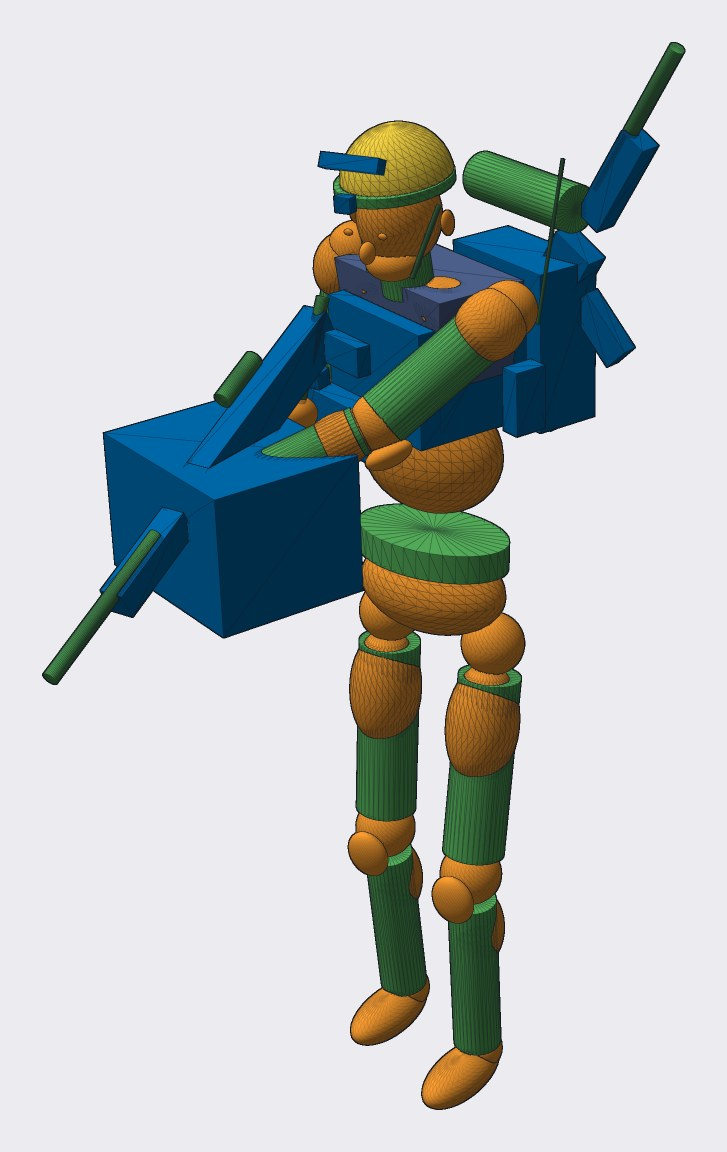
\includegraphics[width=3.53cm]{figures/img/shapes/soldier_prims.jpg}};
\node[anchor=west,inner sep=1pt] (L0) at (3.78,5.04) {Neck};
\draw[black!70,line width=0.4pt] (L0.west) -- (1.99,4.51); \fill[black] (1.99,4.51) circle (0.6pt);
\node[anchor=west,inner sep=1pt] (L1) at (3.78,3.92) {Rifle (slung)};
\draw[black!70,line width=0.4pt] (L1.west) -- (2.78,4.42); \fill[black] (2.78,4.42) circle (0.6pt);
\node[anchor=west,inner sep=1pt] (L2) at (3.78,2.80) {Shoulder};
\draw[black!70,line width=0.4pt] (L2.west) -- (1.51,3.88); \fill[black] (1.51,3.88) circle (0.6pt);
\draw[black!70,line width=0.4pt] (L2.west) -- (1.76,3.64); \fill[black] (1.76,3.64) circle (0.6pt);
\node[anchor=west,inner sep=1pt] (L3) at (3.78,1.68) {Rifle (held)};
\draw[black!70,line width=0.4pt] (L3.west) -- (0.96,3.27); \fill[black] (0.96,3.27) circle (0.6pt);
\node[anchor=west,inner sep=1pt] (L4) at (3.78,0.56) {Hip};
\draw[black!70,line width=0.4pt] (L4.west) -- (2.27,1.32); \fill[black] (2.27,1.32) circle (0.6pt);
\draw[black!70,line width=0.4pt] (L4.west) -- (1.90,1.58); \fill[black] (1.90,1.58) circle (0.6pt);
\end{tikzpicture}\\[-0.3mm]{\fontsize{7.5}{9}\selectfont Full model} & {\fontsize{7.5}{9}\selectfont Made of primitives (pulled apart)}\end{tabular}
\\[0.8mm]{\fontsize{7}{8.5}\selectfont \primchipn{cuboid}{16}\quad \primchipn{taperedbox}{1}\quad \primchipn{sphere}{37}\quad \primchipn{hemisphere}{1}\quad \primchipn{cylinder}{20}\quad \textbf{total 75}\\$^\dagger$ 8 hidden at the start, drawn at rest scale on the right}\vspace{0.6mm}\end{minipage}}
\captionof{figure}{Soldier.}\label{fig:d-soldier}
\end{center}\vspace{-3mm}
\noindent\textbf{Soldier.}\label{des:soldier} On-duty soldier of the camp garrison (friendly, possessable). 8 instances; the first stands 21\,m north of the bunker. Placement of the first: $T(-0.80,\,-0.30,\,21.00)\,R_y(0^\circ)\,S(1)$.
{\fontsize{7}{8.2}\selectfont\setlength{\tabcolsep}{2.6pt}\renewcommand{\arraystretch}{1.02}
\begin{longtable}{@{}>{\raggedright\arraybackslash}p{3.3cm}l>{\raggedright\arraybackslash}p{2.7cm}>{\raggedright\arraybackslash}p{4.2cm}>{\raggedright\arraybackslash}p{2.3cm}>{\raggedright\arraybackslash}p{2.4cm}@{}}
\toprule Part ($\times n$) & Shape & Size $S$ (cm) & Position $T$ (cm, design frame) & Rotation $R$ ($^\circ$) & Parent\\\midrule\endhead
\bottomrule\endfoot
\multicolumn{6}{@{}l}{\textit{Pelvis}}\\[0.2mm]
Hips & \primchip{sphere} & $37.8{\times}22{\times}24$ & $(0,\,101,\,0)$ & -- & Pelvis\\
Belt & \primchip{cylinder} & $38.8{\times}25{\times}7$ & $(0,\,109,\,0)$ & $(90,\,0,\,0)$ & Pelvis\\
\multicolumn{6}{@{}l}{\textit{Hip}}\\[0.2mm]
Hip joint $\times$2 & \primchip{sphere} & $15{\times}15{\times}15$ & $(\pm 10,\,97,\,0)$ & -- & Hip\\
Thigh $\times$2 & \primchip{cylinder} & $15{\times}15{\times}46$ & $(\pm 10,\,\{74,75\},\,\{1,3\})$ & $(90,\,0,\,0)$ & Hip\\
Knee joint $\times$2 & \primchip{sphere} & $15{\times}15{\times}15$ & $(\pm 10,\,\{51,52\},\,\{1,6\})$ & -- & Knee\\
Shin $\times$2 & \primchip{cylinder} & $12{\times}12{\times}44$ & $(\pm 10,\,30,\,\{-2,4\})$ & $(90,\,0,\,0)$ & Knee\\
Ankle joint $\times$2 & \primchip{sphere} & $12{\times}12{\times}12$ & $(\pm 10,\,8,\,\{-6,2\})$ & -- & Ankle\\
Boot $\times$2 & \primchip{sphere} & $13{\times}11{\times}30$ & $(\pm 10,\,6,\,\{0,8\})$ & -- & Ankle\\
Calf $\times$2 & \primchip{sphere} & $13{\times}22{\times}14$ & $(\pm 10,\,39,\,\{-2,3\})$ & -- & Knee\\
Knee pad $\times$2 & \primchip{sphere} & $11.5{\times}13{\times}6$ & $(\pm 10,\,\{48,49\},\,\{7,11\})$ & -- & Knee\\
Thigh muscle $\times$2 & \primchip{sphere} & $17.5{\times}31{\times}18$ & $(\pm 10,\,\{82,83\},\,\{1,3\})$ & -- & Hip\\
\multicolumn{6}{@{}l}{\textit{Spine}}\\[0.2mm]
Abdomen & \primchip{sphere} & $35.7{\times}30{\times}24$ & $(0,\,121,\,0)$ & -- & Spine\\
Torso & \primchip{taperedbox} & $39.9{\times}33{\times}23$ & $(-1,\,141,\,1)$ & $(0,\,0,\,180)$ & Chest\\
Backpack & \primchip{cuboid} & $32{\times}38{\times}16$ & $(6,\,139,\,-18)$ & -- & Chest\\
Bedroll & \primchip{cylinder} & $11{\times}11{\times}34$ & $(6,\,163,\,-18)$ & $(0,\,90,\,0)$ & Chest\\
Rifle receiver $\times$2\,$^\dagger$ & \primchip{cuboid} & $6{\times}11{\times}52$ & $(\{-16,10\},\,\{132,141\},\,\{-29,34\})$ & -- & Rifle (held), Rifle (slung)\\
Rifle barrel $\times$2\,$^\dagger$ & \primchip{cylinder} & $3.5{\times}3.5{\times}40$ & $(\{-16,31\},\,\{112,181\},\,\{-24,75\})$ & -- & Rifle (held), Rifle (slung)\\
Rifle magazine $\times$2\,$^\dagger$ & \primchip{cuboid} & $4{\times}16{\times}7$ & $(\{-16,25\},\,\{117,144\},\,\{-27,38\})$ & $(15,\,0,\,0)$ & Rifle (held), Rifle (slung)\\
Pistol grip $\times$2\,$^\dagger$ & \primchip{cuboid} & $3.5{\times}10{\times}4.5$ & $(\{-16,12\},\,\{125,130\},\,\{-29,19\})$ & $(-20,\,0,\,0)$ & Rifle (held), Rifle (slung)\\
Handguard $\times$2\,$^\dagger$ & \primchip{cuboid} & $5.8{\times}6.8{\times}24$ & $(\{-16,27\},\,\{116,170\},\,\{-25,65\})$ & -- & Rifle (held), Rifle (slung)\\
Optic $\times$2\,$^\dagger$ & \primchip{cylinder} & $4.2{\times}4.2{\times}13$ & $(\{-16,4\},\,\{138,147\},\,\{-30,40\})$ & -- & Rifle (held), Rifle (slung)\\
Carried crate\,$^\dagger$ & \primchip{cuboid} & $46{\times}32{\times}36$ & $(-14,\,120,\,38)$ & -- & Chest\\
Neck & \primchip{cylinder} & $12.5{\times}11.5{\times}11$ & $(-1,\,158,\,3)$ & $(90,\,0,\,0)$ & Neck\\
Head & \primchip{sphere} & $18{\times}22.5{\times}20.5$ & $(-2,\,168,\,5)$ & -- & Head\\
Helmet & \primchip{hemisphere} & $24.5{\times}12.5{\times}26.5$ & $(-3,\,178,\,6)$ & $(-6,\,0,\,0)$ & Head\\
Helmet brim & \primchip{cylinder} & $25.5{\times}28{\times}2.2$ & $(-2,\,174,\,6)$ & $(84,\,0,\,0)$ & Head\\
Jaw & \primchip{sphere} & $13{\times}8.5{\times}11.5$ & $(-2,\,161,\,8)$ & -- & Head\\
Nose & \primchip{sphere} & $3.2{\times}5{\times}4.5$ & $(-2,\,164,\,14)$ & $(-15,\,0,\,0)$ & Head\\
Eye $\times$2 & \primchip{sphere} & $2.4{\times}1.6{\times}1.2$ & $(\{-5,1\},\,\{167,168\},\,15)$ & -- & Head\\
Ear $\times$2 & \primchip{sphere} & $2.2{\times}5.8{\times}4.2$ & $(\{-11,7\},\,\{167,168\},\,5)$ & -- & Head\\
Chin strap $\times$2 & \primchip{cylinder} & $1.2{\times}1.2{\times}17$ & $(\{-8,4\},\,\{164,165\},\,7)$ & $(59,\,\pm 37,\,0)$ & Head\\
Goggles & \primchip{cuboid} & $15{\times}3.2{\times}3$ & $(-3,\,179,\,17)$ & $(-35,\,0,\,0)$ & Head\\
NVG mount & \primchip{cuboid} & $4{\times}3.5{\times}2.5$ & $(-2,\,173,\,20)$ & $(-10,\,0,\,0)$ & Head\\
Trapezius $\times$2 & \primchip{sphere} & $20{\times}8.5{\times}15$ & $(\pm 8,\,153,\,\pm 3)$ & $(0,\,0,\,\pm 20)$ & Neck\\
Shoulder joint $\times$2 & \primchip{sphere} & $13{\times}13{\times}13$ & $(\{-22,20\},\,\{150,151\},\,\{-6,9\})$ & -- & Shoulder\\
Upper arm $\times$2 & \primchip{cylinder} & $13{\times}13{\times}30$ & $(\{-25,13\},\,\{136,141\},\,\{-7,18\})$ & $(90,\,0,\,0)$ & Shoulder\\
Elbow joint $\times$2 & \primchip{sphere} & $13{\times}13{\times}13$ & $(\{-28,5\},\,\{121,132\},\,\{-7,27\})$ & -- & Elbow\\
Forearm $\times$2 & \primchip{cylinder} & $11{\times}11{\times}26$ & $(\{-23,-4\},\,\{125,126\},\,\{4,35\})$ & $(90,\,0,\,0)$ & Elbow\\
Hand $\times$2 & \primchip{sphere} & $9{\times}12{\times}8$ & $(-16,\,\{119,130\},\,\{20,46\})$ & -- & Wrist\\
Forearm muscle $\times$2 & \primchip{sphere} & $12{\times}18{\times}12$ & $(\{-25,1\},\,\{123,129\},\,\{-1,31\})$ & -- & Elbow\\
Elbow pad $\times$2 & \primchip{sphere} & $10{\times}11{\times}5.5$ & $(\{-28,8\},\,\{116,127\},\,\{-5,28\})$ & -- & Elbow\\
Deltoid $\times$2 & \primchip{sphere} & $15.5{\times}17{\times}15$ & $(\{-24,19\},\,\{147,149\},\,\{-6,12\})$ & -- & Shoulder\\
Wrench\,$^\dagger$ & \primchip{cylinder} & $3{\times}3{\times}26$ & $(-15,\,139,\,18)$ & -- & Wrist\\
Plate carrier & \primchip{cuboid} & $34.6{\times}27{\times}29.5$ & $(-1,\,138,\,1)$ & -- & Chest\\
Magazine pouches & \primchip{cuboid} & $25{\times}11{\times}6$ & $(-6,\,131,\,17)$ & -- & Chest\\
Admin pouch & \primchip{cuboid} & $13{\times}7{\times}3.5$ & $(-6,\,142,\,17)$ & -- & Chest\\
Radio & \primchip{cuboid} & $5{\times}15{\times}8$ & $(19,\,136,\,3)$ & -- & Chest\\
Radio antenna & \primchip{cylinder} & $0.8{\times}0.8{\times}36.9$ & $(21,\,162,\,0)$ & $(-81,\,153,\,0)$ & Chest\\
\end{longtable}}
\soldierextras
\FloatBarrier}
\newcommand{\designcardsVehiclesAndAircraft}{%
\needspace{10.6cm}
\begin{center}
\fcolorbox{black!30}{white}{\begin{minipage}{0.975\linewidth}\centering\vspace{0.6mm}
\begin{tabular}{@{}c@{\hspace{3mm}}c@{}}\img{figures/img/shapes/main_battle_tank_model.jpg}{6.23cm} & \begin{tikzpicture}[font=\fontsize{7}{8}\selectfont]
\node[inner sep=0,anchor=south west] at (0,0) {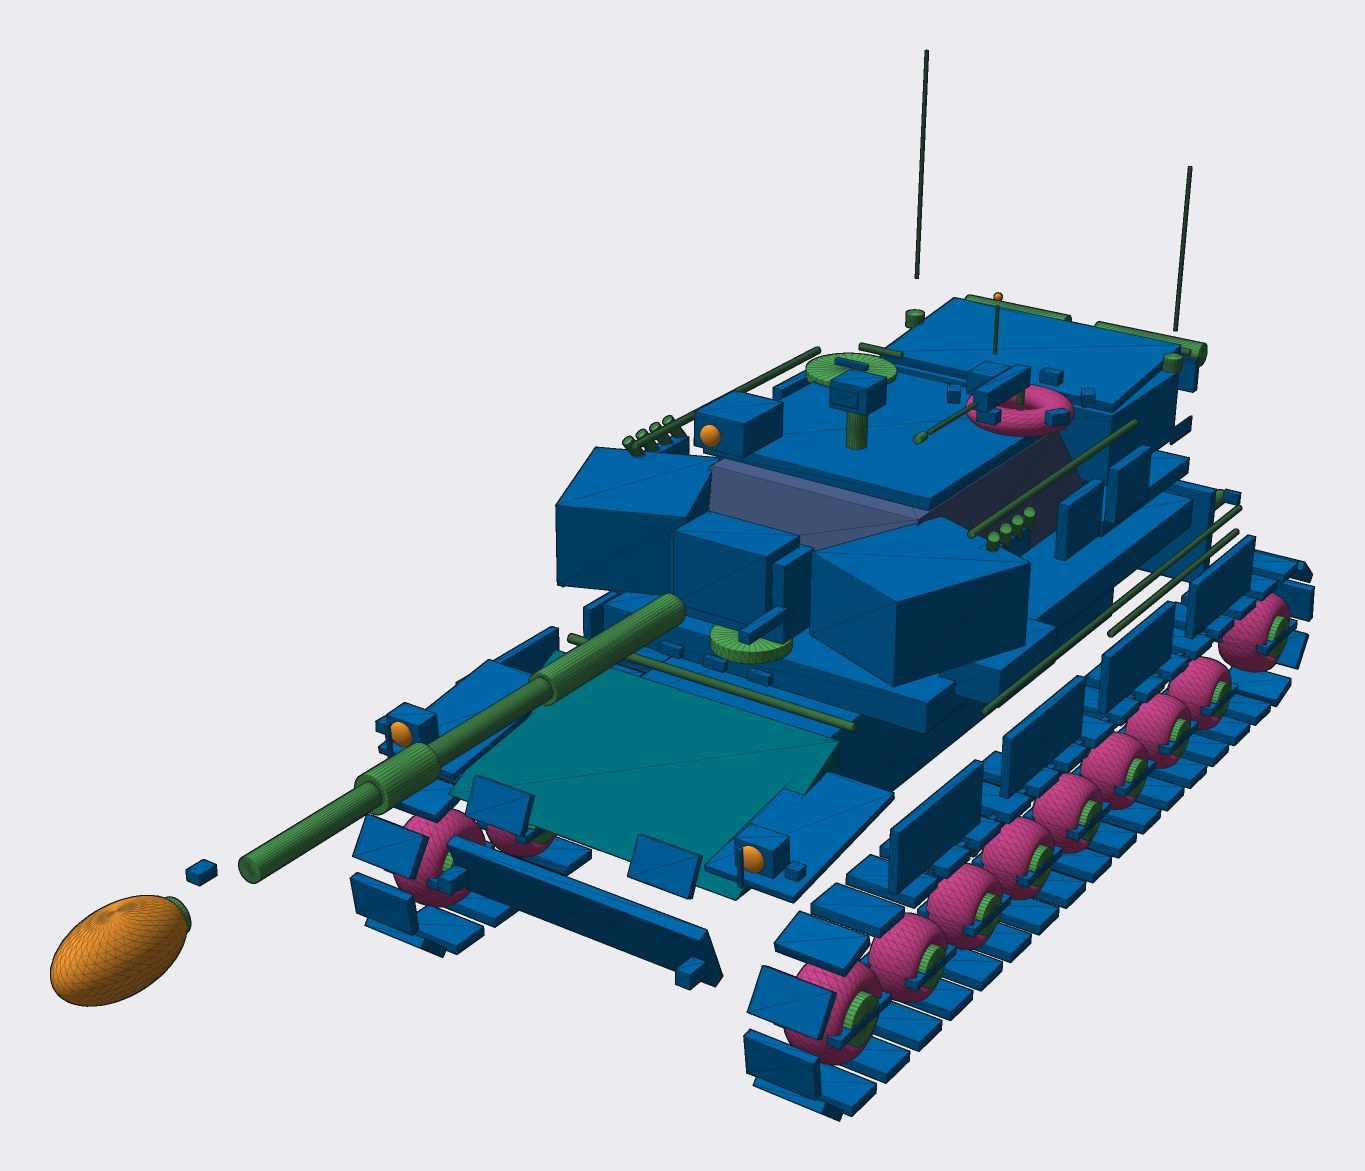
\includegraphics[width=6.53cm]{figures/img/shapes/main_battle_tank_prims.jpg}};
\node[anchor=west,inner sep=1pt] (L0) at (6.78,4.90) {Turret yaw};
\draw[black!70,line width=0.4pt] (L0.west) -- (3.52,3.64); \fill[black] (3.52,3.64) circle (0.6pt);
\node[anchor=west,inner sep=1pt] (L1) at (6.78,3.50) {Drive sprocket};
\draw[black!70,line width=0.4pt] (L1.west) -- (6.00,2.59); \fill[black] (6.00,2.59) circle (0.6pt);
\node[anchor=west,inner sep=1pt] (L2) at (6.78,2.10) {Track};
\draw[black!70,line width=0.4pt] (L2.west) -- (3.38,2.35); \fill[black] (3.38,2.35) circle (0.6pt);
\node[anchor=west,inner sep=1pt] (L3) at (6.78,0.70) {Road wheel};
\draw[black!70,line width=0.4pt] (L3.west) -- (5.73,2.28); \fill[black] (5.73,2.28) circle (0.6pt);
\draw[black!70,line width=0.4pt] (L3.west) -- (5.54,2.10); \fill[black] (5.54,2.10) circle (0.6pt);
\draw[black!70,line width=0.4pt] (L3.west) -- (5.33,1.91); \fill[black] (5.33,1.91) circle (0.6pt);
\draw[black!70,line width=0.4pt] (L3.west) -- (5.10,1.71); \fill[black] (5.10,1.71) circle (0.6pt);
\draw[black!70,line width=0.4pt] (L3.west) -- (4.87,1.50); \fill[black] (4.87,1.50) circle (0.6pt);
\draw[black!70,line width=0.4pt] (L3.west) -- (4.61,1.27); \fill[black] (4.61,1.27) circle (0.6pt);
\draw[black!70,line width=0.4pt] (L3.west) -- (4.34,1.02); \fill[black] (4.34,1.02) circle (0.6pt);
\end{tikzpicture}\\[-0.3mm]{\fontsize{7.5}{9}\selectfont Full model} & {\fontsize{7.5}{9}\selectfont Made of primitives (pulled apart)}\end{tabular}
\\[0.8mm]{\fontsize{7}{8.5}\selectfont \primchipn{cuboid}{168}\quad \primchipn{wedge}{1}\quad \primchipn{taperedbox}{1}\quad \primchipn{sphere}{5}\quad \primchipn{cylinder}{61}\quad \primchipn{torus}{19}\quad \textbf{total 255}\\$^\dagger$ 1 hidden at the start, drawn at rest scale on the right}\vspace{0.6mm}\end{minipage}}
\captionof{figure}{Main battle tank.}\label{fig:d-main_battle_tank}
\end{center}\vspace{-3mm}
\noindent\textbf{Main battle tank.}\label{des:main_battle_tank} User-controllable tracked tank (skid steer, stabilised turret). 3 instances; the first stands 27\,m south-west of the bunker. Placement of the first: $T(-22.00,\,-0.30,\,-16.00)\,R_y(45^\circ)\,S(1)$.
{\fontsize{7}{8.2}\selectfont\setlength{\tabcolsep}{2.6pt}\renewcommand{\arraystretch}{1.02}
\begin{longtable}{@{}>{\raggedright\arraybackslash}p{3.3cm}l>{\raggedright\arraybackslash}p{2.7cm}>{\raggedright\arraybackslash}p{4.2cm}>{\raggedright\arraybackslash}p{2.3cm}>{\raggedright\arraybackslash}p{2.4cm}@{}}
\toprule Part ($\times n$) & Shape & Size $S$ (cm) & Position $T$ (cm, design frame) & Rotation $R$ ($^\circ$) & Parent\\\midrule\endhead
\bottomrule\endfoot
\multicolumn{6}{@{}l}{\textit{Hull}}\\[0.2mm]
Hull core & \primchip{cuboid} & $170{\times}90{\times}560$ & $(0,\,80,\,0)$ & -- & Hull\\
Hull deck & \primchip{cuboid} & $290{\times}26{\times}460$ & $(0,\,129,\,-50)$ & -- & Hull\\
Glacis plate & \primchip{wedge} & $250{\times}64{\times}130$ & $(0,\,116,\,245)$ & -- & Hull\\
Lower nose plate & \primchip{cuboid} & $220{\times}10{\times}52$ & $(0,\,54,\,300)$ & $(67,\,180,\,0)$ & Hull\\
Rear plate & \primchip{cuboid} & $260{\times}90{\times}12$ & $(0,\,85,\,-290)$ & -- & Hull\\
Engine deck & \primchip{cuboid} & $240{\times}14{\times}170$ & $(0,\,147,\,-195)$ & -- & Hull\\
Exhaust grille & \primchip{cuboid} & $150{\times}5{\times}90$ & $(0,\,156,\,-200)$ & -- & Hull\\
Louvre front & \primchip{cuboid} & $150{\times}3{\times}8$ & $(0,\,158,\,-155)$ & -- & Hull\\
Louvre rear & \primchip{cuboid} & $150{\times}3{\times}8$ & $(0,\,158,\,-245)$ & -- & Hull\\
Exhaust pipe $\times$2 & \primchip{cylinder} & $13{\times}13{\times}50$ & $(\pm 90,\,100,\,-310)$ & -- & Hull\\
Front fender $\times$2 & \primchip{cuboid} & $70{\times}5{\times}130$ & $(\pm 110,\,118,\,255)$ & $(8,\,0,\,0)$ & Hull\\
Headlight housing $\times$2 & \primchip{cuboid} & $30{\times}22{\times}20$ & $(\pm 115,\,130,\,300)$ & $(4,\,0,\,0)$ & Hull\\
Headlight lens $\times$2 & \primchip{sphere} & $20{\times}20{\times}10$ & $(\pm 115,\,130,\,310)$ & $(4,\,0,\,0)$ & Hull\\
Tow hook $\times$2 & \primchip{cuboid} & $12{\times}12{\times}20$ & $(\pm 80,\,50,\,312)$ & -- & Hull\\
Spare links $\times$2 & \primchip{cuboid} & $50{\times}30{\times}6$ & $(\pm 55,\,100,\,300)$ & $(-25,\,0,\,0)$ & Hull\\
Stowage box $\times$2 & \primchip{cuboid} & $50{\times}30{\times}90$ & $(\pm 120,\,142,\,60)$ & -- & Hull\\
Fender lamp $\times$2 & \primchip{cuboid} & $10{\times}8{\times}10$ & $(\pm 135,\,125,\,300)$ & -- & Hull\\
Tail light $\times$2 & \primchip{cuboid} & $14{\times}10{\times}6$ & $(\pm 110,\,115,\,-298)$ & -- & Hull\\
Side skirt $\times$8 & \primchip{cuboid} & $7{\times}50{\times}120$ & $(\pm 147,\,95,\,-200{+}125i)$ & -- & Hull\\
Driver hatch & \primchip{cylinder} & $62{\times}62{\times}10$ & $(0,\,150,\,135)$ & $(90,\,0,\,0)$ & Hull\\
Driver periscope $\times$3 & \primchip{cuboid} & $18{\times}8{\times}6$ & $(-30{+}30i,\,150,\,172)$ & -- & Hull\\
Deck edge $\times$2 & \primchip{cylinder} & $5{\times}5{\times}450$ & $(\pm 145,\,142,\,-50)$ & -- & Hull\\
Tow cable $\times$2 & \primchip{cylinder} & $5{\times}5{\times}240$ & $(\pm 149,\,130,\,-120)$ & -- & Hull\\
Skirt rubber flap $\times$2 & \primchip{cuboid} & $5{\times}14{\times}495$ & $(\pm 147,\,64,\,-12)$ & -- & Hull\\
Jerry can $\times$2 & \primchip{cuboid} & $34{\times}46{\times}16$ & $(\pm 45,\,82,\,-305)$ & -- & Hull\\
Headlight guard $\times$2 & \primchip{cuboid} & $3{\times}30{\times}3$ & $(\pm 115,\,130,\,320)$ & $(4,\,0,\,0)$ & Hull\\
Glacis top edge & \primchip{cylinder} & $7{\times}7{\times}250$ & $(0,\,142,\,180)$ & $(0,\,90,\,0)$ & Hull\\
Convoy marker & \primchip{cuboid} & $16{\times}5{\times}2$ & $(0,\,128,\,-297)$ & -- & Hull\\
\multicolumn{6}{@{}l}{\textit{Track}}\\[0.2mm]
Track link $\times$80 & \primchip{cuboid} & $55{\times}8{\times}33$ & $(\pm 110,\,5..105,\,-330..330)$ & $(0..319,\,0,\,0)$ & Track\\
Tyre $\times$18 & \primchip{torus} & $64..76{\times}64..76{\times}133..150$ & $(\pm 110,\,\{44,55\},\,-280..280)$ & -- & Road wheel, Drive sprocket, Idler\\
Hub $\times$18 & \primchip{cylinder} & $32..38{\times}32..38{\times}46..51$ & $(\pm 110,\,\{44,55\},\,-280..280)$ & -- & Road wheel, Drive sprocket, Idler\\
Spoke $\times$18 & \primchip{cuboid} & $57.6..68.4{\times}7{\times}48..53$ & $(\pm 110,\,\{44,55\},\,-280..280)$ & -- & Road wheel, Drive sprocket, Idler\\
Return roller $\times$6 & \primchip{cylinder} & $18{\times}18{\times}20$ & $(\pm 110,\,90,\,-140{+}140i)$ & $(0,\,90,\,0)$ & Track\\
\multicolumn{6}{@{}l}{\textit{Turret yaw}}\\[0.2mm]
Turret body & \primchip{taperedbox} & $230{\times}70{\times}280$ & $(0,\,177,\,-25)$ & -- & Turret yaw\\
Turret cheek $\times$2 & \primchip{cuboid} & $100{\times}66{\times}120$ & $(\pm 95,\,176,\,100)$ & $(0,\,\pm 22,\,0)$ & Turret yaw\\
Turret front plate & \primchip{cuboid} & $100{\times}62{\times}40$ & $(0,\,176,\,135)$ & -- & Turret yaw\\
Turret roof & \primchip{cuboid} & $200{\times}10{\times}220$ & $(0,\,214,\,-25)$ & -- & Turret yaw\\
Bustle & \primchip{cuboid} & $220{\times}62{\times}130$ & $(0,\,176,\,-210)$ & -- & Turret yaw\\
Bustle roof & \primchip{cuboid} & $220{\times}8{\times}130$ & $(0,\,210,\,-210)$ & $(6,\,0,\,0)$ & Turret yaw\\
Stowage basket & \primchip{cuboid} & $230{\times}30{\times}8$ & $(0,\,192,\,-280)$ & -- & Turret yaw\\
Bedroll $\times$2 & \primchip{cylinder} & $20{\times}20{\times}100$ & $(\pm 50,\,204,\,-287)$ & $(0,\,90,\,0)$ & Turret yaw\\
Gunner sight box & \primchip{cuboid} & $45{\times}28{\times}55$ & $(-55,\,232,\,55)$ & -- & Turret yaw\\
Gunner sight lens & \primchip{sphere} & $18{\times}18{\times}12$ & $(-55,\,234,\,85)$ & -- & Turret yaw\\
Cupola ring & \primchip{torus} & $85{\times}85{\times}66.7$ & $(65,\,228,\,-70)$ & $(90,\,0,\,0)$ & Turret yaw\\
Cupola vision block $\times$6 & \primchip{cuboid} & $16{\times}10{\times}10$ & $(30{+}35i,\,237,\,-110..-30)$ & $(0,\,0{+}60i,\,0)$ & Turret yaw\\
Loader hatch & \primchip{cylinder} & $75{\times}75{\times}8$ & $(-65,\,218,\,-90)$ & $(90,\,0,\,0)$ & Turret yaw\\
Loader hatch handle & \primchip{cuboid} & $30{\times}5{\times}5$ & $(-65,\,224,\,-90)$ & -- & Turret yaw\\
MG pintle & \primchip{cylinder} & $6{\times}6{\times}20$ & $(65,\,240,\,-70)$ & $(90,\,0,\,0)$ & MG ring\\
MG receiver & \primchip{cuboid} & $12{\times}16{\times}70$ & $(65,\,250,\,-45)$ & -- & MG elevation\\
MG barrel & \primchip{cylinder} & $4{\times}4{\times}70$ & $(65,\,250,\,15)$ & -- & MG elevation\\
MG flash hider & \primchip{cylinder} & $7{\times}7{\times}10$ & $(65,\,250,\,52)$ & -- & MG elevation\\
MG ammo box & \primchip{cuboid} & $22{\times}18{\times}30$ & $(48,\,247,\,-60)$ & -- & MG elevation\\
Smoke launcher mount $\times$2 & \primchip{cuboid} & $12{\times}20{\times}60$ & $(\pm 118,\,192,\,45)$ & -- & Turret yaw\\
Smoke grenade tube $\times$8 & \primchip{cylinder} & $9{\times}9{\times}22$ & $(\pm 122,\,204,\,25{+}14i)$ & $(-55,\,\pm 30,\,0)$ & Turret yaw\\
Antenna mount $\times$2 & \primchip{cylinder} & $16{\times}16{\times}12$ & $(\pm 90,\,214,\,\{-235,-215\})$ & $(90,\,0,\,0)$ & Turret yaw\\
Whip antenna $\times$2 & \primchip{cylinder} & $3{\times}3{\times}140..200$ & $(\pm 90,\,\{290,320\},\,\{-235,-215\})$ & $(-90,\,0,\,0)$ & Antenna A pivot, Antenna B pivot\\
Gun mantlet & \primchip{cuboid} & $80{\times}58{\times}45$ & $(0,\,184,\,140)$ & -- & Gun pitch\\
Coaxial MG & \primchip{cuboid} & $9{\times}9{\times}50$ & $(38,\,172,\,170)$ & -- & Gun pitch\\
Gun barrel & \primchip{cylinder} & $17{\times}17{\times}420$ & $(0,\,184,\,375)$ & -- & Barrel recoil\\
Thermal sleeve & \primchip{cylinder} & $24{\times}24{\times}150$ & $(0,\,184,\,265)$ & -- & Barrel recoil\\
Fume extractor & \primchip{cylinder} & $27{\times}27{\times}50$ & $(0,\,184,\,435)$ & -- & Barrel recoil\\
Muzzle brake & \primchip{cylinder} & $23{\times}23{\times}34$ & $(0,\,184,\,595)$ & -- & Barrel recoil\\
Muzzle flash\,$^\dagger$ & \primchip{sphere} & $50{\times}50{\times}90$ & $(0,\,184,\,615)$ & -- & Barrel recoil\\
Muzzle bore & \primchip{cylinder} & $12{\times}12{\times}2$ & $(0,\,184,\,612)$ & -- & Barrel recoil\\
Muzzle reference sensor & \primchip{cuboid} & $10{\times}7{\times}14$ & $(0,\,197,\,565)$ & -- & Barrel recoil\\
Side armour block $\times$4 & \primchip{cuboid} & $9{\times}46{\times}60$ & $(\pm 120,\,178,\,\{-113,-47\})$ & -- & Turret yaw\\
Turret roof edge $\times$2 & \primchip{cylinder} & $6{\times}6{\times}270$ & $(\pm 114,\,212,\,-25)$ & -- & Turret yaw\\
Turret number $\times$2 & \primchip{cuboid} & $1.2{\times}13{\times}38$ & $(\pm 111,\,180,\,-210)$ & -- & Turret yaw\\
Bustle rear edge & \primchip{cylinder} & $6{\times}6{\times}220$ & $(0,\,208,\,-275)$ & $(0,\,90,\,0)$ & Turret yaw\\
Panoramic sight post & \primchip{cylinder} & $16{\times}16{\times}30$ & $(5,\,232,\,20)$ & $(90,\,0,\,0)$ & Turret yaw\\
Panoramic sight head & \primchip{cuboid} & $32{\times}22{\times}30$ & $(5,\,254,\,20)$ & -- & Turret yaw\\
Panoramic sight window & \primchip{cuboid} & $24{\times}12{\times}2$ & $(5,\,255,\,36)$ & -- & Turret yaw\\
Wind sensor mast & \primchip{cylinder} & $3{\times}3{\times}42$ & $(0,\,240,\,-160)$ & $(90,\,0,\,0)$ & Turret yaw\\
Wind sensor head & \primchip{sphere} & $7{\times}7{\times}7$ & $(0,\,262,\,-160)$ & -- & Turret yaw\\
Loader hatch hinge & \primchip{cylinder} & $6{\times}6{\times}40$ & $(-65,\,222,\,-127)$ & $(0,\,90,\,0)$ & Turret yaw\\
\end{longtable}}
\tankextras

\needspace{10.6cm}
\begin{center}
\fcolorbox{black!30}{white}{\begin{minipage}{0.975\linewidth}\centering\vspace{0.6mm}
\begin{tabular}{@{}c@{\hspace{3mm}}c@{}}\img{figures/img/shapes/mlrs_rocket_truck_model.jpg}{7.04cm} & \begin{tikzpicture}[font=\fontsize{7}{8}\selectfont]
\node[inner sep=0,anchor=south west] at (0,0) {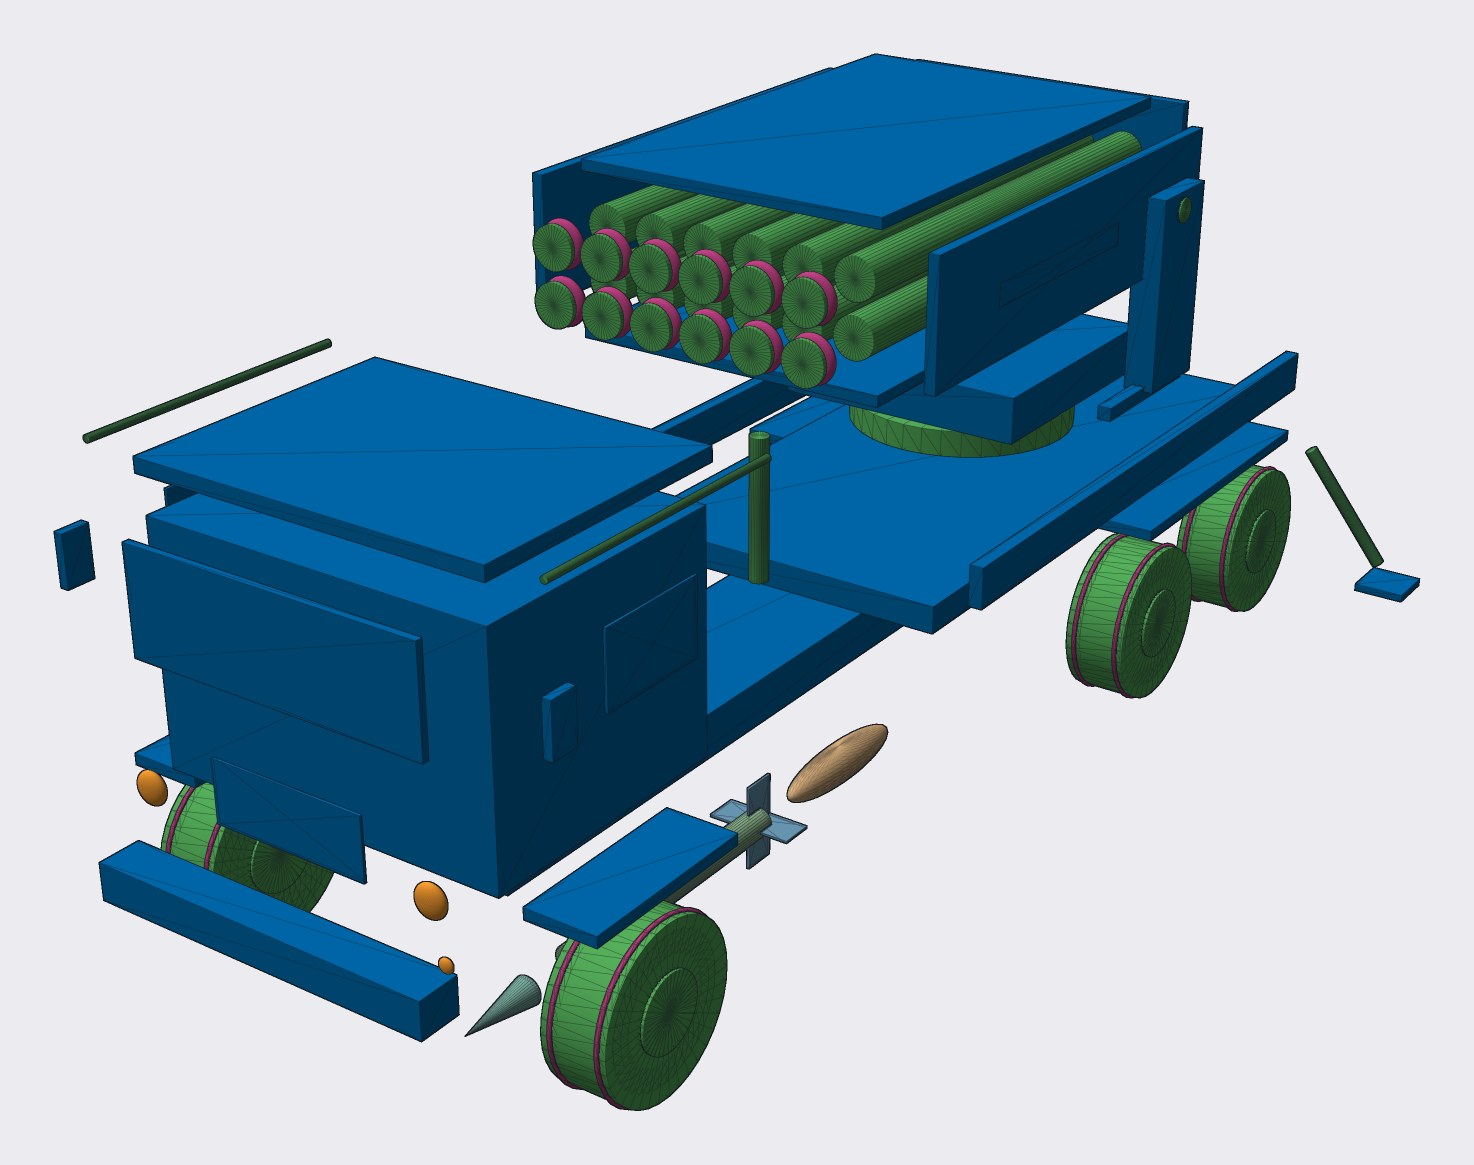
\includegraphics[width=7.09cm]{figures/img/shapes/mlrs_rocket_truck_prims.jpg}};
\node[anchor=west,inner sep=1pt] (L0) at (7.34,4.67) {Mount};
\draw[black!70,line width=0.4pt] (L0.west) -- (4.21,4.15); \fill[black] (4.21,4.15) circle (0.6pt);
\node[anchor=west,inner sep=1pt] (L1) at (7.34,2.80) {Truck};
\draw[black!70,line width=0.4pt] (L1.west) -- (4.21,3.08); \fill[black] (4.21,3.08) circle (0.6pt);
\node[anchor=west,inner sep=1pt] (L2) at (7.34,0.93) {Rocket};
\draw[black!70,line width=0.4pt] (L2.west) -- (3.39,1.45); \fill[black] (3.39,1.45) circle (0.6pt);
\draw[black!70,line width=0.4pt] (L2.west) -- (3.39,1.45); \fill[black] (3.39,1.45) circle (0.6pt);
\draw[black!70,line width=0.4pt] (L2.west) -- (3.39,1.45); \fill[black] (3.39,1.45) circle (0.6pt);
\draw[black!70,line width=0.4pt] (L2.west) -- (3.39,1.45); \fill[black] (3.39,1.45) circle (0.6pt);
\draw[black!70,line width=0.4pt] (L2.west) -- (3.39,1.45); \fill[black] (3.39,1.45) circle (0.6pt);
\draw[black!70,line width=0.4pt] (L2.west) -- (3.39,1.45); \fill[black] (3.39,1.45) circle (0.6pt);
\end{tikzpicture}\\[-0.3mm]{\fontsize{7.5}{9}\selectfont Full model} & {\fontsize{7.5}{9}\selectfont Made of primitives (pulled apart)}\end{tabular}
\\[0.8mm]{\fontsize{7}{8.5}\selectfont \primchipn{cube}{1}\quad \primchipn{cuboid}{32}\quad \primchipn{sphere}{3}\quad \primchipn{cylinder}{46}\quad \primchipn{torus}{24}\quad \textbf{total 106}\\pale: MLRS rocket $\times$6 (30 parts)}\vspace{0.6mm}\end{minipage}}
\captionof{figure}{MLRS rocket truck.}\label{fig:d-mlrs_rocket_truck}
\end{center}\vspace{-3mm}
\noindent\textbf{MLRS rocket truck.}\label{des:mlrs_rocket_truck} 6x2 rocket truck with a rotating, elevating 12-tube pod (user controlled). One instance, 25\,m north-west of the bunker. Placement of the first: $T(-11.50,\,-0.30,\,22.50)\,R_y(-15^\circ)\,S(1)$.
{\fontsize{7}{8.2}\selectfont\setlength{\tabcolsep}{2.6pt}\renewcommand{\arraystretch}{1.02}
\begin{longtable}{@{}>{\raggedright\arraybackslash}p{3.3cm}l>{\raggedright\arraybackslash}p{2.7cm}>{\raggedright\arraybackslash}p{4.2cm}>{\raggedright\arraybackslash}p{2.3cm}>{\raggedright\arraybackslash}p{2.4cm}@{}}
\toprule Part ($\times n$) & Shape & Size $S$ (cm) & Position $T$ (cm, design frame) & Rotation $R$ ($^\circ$) & Parent\\\midrule\endhead
\bottomrule\endfoot
\multicolumn{6}{@{}l}{\textit{Truck}}\\[0.2mm]
Chassis & \primchip{cuboid} & $110{\times}32{\times}800$ & $(0,\,95,\,0)$ & -- & Truck\\
Cab & \primchip{cuboid} & $245{\times}160{\times}190$ & $(0,\,195,\,300)$ & -- & Truck\\
Cab roof armour & \primchip{cuboid} & $250{\times}10{\times}195$ & $(0,\,280,\,300)$ & -- & Truck\\
Windscreen & \primchip{cuboid} & $210{\times}70{\times}5$ & $(0,\,230,\,397)$ & -- & Truck\\
Bumper & \primchip{cuboid} & $240{\times}25{\times}30$ & $(0,\,100,\,410)$ & -- & Truck\\
Headlight $\times$2 & \primchip{sphere} & $22{\times}22{\times}10$ & $(\pm 80,\,140,\,398)$ & -- & Truck\\
Mirror $\times$2 & \primchip{cuboid} & $6{\times}35{\times}20$ & $(\pm 135,\,230,\,380)$ & -- & Truck\\
Cab tactical lamp & \primchip{sphere} & $10{\times}10{\times}5$ & $(90,\,115,\,402)$ & -- & Truck\\
Bed deck & \primchip{cuboid} & $250{\times}20{\times}500$ & $(0,\,125,\,-160)$ & -- & Truck\\
Bed side $\times$2 & \primchip{cuboid} & $10{\times}30{\times}500$ & $(\pm 120,\,150,\,-160)$ & -- & Truck\\
Wheel $\times$6 & \primchip{cylinder} & $115{\times}115{\times}45$ & $(\pm 115,\,57,\,\{-300,-160,310\})$ & $(0,\,90,\,0)$ & Truck\\
Wheel hub $\times$6 & \primchip{cylinder} & $51.7{\times}51.7{\times}49$ & $(\pm 115,\,57,\,\{-300,-160,310\})$ & $(0,\,90,\,0)$ & Truck\\
Fender $\times$4 & \primchip{cuboid} & $50{\times}8{\times}130..240$ & $(\pm 115,\,120,\,\{-230,310\})$ & -- & Truck\\
Outrigger $\times$2 & \primchip{cylinder} & $10{\times}10{\times}113$ & $(\pm 150,\,53,\,-390)$ & $(56,\,\pm 108,\,0)$ & Truck\\
Outrigger pad $\times$2 & \primchip{cuboid} & $40{\times}6{\times}40$ & $(\pm 180,\,3,\,-400)$ & -- & Truck\\
Cab side window $\times$2 & \primchip{cuboid} & $2{\times}50{\times}80$ & $(\pm 123,\,230,\,305)$ & -- & Truck\\
Cab roof edge $\times$2 & \primchip{cylinder} & $5{\times}5{\times}194$ & $(\pm 125,\,285,\,300)$ & -- & Truck\\
Radiator grille & \primchip{cuboid} & $110{\times}42{\times}2$ & $(0,\,150,\,396)$ & -- & Truck\\
Exhaust stack & \primchip{cylinder} & $12{\times}12{\times}90$ & $(100,\,245,\,195)$ & $(90,\,0,\,0)$ & Truck\\
Tyre tread $\times$12 & \primchip{torus} & $118{\times}118{\times}30$ & $(\pm(102{+}26i),\,57,\,\{-300,-160,310\})$ & $(0,\,90,\,0)$ & Truck\\
\multicolumn{6}{@{}l}{\textit{Mount}}\\[0.2mm]
Slew ring & \primchip{cylinder} & $170{\times}170{\times}20$ & $(0,\,145,\,-160)$ & $(90,\,0,\,0)$ & Mount\\
Mount base & \primchip{cuboid} & $190{\times}35{\times}190$ & $(0,\,173,\,-160)$ & -- & Mount\\
Pod arm $\times$2 & \primchip{cuboid} & $22{\times}140{\times}60$ & $(\pm 122,\,240,\,-160)$ & -- & Mount\\
Arm brace $\times$2 & \primchip{cuboid} & $10{\times}10{\times}110$ & $(\pm 122,\,185,\,-140)$ & -- & Mount\\
Ram foot & \primchip{cuboid} & $30{\times}12{\times}30$ & $(0,\,187,\,-250)$ & -- & Mount\\
Ram cylinder & \primchip{cylinder} & $16{\times}16{\times}31.6$ & $(0,\,204,\,-242)$ & $(-59,\,0,\,0)$ & Mount\\
Ram rod & \primchip{cylinder} & $9{\times}9{\times}28.7$ & $(0,\,228,\,-227)$ & $(-59,\,0,\,0)$ & Mount\\
Pod side plate $\times$2 & \primchip{cuboid} & $8{\times}90{\times}360$ & $(\pm 117,\,285,\,-60)$ & -- & Pod\\
Trunnion $\times$2 & \primchip{cylinder} & $18{\times}18{\times}30$ & $(\pm 120,\,285,\,-160)$ & $(0,\,90,\,0)$ & Pod\\
Pod frame $\times$2 & \primchip{cuboid} & $230{\times}8{\times}360$ & $(0,\,\{241,329\},\,-60)$ & -- & Pod\\
Pod rear plate & \primchip{cuboid} & $230{\times}90{\times}8$ & $(0,\,285,\,-244)$ & -- & Pod\\
Ram lug & \primchip{cube} & $20{\times}20{\times}20$ & $(0,\,240,\,-220)$ & -- & Pod\\
Launch tube $\times$12 & \primchip{cylinder} & $30{\times}30{\times}360$ & $(\pm(17{+}34i),\,\{268,302\},\,-60)$ & -- & Tube\\
Muzzle ring $\times$12 & \primchip{torus} & $34{\times}34{\times}26.7$ & $(\pm(17{+}34i),\,\{268,302\},\,114)$ & -- & Tube\\
Tube cap $\times$12 & \primchip{cylinder} & $31{\times}31{\times}4$ & $(\pm(17{+}34i),\,\{268,302\},\,121)$ & -- & Tube\\
Pod stencil $\times$2 & \primchip{cuboid} & $0.6{\times}16{\times}160$ & $(\pm 121,\,285,\,-40)$ & -- & Pod\\
\multicolumn{6}{@{}l}{\textit{MLRS rocket truck}}\\[0.2mm]
\textit{MLRS rocket} $\times$6 & \multicolumn{5}{@{}l}{\textit{nested design, drawn pale; its parts are counted in its own card (Figure~\ref{fig:d-mlrs_rocket})}}\\
\end{longtable}}

\needspace{10.6cm}
\begin{center}
\fcolorbox{black!30}{white}{\begin{minipage}{0.975\linewidth}\centering\vspace{0.6mm}
\begin{tabular}{@{}c@{\hspace{3mm}}c@{}}\img{figures/img/shapes/scout_helicopter_model.jpg}{7.30cm} & \begin{tikzpicture}[font=\fontsize{7}{8}\selectfont]
\node[inner sep=0,anchor=south west] at (0,0) {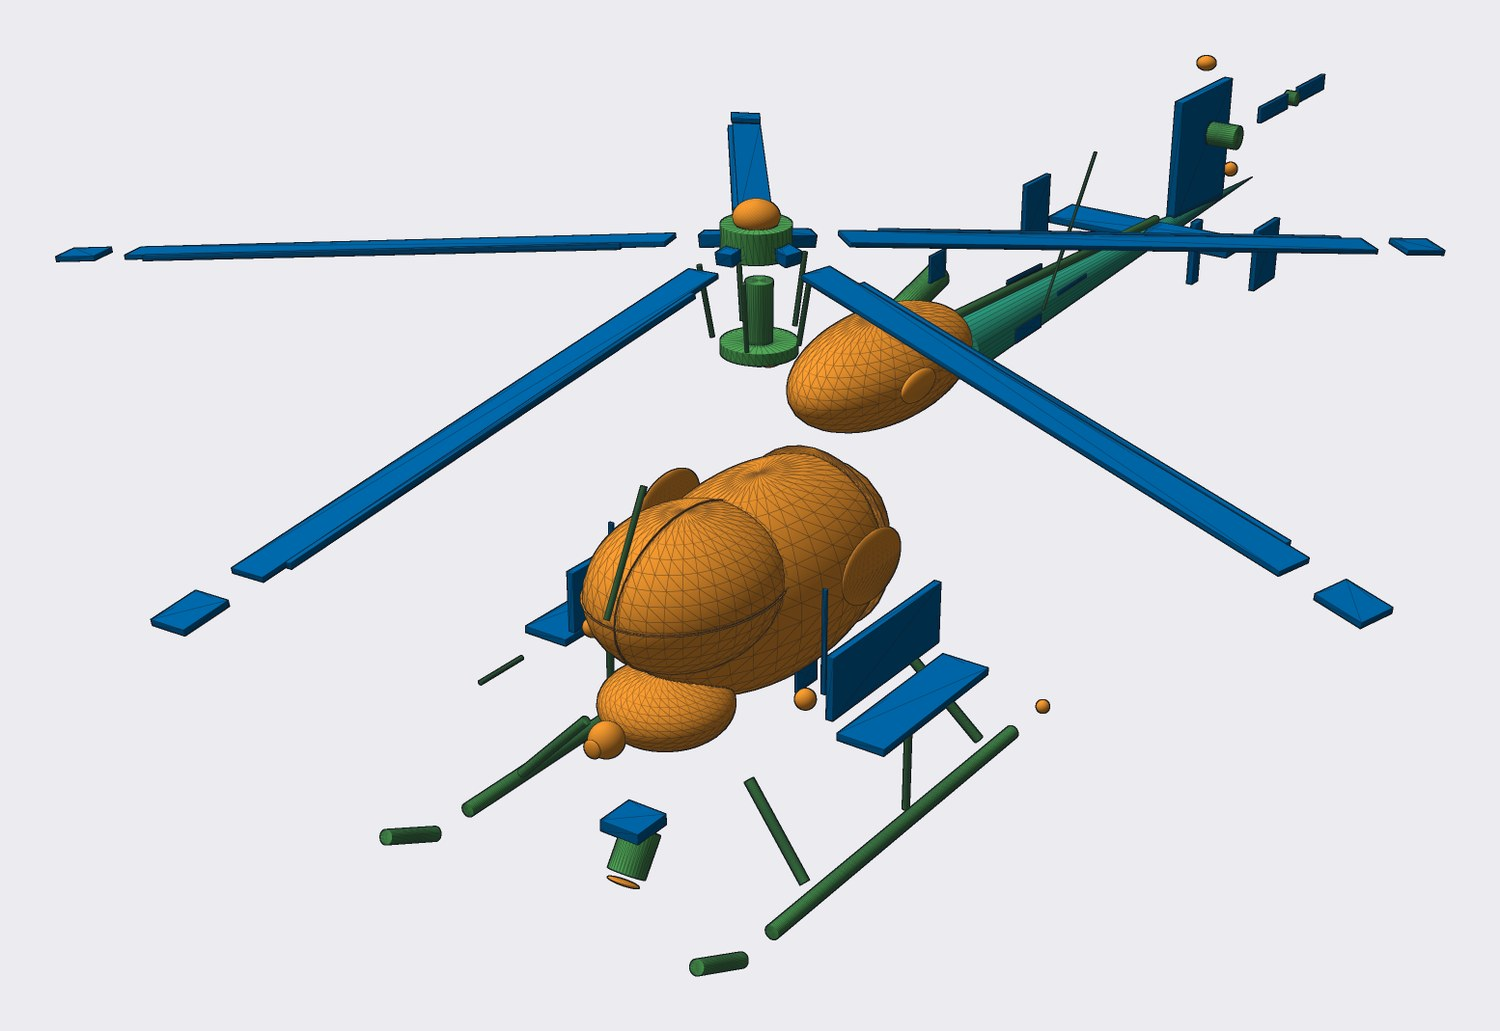
\includegraphics[width=6.90cm]{figures/img/shapes/scout_helicopter_prims.jpg}};
\node[anchor=west,inner sep=1pt] (L0) at (7.15,4.40) {Tail rotor mount};
\draw[black!70,line width=0.4pt] (L0.west) -- (5.94,4.29); \fill[black] (5.94,4.29) circle (0.6pt);
\node[anchor=west,inner sep=1pt] (L1) at (7.15,3.73) {Blade 4 pivot};
\draw[black!70,line width=0.4pt] (L1.west) -- (3.46,3.98); \fill[black] (3.46,3.98) circle (0.6pt);
\node[anchor=west,inner sep=1pt] (L2) at (7.15,3.05) {Blade 3 pivot};
\draw[black!70,line width=0.4pt] (L2.west) -- (5.14,3.64); \fill[black] (5.14,3.64) circle (0.6pt);
\node[anchor=west,inner sep=1pt] (L3) at (7.15,2.37) {Blade 5 pivot};
\draw[black!70,line width=0.4pt] (L3.west) -- (1.80,3.62); \fill[black] (1.80,3.62) circle (0.6pt);
\node[anchor=west,inner sep=1pt] (L4) at (7.15,1.69) {Blade 2 pivot};
\draw[black!70,line width=0.4pt] (L4.west) -- (4.75,2.89); \fill[black] (4.75,2.89) circle (0.6pt);
\node[anchor=west,inner sep=1pt] (L5) at (7.15,1.02) {Blade 1 pivot};
\draw[black!70,line width=0.4pt] (L5.west) -- (2.29,2.87); \fill[black] (2.29,2.87) circle (0.6pt);
\node[anchor=west,inner sep=1pt] (L6) at (7.15,0.34) {Searchlight pan};
\draw[black!70,line width=0.4pt] (L6.west) -- (2.92,0.83); \fill[black] (2.92,0.83) circle (0.6pt);
\end{tikzpicture}\\[-0.3mm]{\fontsize{7.5}{9}\selectfont Full model} & {\fontsize{7.5}{9}\selectfont Made of primitives (pulled apart)}\end{tabular}
\\[0.8mm]{\fontsize{7}{8.5}\selectfont \primchipn{cuboid}{40}\quad \primchipn{sphere}{21}\quad \primchipn{cylinder}{28}\quad \primchipn{frustum}{1}\quad \primchipn{cone}{1}\quad \textbf{total 91}}\vspace{0.6mm}\end{minipage}}
\captionof{figure}{Scout helicopter.}\label{fig:d-scout_helicopter}
\end{center}\vspace{-3mm}
\noindent\textbf{Scout helicopter.}\label{des:scout_helicopter} MH-6 style light helicopter (user-controllable). One instance, 26\,m north-east of the bunker. Placement of the first: $T(20.30,\,-0.18,\,17.00)\,R_y(-130^\circ)\,S(1)$.
{\fontsize{7}{8.2}\selectfont\setlength{\tabcolsep}{2.6pt}\renewcommand{\arraystretch}{1.02}
\begin{longtable}{@{}>{\raggedright\arraybackslash}p{3.3cm}l>{\raggedright\arraybackslash}p{2.7cm}>{\raggedright\arraybackslash}p{4.2cm}>{\raggedright\arraybackslash}p{2.3cm}>{\raggedright\arraybackslash}p{2.4cm}@{}}
\toprule Part ($\times n$) & Shape & Size $S$ (cm) & Position $T$ (cm, design frame) & Rotation $R$ ($^\circ$) & Parent\\\midrule\endhead
\bottomrule\endfoot
\multicolumn{6}{@{}l}{\textit{Body}}\\[0.2mm]
Cabin & \primchip{sphere} & $135{\times}145{\times}250$ & $(0,\,118,\,0)$ & -- & Body\\
Canopy glass & \primchip{sphere} & $122{\times}105{\times}150$ & $(0,\,136,\,62)$ & -- & Body\\
Chin nose & \primchip{sphere} & $90{\times}50{\times}90$ & $(0,\,78,\,80)$ & -- & Body\\
Door seam left & \primchip{cuboid} & $3{\times}75{\times}2$ & $(66,\,114,\,38)$ & -- & Body\\
Door seam right & \primchip{cuboid} & $3{\times}75{\times}2$ & $(-66,\,114,\,38)$ & -- & Body\\
Engine cowling & \primchip{sphere} & $95{\times}75{\times}190$ & $(0,\,195,\,-115)$ & -- & Body\\
Engine exhaust & \primchip{cylinder} & $20{\times}20{\times}55$ & $(-35,\,200,\,-210)$ & $(15,\,0,\,0)$ & Body\\
Rotor mast & \primchip{cylinder} & $18{\times}18{\times}55$ & $(0,\,255,\,0)$ & $(90,\,0,\,0)$ & Body\\
Tail boom & \primchip{cone} & $45{\times}45{\times}520$ & $(0,\,180,\,-390)$ & $(0,\,180,\,0)$ & Body\\
Tail fin & \primchip{cuboid} & $7{\times}105{\times}95$ & $(0,\,220,\,-500)$ & -- & Body\\
Horizontal stabiliser & \primchip{cuboid} & $160{\times}5{\times}40$ & $(0,\,185,\,-430)$ & -- & Body\\
Stabiliser plate left & \primchip{cuboid} & $4{\times}50{\times}40$ & $(80,\,185,\,-430)$ & -- & Body\\
Stabiliser plate right & \primchip{cuboid} & $4{\times}50{\times}40$ & $(-80,\,185,\,-430)$ & -- & Body\\
Tail bumper & \primchip{cuboid} & $5{\times}55{\times}12$ & $(0,\,150,\,-505)$ & -- & Body\\
Skid right & \primchip{cylinder} & $10{\times}10{\times}300$ & $(-95,\,5,\,10)$ & -- & Body\\
Skid toe right & \primchip{cylinder} & $10{\times}10{\times}50$ & $(-95,\,12,\,168)$ & $(-25,\,0,\,0)$ & Body\\
Front strut right & \primchip{cylinder} & $7{\times}7{\times}73.5$ & $(-70,\,31,\,85)$ & $(-46,\,101,\,0)$ & Body\\
Rear strut right & \primchip{cylinder} & $7{\times}7{\times}73.5$ & $(-70,\,31,\,-75)$ & $(-46,\,79,\,0)$ & Body\\
Skid left & \primchip{cylinder} & $10{\times}10{\times}300$ & $(95,\,5,\,10)$ & -- & Body\\
Skid toe left & \primchip{cylinder} & $10{\times}10{\times}50$ & $(95,\,12,\,168)$ & $(-25,\,0,\,0)$ & Body\\
Front strut left & \primchip{cylinder} & $7{\times}7{\times}73.5$ & $(70,\,31,\,85)$ & $(-46,\,-101,\,0)$ & Body\\
Rear strut left & \primchip{cylinder} & $7{\times}7{\times}73.5$ & $(70,\,31,\,-75)$ & $(-46,\,-79,\,0)$ & Body\\
Nav light left (red) & \primchip{sphere} & $14{\times}14{\times}14$ & $(66,\,90,\,55)$ & -- & Body\\
Nav light right (green) & \primchip{sphere} & $14{\times}14{\times}14$ & $(-66,\,90,\,55)$ & -- & Body\\
Nav light tail (white) & \primchip{sphere} & $12{\times}12{\times}12$ & $(0,\,195,\,-552)$ & -- & Body\\
Anti-collision strobe & \primchip{sphere} & $16{\times}12{\times}16$ & $(0,\,278,\,-500)$ & -- & Body\\
Swashplate & \primchip{cylinder} & $50{\times}50{\times}8$ & $(0,\,242,\,0)$ & $(90,\,0,\,0)$ & Body\\
Pitch link $\times$5 & \primchip{cylinder} & $3{\times}3{\times}48.7$ & $(-22..26,\,266,\,-25..24)$ & $(-81,\,-124{+}72i,\,0)$ & Body\\
Bench seat right & \primchip{cuboid} & $35{\times}5{\times}130$ & $(-98,\,75,\,5)$ & -- & Body\\
Bench back right & \primchip{cuboid} & $5{\times}45{\times}130$ & $(-80,\,100,\,5)$ & -- & Body\\
Bench strut right & \primchip{cylinder} & $5{\times}5{\times}67$ & $(-95,\,38,\,5)$ & $(-90,\,0,\,0)$ & Body\\
Bench seat left & \primchip{cuboid} & $35{\times}5{\times}130$ & $(98,\,75,\,5)$ & -- & Body\\
Bench back left & \primchip{cuboid} & $5{\times}45{\times}130$ & $(80,\,100,\,5)$ & -- & Body\\
Bench strut left & \primchip{cylinder} & $5{\times}5{\times}67$ & $(95,\,38,\,5)$ & $(-90,\,0,\,0)$ & Body\\
Wire cutter & \primchip{cylinder} & $4{\times}4{\times}85$ & $(0,\,173,\,110)$ & $(-62,\,180,\,0)$ & Body\\
Whip antenna & \primchip{cylinder} & $2{\times}2{\times}121$ & $(30,\,235,\,-265)$ & $(-65,\,169,\,0)$ & Body\\
Tail rotor gearbox & \primchip{cylinder} & $20{\times}20{\times}30$ & $(10,\,230,\,-510)$ & $(0,\,90,\,0)$ & Body\\
Pitot tube & \primchip{cylinder} & $3{\times}3{\times}40$ & $(-50,\,110,\,145)$ & -- & Body\\
Canopy centre frame & \primchip{sphere} & $4{\times}107{\times}152$ & $(0,\,136,\,62)$ & -- & Body\\
Canopy sill frame & \primchip{sphere} & $125{\times}4{\times}152$ & $(0,\,136,\,62)$ & -- & Body\\
Cabin panel seam & \primchip{sphere} & $125{\times}135{\times}3$ & $(0,\,118,\,-50)$ & -- & Body\\
Door window right & \primchip{sphere} & $10{\times}50{\times}70$ & $(-63,\,136,\,-8)$ & -- & Body\\
Engine intake right & \primchip{sphere} & $10{\times}22{\times}42$ & $(-44,\,205,\,-80)$ & -- & Body\\
Tail number right & \primchip{cuboid} & $1{\times}11{\times}42$ & $(-18,\,180,\,-245)$ & $(0,\,-2,\,0)$ & Body\\
Formation light right & \primchip{cuboid} & $1.2{\times}3{\times}50$ & $(-16,\,190,\,-300)$ & $(0,\,-2,\,0)$ & Body\\
Skid end cap right & \primchip{sphere} & $10{\times}10{\times}10$ & $(-95,\,5,\,-140)$ & -- & Body\\
Door window left & \primchip{sphere} & $10{\times}50{\times}70$ & $(63,\,136,\,-8)$ & -- & Body\\
Engine intake left & \primchip{sphere} & $10{\times}22{\times}42$ & $(44,\,205,\,-80)$ & -- & Body\\
Tail number left & \primchip{cuboid} & $1{\times}11{\times}42$ & $(18,\,180,\,-245)$ & $(0,\,2,\,0)$ & Body\\
Formation light left & \primchip{cuboid} & $1.2{\times}3{\times}50$ & $(16,\,190,\,-300)$ & $(0,\,2,\,0)$ & Body\\
Skid end cap left & \primchip{sphere} & $10{\times}10{\times}10$ & $(95,\,5,\,-140)$ & -- & Body\\
FLIR ball & \primchip{sphere} & $24{\times}24{\times}24$ & $(0,\,80,\,128)$ & -- & Body\\
FLIR window & \primchip{sphere} & $13{\times}13{\times}5$ & $(0,\,80,\,139)$ & -- & Body\\
Drive shaft cover & \primchip{cylinder} & $7{\times}7{\times}330$ & $(0,\,194,\,-315)$ & $(2,\,180,\,0)$ & Body\\
Belly antenna & \primchip{cuboid} & $2{\times}18{\times}25$ & $(0,\,38,\,-45)$ & -- & Body\\
VHF antenna & \primchip{cuboid} & $2{\times}20{\times}20$ & $(0,\,235,\,-170)$ & -- & Body\\
\multicolumn{6}{@{}l}{\textit{Rotor head}}\\[0.2mm]
Rotor hub & \primchip{cylinder} & $45{\times}45{\times}20$ & $(0,\,282,\,0)$ & $(90,\,0,\,0)$ & Main rotor\\
Rotor hub cap & \primchip{sphere} & $30{\times}22{\times}30$ & $(0,\,293,\,0)$ & -- & Main rotor\\
Blade $\times$5 & \primchip{cuboid} & $22{\times}3{\times}390$ & $(-213..213,\,256,\,\{-181,69,224\})$ & -- & Blade 1 flap, Blade 2 flap, Blade 3 flap, Blade 4 flap, Blade 5 flap\\
Blade grip $\times$5 & \primchip{cuboid} & $12{\times}8{\times}35$ & $(-43..43,\,278,\,\{-36,14,45\})$ & -- & Blade 1 flap, Blade 2 flap, Blade 3 flap, Blade 4 flap, Blade 5 flap\\
Blade tip cap $\times$5 & \primchip{cuboid} & $23{\times}3.5{\times}30$ & $(-383..383,\,234,\,\{-325,124,402\})$ & -- & Blade 1 flap, Blade 2 flap, Blade 3 flap, Blade 4 flap, Blade 5 flap\\
Blade erosion strip $\times$5 & \primchip{cuboid} & $3.5{\times}3.6{\times}345$ & $(-214..220,\,256,\,-191..229)$ & -- & Blade 1 flap, Blade 2 flap, Blade 3 flap, Blade 4 flap, Blade 5 flap\\
Main rotor blur disc & \primchip{cylinder} & $840{\times}840{\times}2$ & $(0,\,292,\,0)$ & $(90,\,0,\,0)$ & Tip-path plane\\
\multicolumn{6}{@{}l}{\textit{Tail rotor mount}}\\[0.2mm]
Tail rotor hub & \primchip{cylinder} & $12{\times}12{\times}10$ & $(20,\,230,\,-510)$ & $(0,\,90,\,0)$ & Tail rotor\\
Tail blade $\times$2 & \primchip{cuboid} & $3{\times}13{\times}55$ & $(20,\,230,\,\{-540,-480\})$ & -- & Tail rotor\\
Tail rotor blur disc & \primchip{cylinder} & $120{\times}120{\times}1$ & $(23,\,230,\,-510)$ & $(0,\,90,\,0)$ & Tail rotor mount\\
\multicolumn{6}{@{}l}{\textit{Searchlight pan}}\\[0.2mm]
Searchlight yoke & \primchip{cuboid} & $30{\times}8{\times}30$ & $(0,\,47,\,90)$ & -- & Searchlight pan\\
Searchlight housing & \primchip{cylinder} & $26{\times}26{\times}30$ & $(0,\,30,\,90)$ & -- & Searchlight tilt\\
Searchlight lens & \primchip{sphere} & $22{\times}22{\times}4$ & $(0,\,17,\,99)$ & -- & Searchlight tilt\\
Searchlight cone & \primchip{frustum} & $100{\times}100{\times}100$ & $(0,\,14,\,101)$ & -- & Searchlight tilt\\
\end{longtable}}
\heliextras

\needspace{10.6cm}
\begin{center}
\fcolorbox{black!30}{white}{\begin{minipage}{0.975\linewidth}\centering\vspace{0.6mm}
\begin{tabular}{@{}c@{\hspace{3mm}}c@{}}\img{figures/img/shapes/autonomous_uav_model.jpg}{7.20cm} & \begin{tikzpicture}[font=\fontsize{7}{8}\selectfont]
\node[inner sep=0,anchor=south west] at (0,0) {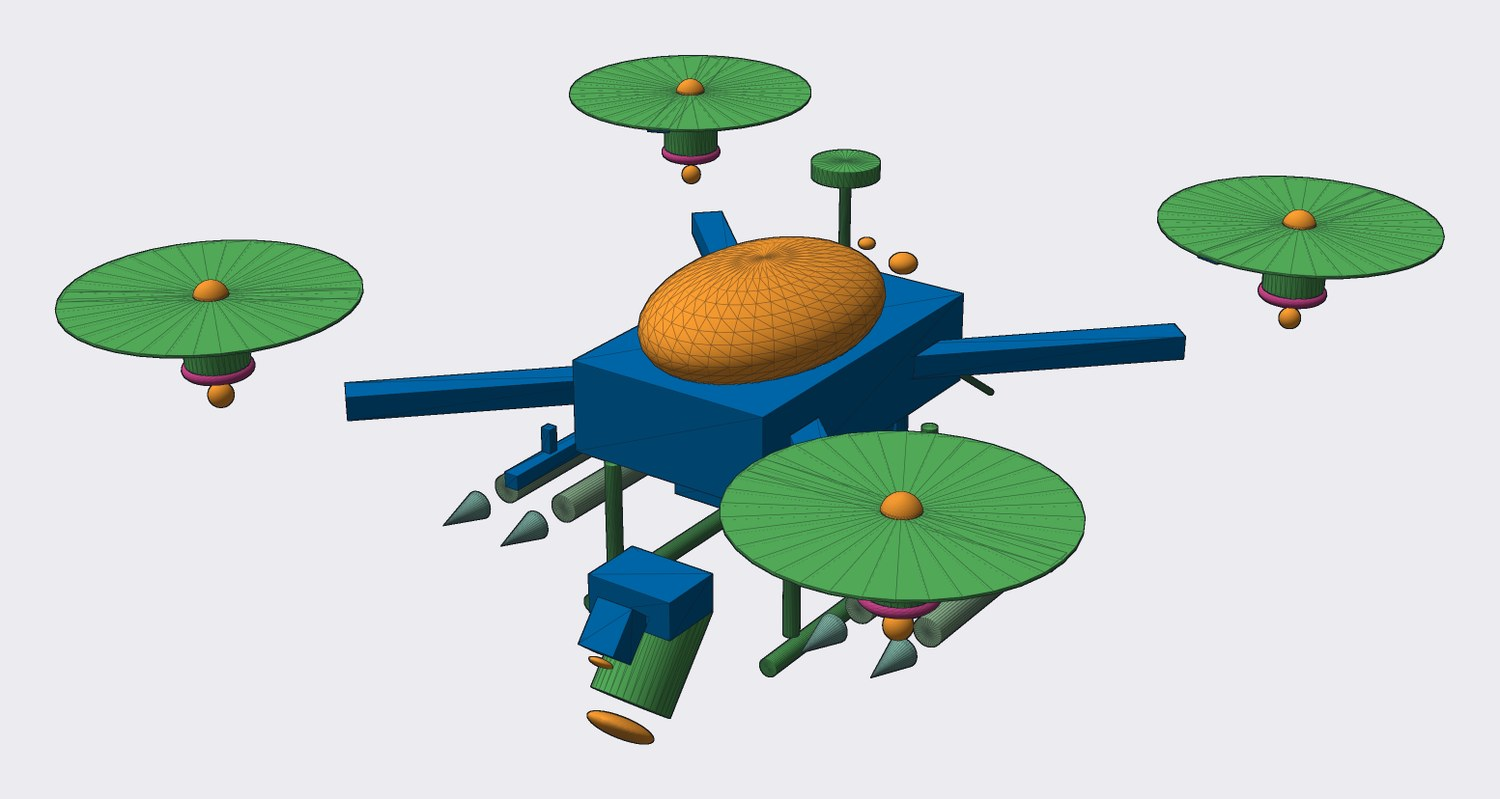
\includegraphics[width=7.00cm]{figures/img/shapes/autonomous_uav_prims.jpg}};
\node[anchor=west,inner sep=1pt] (L0) at (7.25,3.11) {Motor mount};
\draw[black!70,line width=0.4pt] (L0.west) -- (4.20,1.09); \fill[black] (4.20,1.09) circle (0.6pt);
\draw[black!70,line width=0.4pt] (L0.west) -- (1.01,2.13); \fill[black] (1.01,2.13) circle (0.6pt);
\draw[black!70,line width=0.4pt] (L0.west) -- (6.04,2.48); \fill[black] (6.04,2.48) circle (0.6pt);
\draw[black!70,line width=0.4pt] (L0.west) -- (3.22,3.12); \fill[black] (3.22,3.12) circle (0.6pt);
\node[anchor=west,inner sep=1pt] (L1) at (7.25,1.86) {Launcher rail};
\draw[black!70,line width=0.4pt] (L1.west) -- (2.78,1.68); \fill[black] (2.78,1.68) circle (0.6pt);
\draw[black!70,line width=0.4pt] (L1.west) -- (4.43,1.15); \fill[black] (4.43,1.15) circle (0.6pt);
\node[anchor=west,inner sep=1pt] (L2) at (7.25,0.62) {Gimbal yaw};
\draw[black!70,line width=0.4pt] (L2.west) -- (3.03,0.67); \fill[black] (3.03,0.67) circle (0.6pt);
\end{tikzpicture}\\[-0.3mm]{\fontsize{7.5}{9}\selectfont Full model} & {\fontsize{7.5}{9}\selectfont Made of primitives (pulled apart)}\end{tabular}
\\[0.8mm]{\fontsize{7}{8.5}\selectfont \primchipn{cuboid}{18}\quad \primchipn{sphere}{13}\quad \primchipn{cylinder}{19}\quad \primchipn{frustum}{1}\quad \primchipn{torus}{4}\quad \textbf{total 55}\\pale: UAV round $\times$4 (24 parts); $^\dagger$ 4 hidden at the start, drawn at rest scale on the right}\vspace{0.6mm}\end{minipage}}
\captionof{figure}{Autonomous UAV.}\label{fig:d-autonomous_uav}
\end{center}\vspace{-3mm}
\noindent\textbf{Autonomous UAV.}\label{des:autonomous_uav} Patrol quadcopter. 2 instances; the first stands 12\,m north of the bunker. Placement of the first: $T(0.00,\,7.50,\,12.50)\,R_y(-180^\circ)\,S(1)$.
{\fontsize{7}{8.2}\selectfont\setlength{\tabcolsep}{2.6pt}\renewcommand{\arraystretch}{1.02}
\begin{longtable}{@{}>{\raggedright\arraybackslash}p{3.3cm}l>{\raggedright\arraybackslash}p{2.7cm}>{\raggedright\arraybackslash}p{4.2cm}>{\raggedright\arraybackslash}p{2.3cm}>{\raggedright\arraybackslash}p{2.4cm}@{}}
\toprule Part ($\times n$) & Shape & Size $S$ (cm) & Position $T$ (cm, design frame) & Rotation $R$ ($^\circ$) & Parent\\\midrule\endhead
\bottomrule\endfoot
\multicolumn{6}{@{}l}{\textit{Autonomous UAV}}\\[0.2mm]
Fuselage & \primchip{cuboid} & $16{\times}7{\times}26$ & $(0,\,0,\,0)$ & -- & root\\
Canopy & \primchip{sphere} & $15{\times}8{\times}22$ & $(0,\,4,\,1)$ & -- & root\\
Battery & \primchip{cuboid} & $10{\times}4{\times}16$ & $(0,\,-5,\,-2)$ & -- & root\\
GPS mast & \primchip{cylinder} & $0.8{\times}0.8{\times}5$ & $(0,\,7,\,-7)$ & $(90,\,0,\,0)$ & root\\
GPS puck & \primchip{cylinder} & $5{\times}5{\times}1.2$ & $(0,\,10,\,-7)$ & $(90,\,0,\,0)$ & root\\
Arm Front-left & \primchip{cuboid} & $2.5{\times}1.8{\times}22$ & $(11,\,0,\,11)$ & $(0,\,45,\,0)$ & root\\
Arm Front-right & \primchip{cuboid} & $2.5{\times}1.8{\times}22$ & $(-11,\,0,\,11)$ & $(0,\,-45,\,0)$ & root\\
Arm Rear-left & \primchip{cuboid} & $2.5{\times}1.8{\times}22$ & $(11,\,0,\,-11)$ & $(0,\,135,\,0)$ & root\\
Arm Rear-right & \primchip{cuboid} & $2.5{\times}1.8{\times}22$ & $(-11,\,0,\,-11)$ & $(0,\,-135,\,0)$ & root\\
Strobe & \primchip{sphere} & $2.2{\times}1.6{\times}2.2$ & $(0,\,2,\,-14)$ & -- & root\\
Landing strut $\times$4 & \primchip{cylinder} & $1.2{\times}1.2{\times}9$ & $(\pm 6,\,-8,\,\pm 7)$ & $(90,\,0,\,0)$ & root\\
Landing skid $\times$2 & \primchip{cylinder} & $1.4{\times}1.4{\times}24$ & $(\pm 6,\,-12,\,0)$ & -- & root\\
Telemetry antenna $\times$2 & \primchip{cylinder} & $0.5{\times}0.5{\times}9$ & $(\pm 5,\,-4,\,-13)$ & $(-35,\,0,\,0)$ & root\\
Battery strap $\times$2 & \primchip{cuboid} & $10.6{\times}4.4{\times}1.2$ & $(0,\,-5,\,\{-7,3\})$ & -- & root\\
Arming LED & \primchip{sphere} & $1.2{\times}0.8{\times}1.2$ & $(4,\,7,\,-3)$ & -- & root\\
\multicolumn{6}{@{}l}{\textit{Motor mount}}\\[0.2mm]
Motor $\times$4 & \primchip{cylinder} & $4.5{\times}4.5{\times}3.5$ & $(\pm 18,\,3,\,\pm 18)$ & $(90,\,0,\,0)$ & Motor mount\\
Prop hub $\times$4 & \primchip{sphere} & $2.5{\times}2.5{\times}2.5$ & $(\pm 18,\,6,\,\pm 18)$ & -- & Rotor\\
Prop blade $\times$4\,$^\dagger$ & \primchip{cuboid} & $20{\times}0.4{\times}1.8$ & $(\pm 18,\,6,\,\pm 18)$ & -- & Rotor\\
Rotor blur disc $\times$4 & \primchip{cylinder} & $20.5{\times}20.5{\times}0.2$ & $(\pm 18,\,6,\,\pm 18)$ & $(90,\,0,\,0)$ & Motor mount\\
Nav LED $\times$2 & \primchip{sphere} & $1.8{\times}1.8{\times}1.8$ & $(\pm 18,\,0,\,18)$ & -- & Motor mount\\
Motor cooling ring $\times$4 & \primchip{torus} & $5{\times}5{\times}3.33$ & $(\pm 18,\,2,\,\pm 18)$ & $(90,\,0,\,0)$ & Motor mount\\
Status LED $\times$2 & \primchip{sphere} & $1.6{\times}1.6{\times}1.6$ & $(\pm 18,\,0,\,-18)$ & -- & Motor mount\\
\multicolumn{6}{@{}l}{\textit{Gimbal yaw}}\\[0.2mm]
Gimbal yoke & \primchip{cuboid} & $7{\times}3{\times}5$ & $(0,\,-7,\,10)$ & -- & Gimbal yaw\\
Lamp housing & \primchip{cylinder} & $6{\times}6{\times}8$ & $(0,\,-11,\,10)$ & -- & Gimbal pitch\\
Lens & \primchip{sphere} & $5{\times}5{\times}1.5$ & $(0,\,-14,\,13)$ & -- & Gimbal pitch\\
Thermal camera & \primchip{cuboid} & $3{\times}2.5{\times}3.5$ & $(0,\,-8,\,13)$ & -- & Gimbal pitch\\
Light cone & \primchip{frustum} & $486{\times}486{\times}974$ & $(0,\,-388,\,326)$ & -- & Gimbal pitch\\
Camera window & \primchip{sphere} & $1.8{\times}1.8{\times}0.6$ & $(0,\,-10,\,14)$ & -- & Gimbal pitch\\
\multicolumn{6}{@{}l}{\textit{Launcher rail}}\\[0.2mm]
Rail $\times$2 & \primchip{cuboid} & $1.2{\times}1.2{\times}22$ & $(\pm 10,\,-6,\,0)$ & -- & Launcher rail\\
Rail strut $\times$2 & \primchip{cuboid} & $0.8{\times}2{\times}0.8$ & $(\pm 10,\,-5,\,5)$ & -- & Launcher rail\\
\textit{UAV round} $\times$4 & \multicolumn{5}{@{}l}{\textit{nested design, drawn pale; its parts are counted in its own card (Figure~\ref{fig:d-uav_round})}}\\
\end{longtable}}
\uavextras

\needspace{8.6cm}
\begin{center}
\fcolorbox{black!30}{white}{\begin{minipage}{0.975\linewidth}\centering\vspace{0.6mm}
\begin{tabular}{@{}c@{\hspace{3mm}}c@{}}\img{figures/img/shapes/cargo_truck_model.jpg}{4.33cm} & \img{figures/img/shapes/cargo_truck_prims.jpg}{4.42cm}\\[-0.3mm]{\fontsize{7.5}{9}\selectfont Full model} & {\fontsize{7.5}{9}\selectfont Made of primitives (pulled apart)}\end{tabular}
\\[0.8mm]{\fontsize{7}{8.5}\selectfont \primchipn{cuboid}{15}\quad \primchipn{sphere}{2}\quad \primchipn{cylinder}{14}\quad \textbf{total 31}}\vspace{0.6mm}\end{minipage}}
\captionof{figure}{Cargo truck.}\label{fig:d-cargo_truck}
\end{center}\vspace{-3mm}
\noindent\textbf{Cargo truck.}\label{des:cargo_truck} 6x6 tactical truck, parked (local +Z = front). 2 instances; the first stands 26\,m south-west of the bunker, inside the motor pool. Placement of the first: $T(-15.64,\,-0.30,\,-20.38)\,R_y(45^\circ)\,S(1)$.
{\fontsize{7}{8.2}\selectfont\setlength{\tabcolsep}{2.6pt}\renewcommand{\arraystretch}{1.02}
\begin{longtable}{@{}>{\raggedright\arraybackslash}p{3.3cm}l>{\raggedright\arraybackslash}p{2.7cm}>{\raggedright\arraybackslash}p{4.2cm}>{\raggedright\arraybackslash}p{2.3cm}>{\raggedright\arraybackslash}p{2.4cm}@{}}
\toprule Part ($\times n$) & Shape & Size $S$ (cm) & Position $T$ (cm, design frame) & Rotation $R$ ($^\circ$) & Parent\\\midrule\endhead
\bottomrule\endfoot
Chassis & \primchip{cuboid} & $100{\times}30{\times}700$ & $(0,\,75,\,-30)$ & -- & root\\
Hood & \primchip{cuboid} & $200{\times}95{\times}160$ & $(0,\,145,\,290)$ & -- & root\\
Cab & \primchip{cuboid} & $235{\times}155{\times}150$ & $(0,\,185,\,135)$ & -- & root\\
Windscreen & \primchip{cuboid} & $200{\times}70{\times}4$ & $(0,\,210,\,212)$ & -- & root\\
Bumper & \primchip{cuboid} & $230{\times}25{\times}30$ & $(0,\,85,\,380)$ & -- & root\\
Cargo bed & \primchip{cuboid} & $240{\times}20{\times}420$ & $(0,\,125,\,-165)$ & -- & root\\
Bed side $\times$2 & \primchip{cuboid} & $8{\times}55{\times}420$ & $(\pm 120,\,160,\,-165)$ & -- & root\\
Canvas cover & \primchip{cylinder} & $230{\times}190{\times}400$ & $(0,\,195,\,-165)$ & -- & root\\
Wheel $\times$6 & \primchip{cylinder} & $105{\times}105{\times}40$ & $(\pm 110,\,53,\,\{-270,-120,275\})$ & $(0,\,90,\,0)$ & root\\
Fender $\times$2 & \primchip{cuboid} & $25{\times}10{\times}130$ & $(\pm 110,\,112,\,275)$ & -- & root\\
Headlight $\times$2 & \primchip{sphere} & $22{\times}22{\times}10$ & $(\pm 70,\,155,\,372)$ & -- & root\\
Wheel hub $\times$6 & \primchip{cylinder} & $45{\times}45{\times}42$ & $(\pm 110,\,53,\,\{-270,-120,275\})$ & $(0,\,90,\,0)$ & root\\
Cab side window $\times$2 & \primchip{cuboid} & $2{\times}50{\times}70$ & $(\pm 118,\,220,\,140)$ & -- & root\\
Mirror $\times$2 & \primchip{cuboid} & $5{\times}30{\times}18$ & $(\pm 132,\,220,\,195)$ & -- & root\\
Radiator grille & \primchip{cuboid} & $100{\times}60{\times}2$ & $(0,\,145,\,371)$ & -- & root\\
Exhaust stack & \primchip{cylinder} & $12{\times}12{\times}100$ & $(105,\,250,\,50)$ & $(90,\,0,\,0)$ & root\\
\end{longtable}}

\needspace{8.6cm}
\begin{center}
\fcolorbox{black!30}{white}{\begin{minipage}{0.975\linewidth}\centering\vspace{0.6mm}
\begin{tabular}{@{}c@{\hspace{3mm}}c@{}}\img{figures/img/shapes/target_rover_model.jpg}{3.38cm} & \img{figures/img/shapes/target_rover_prims.jpg}{3.45cm}\\[-0.3mm]{\fontsize{7.5}{9}\selectfont Full model} & {\fontsize{7.5}{9}\selectfont Made of primitives (pulled apart)}\end{tabular}
\\[0.8mm]{\fontsize{7}{8.5}\selectfont \primchipn{cuboid}{6}\quad \primchipn{sphere}{12}\quad \primchipn{cylinder}{8}\quad \textbf{total 26}}\vspace{0.6mm}\end{minipage}}
\captionof{figure}{Target rover.}\label{fig:d-target_rover}
\end{center}\vspace{-3mm}
\noindent\textbf{Target rover.}\label{des:target_rover} Ground robot hiding from the UAV. 6 instances; the first stands 10\,m north-east of the bunker. Placement of the first: $T(6.00,\,0.14,\,7.50)\,R_y(0^\circ)\,S(1)$.
{\fontsize{7}{8.2}\selectfont\setlength{\tabcolsep}{2.6pt}\renewcommand{\arraystretch}{1.02}
\begin{longtable}{@{}>{\raggedright\arraybackslash}p{3.3cm}l>{\raggedright\arraybackslash}p{2.7cm}>{\raggedright\arraybackslash}p{4.2cm}>{\raggedright\arraybackslash}p{2.3cm}>{\raggedright\arraybackslash}p{2.4cm}@{}}
\toprule Part ($\times n$) & Shape & Size $S$ (cm) & Position $T$ (cm, design frame) & Rotation $R$ ($^\circ$) & Parent\\\midrule\endhead
\bottomrule\endfoot
\multicolumn{6}{@{}l}{\textit{Target rover}}\\[0.2mm]
Chassis & \primchip{cuboid} & $42{\times}10{\times}62$ & $(0,\,14,\,0)$ & -- & root\\
Upper hull & \primchip{cuboid} & $34{\times}10{\times}40$ & $(0,\,24,\,-4)$ & -- & root\\
Motor + battery box & \primchip{cuboid} & $22{\times}7{\times}16$ & $(0,\,33,\,-14)$ & -- & root\\
Front bumper & \primchip{cuboid} & $44{\times}5{\times}4$ & $(0,\,12,\,33)$ & -- & root\\
Wheel $\times$6 & \primchip{cylinder} & $16{\times}16{\times}7$ & $(\pm 25,\,8,\,-22{+}22i)$ & $(0,\,90,\,0)$ & root\\
Hub $\times$6 & \primchip{sphere} & $7{\times}7{\times}3$ & $(\pm 29,\,8,\,-22{+}22i)$ & $(0,\,90,\,0)$ & root\\
IR sensor bar & \primchip{cuboid} & $30{\times}2{\times}4$ & $(0,\,7,\,30)$ & -- & root\\
IR sensor $\times$5 & \primchip{sphere} & $2.5{\times}2.5{\times}2.5$ & $(\pm(0{+}6i),\,\{5,6\},\,31)$ & -- & root\\
Sensor mast & \primchip{cylinder} & $2.5{\times}2.5{\times}16$ & $(8,\,37,\,10)$ & $(90,\,0,\,0)$ & root\\
Whip antenna & \primchip{cylinder} & $1.2{\times}1.2{\times}30$ & $(-13,\,44,\,-20)$ & $(90,\,0,\,0)$ & root\\
\multicolumn{6}{@{}l}{\textit{Scanner pivot}}\\[0.2mm]
Scanner head & \primchip{sphere} & $7{\times}7{\times}7$ & $(8,\,46,\,10)$ & -- & Scanner pivot\\
Scanner window & \primchip{cuboid} & $5{\times}3{\times}2$ & $(8,\,46,\,13)$ & -- & Scanner pivot\\
\end{longtable}}
\FloatBarrier}
\newcommand{\designcardsWeaponsAndMunitions}{%
\needspace{10.6cm}
\begin{center}
\fcolorbox{black!30}{white}{\begin{minipage}{0.975\linewidth}\centering\vspace{0.6mm}
\begin{tabular}{@{}c@{\hspace{3mm}}c@{}}\img{figures/img/shapes/sam_launcher_model.jpg}{6.75cm} & \begin{tikzpicture}[font=\fontsize{7}{8}\selectfont]
\node[inner sep=0,anchor=south west] at (0,0) {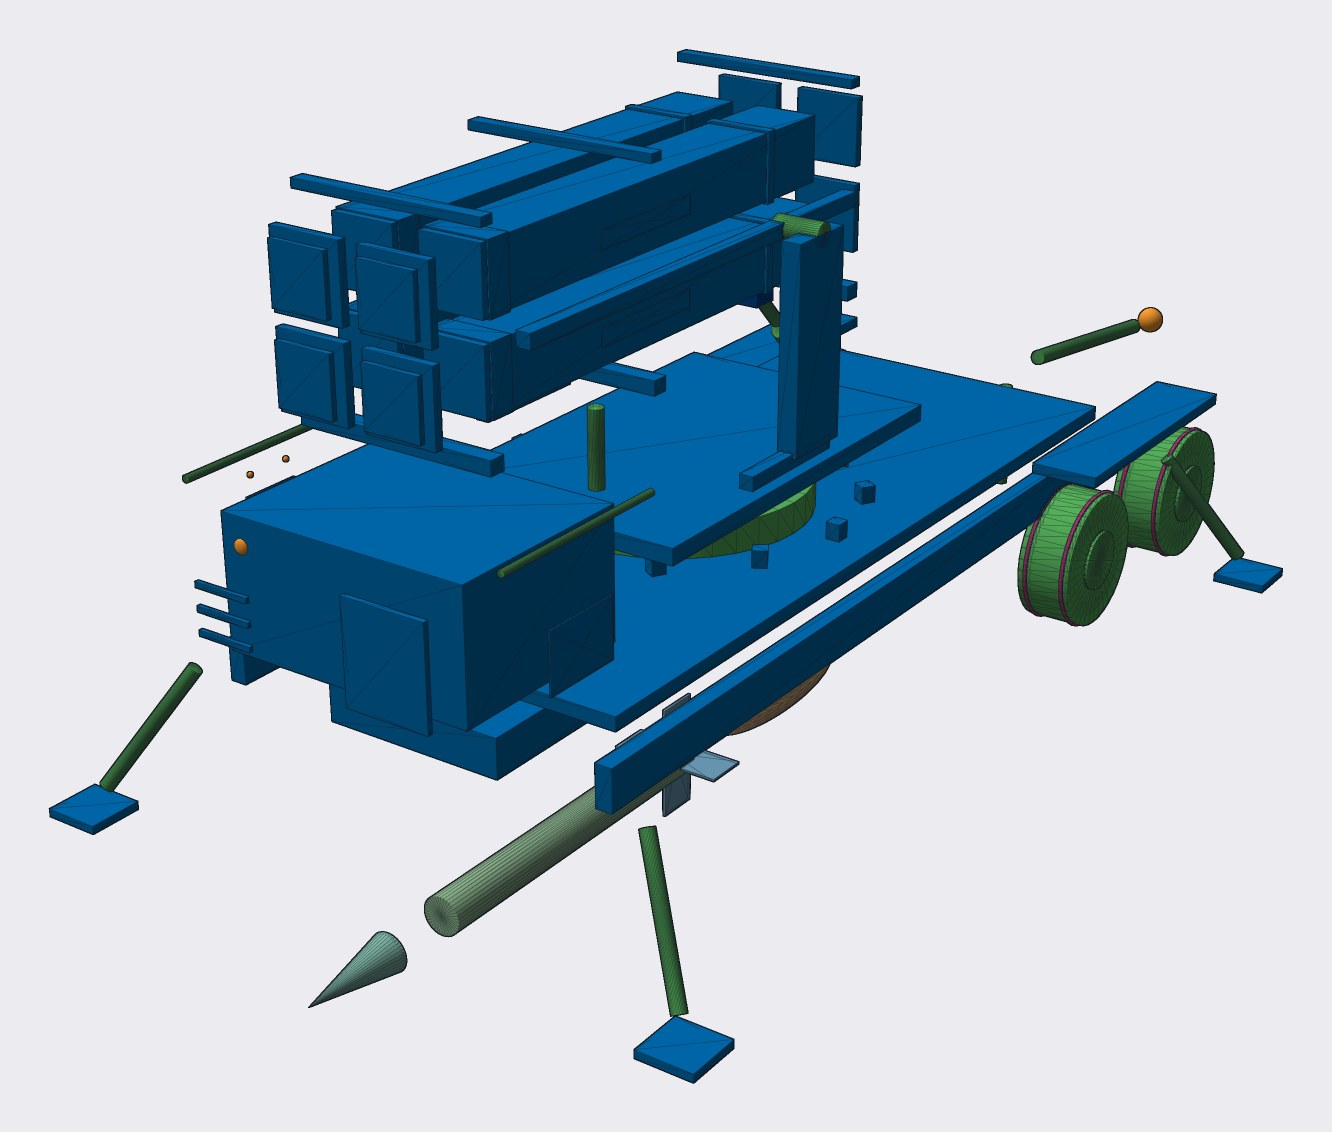
\includegraphics[width=6.59cm]{figures/img/shapes/sam_launcher_prims.jpg}};
\node[anchor=west,inner sep=1pt] (L0) at (6.84,4.67) {Canister};
\draw[black!70,line width=0.4pt] (L0.west) -- (2.72,4.68); \fill[black] (2.72,4.68) circle (0.6pt);
\draw[black!70,line width=0.4pt] (L0.west) -- (3.14,4.60); \fill[black] (3.14,4.60) circle (0.6pt);
\draw[black!70,line width=0.4pt] (L0.west) -- (2.73,4.22); \fill[black] (2.73,4.22) circle (0.6pt);
\draw[black!70,line width=0.4pt] (L0.west) -- (3.14,4.13); \fill[black] (3.14,4.13) circle (0.6pt);
\node[anchor=west,inner sep=1pt] (L1) at (6.84,2.80) {Trailer};
\draw[black!70,line width=0.4pt] (L1.west) -- (3.63,3.41); \fill[black] (3.63,3.41) circle (0.6pt);
\node[anchor=west,inner sep=1pt] (L2) at (6.84,0.93) {SAM round};
\draw[black!70,line width=0.4pt] (L2.west) -- (3.02,1.63); \fill[black] (3.02,1.63) circle (0.6pt);
\end{tikzpicture}\\[-0.3mm]{\fontsize{7.5}{9}\selectfont Full model} & {\fontsize{7.5}{9}\selectfont Made of primitives (pulled apart)}\end{tabular}
\\[0.8mm]{\fontsize{7}{8.5}\selectfont \primchipn{cube}{1}\quad \primchipn{cuboid}{71}\quad \primchipn{sphere}{4}\quad \primchipn{cylinder}{23}\quad \primchipn{torus}{8}\quad \textbf{total 107}\\pale: SAM missile $\times$1 (5 parts)}\vspace{0.6mm}\end{minipage}}
\captionof{figure}{SAM launcher.}\label{fig:d-sam_launcher}
\end{center}\vspace{-3mm}
\noindent\textbf{SAM launcher.}\label{des:sam_launcher} Trailer-mounted surface-to-air missile launcher with four canisters (user controlled). One instance, 26\,m east of the bunker. Placement of the first: $T(25.10,\,-0.30,\,6.70)\,R_y(60^\circ)\,S(1)$.
{\fontsize{7}{8.2}\selectfont\setlength{\tabcolsep}{2.6pt}\renewcommand{\arraystretch}{1.02}
\begin{longtable}{@{}>{\raggedright\arraybackslash}p{3.3cm}l>{\raggedright\arraybackslash}p{2.7cm}>{\raggedright\arraybackslash}p{4.2cm}>{\raggedright\arraybackslash}p{2.3cm}>{\raggedright\arraybackslash}p{2.4cm}@{}}
\toprule Part ($\times n$) & Shape & Size $S$ (cm) & Position $T$ (cm, design frame) & Rotation $R$ ($^\circ$) & Parent\\\midrule\endhead
\bottomrule\endfoot
\multicolumn{6}{@{}l}{\textit{Trailer}}\\[0.2mm]
Trailer frame & \primchip{cuboid} & $130{\times}28{\times}680$ & $(0,\,86,\,0)$ & -- & Trailer\\
Trailer side rail $\times$2 & \primchip{cuboid} & $12{\times}30{\times}680$ & $(\pm 110,\,90,\,0)$ & -- & Trailer\\
Trailer deck & \primchip{cuboid} & $260{\times}10{\times}620$ & $(0,\,109,\,0)$ & -- & Trailer\\
Wheel $\times$4 & \primchip{cylinder} & $100{\times}100{\times}40$ & $(\pm 125,\,50,\,\{-290,-170\})$ & $(0,\,90,\,0)$ & Trailer\\
Wheel hub $\times$4 & \primchip{cylinder} & $45{\times}45{\times}44$ & $(\pm 125,\,50,\,\{-290,-170\})$ & $(0,\,90,\,0)$ & Trailer\\
Fender $\times$2 & \primchip{cuboid} & $50{\times}8{\times}210$ & $(\pm 125,\,105,\,-230)$ & -- & Trailer\\
Tow bar & \primchip{cylinder} & $12{\times}12{\times}192$ & $(0,\,77,\,-435)$ & $(7,\,180,\,0)$ & Trailer\\
Tow eye & \primchip{sphere} & $22{\times}22{\times}22$ & $(0,\,65,\,-535)$ & -- & Trailer\\
Landing leg & \primchip{cylinder} & $10{\times}10{\times}85$ & $(0,\,47,\,-320)$ & $(90,\,0,\,0)$ & Trailer\\
Outrigger $\times$4 & \primchip{cylinder} & $10{\times}10{\times}106$ & $(\pm 155,\,48,\,\pm 280)$ & $(53,\,\pm(51{+}78i),\,0)$ & Trailer\\
Outrigger pad $\times$4 & \primchip{cuboid} & $40{\times}6{\times}40$ & $(\pm 180,\,3,\,\pm 300)$ & -- & Trailer\\
Control cabin & \primchip{cuboid} & $180{\times}90{\times}140$ & $(0,\,159,\,250)$ & -- & Trailer\\
Cabin door & \primchip{cuboid} & $60{\times}70{\times}4$ & $(40,\,155,\,321)$ & -- & Trailer\\
Cabin louvre $\times$3 & \primchip{cuboid} & $40{\times}4{\times}3$ & $(-55,\,140{+}12i,\,321)$ & -- & Trailer\\
Cabin exhaust & \primchip{cylinder} & $10{\times}10{\times}50$ & $(70,\,225,\,210)$ & $(90,\,0,\,0)$ & Trailer\\
Cabin tactical lamp & \primchip{sphere} & $10{\times}10{\times}5$ & $(-40,\,190,\,322)$ & -- & Trailer\\
Power cable & \primchip{cylinder} & $7{\times}7{\times}90$ & $(0,\,121,\,135)$ & $(-1,\,180,\,0)$ & Trailer\\
Status panel & \primchip{cuboid} & $1.2{\times}26{\times}42$ & $(-91,\,172,\,250)$ & -- & Trailer\\
Status LED $\times$2 & \primchip{sphere} & $4{\times}4{\times}4$ & $(-91,\,192,\,\{238,262\})$ & -- & Trailer\\
Generator grille & \primchip{cuboid} & $1.2{\times}42{\times}60$ & $(91,\,150,\,250)$ & -- & Trailer\\
Cabin roof edge $\times$2 & \primchip{cylinder} & $5{\times}5{\times}140$ & $(\pm 90,\,204,\,250)$ & -- & Trailer\\
Tyre tread $\times$8 & \primchip{torus} & $103{\times}103{\times}26.7$ & $(\pm(114{+}22i),\,50,\,\{-290,-170\})$ & $(0,\,90,\,0)$ & Trailer\\
\multicolumn{6}{@{}l}{\textit{Turntable}}\\[0.2mm]
Slew ring & \primchip{cylinder} & $190{\times}190{\times}22$ & $(0,\,125,\,40)$ & $(90,\,0,\,0)$ & Turntable\\
Slew gear tooth $\times$12 & \primchip{cuboid} & $10{\times}12{\times}10$ & $(-98..98,\,125,\,-58..138)$ & $(0,\,-330{+}30i,\,0)$ & Turntable\\
Turntable deck & \primchip{cuboid} & $190{\times}12{\times}300$ & $(0,\,142,\,30)$ & -- & Turntable\\
Cradle upright $\times$2 & \primchip{cuboid} & $14{\times}140{\times}50$ & $(\pm 80,\,219,\,40)$ & -- & Turntable\\
Upright brace $\times$2 & \primchip{cuboid} & $10{\times}10{\times}90$ & $(\pm 80,\,164,\,60)$ & -- & Turntable\\
Ram foot & \primchip{cuboid} & $30{\times}16{\times}30$ & $(0,\,148,\,-90)$ & -- & Turntable\\
Ram cylinder & \primchip{cylinder} & $16{\times}16{\times}47.5$ & $(0,\,169,\,-73)$ & $(-46,\,0,\,0)$ & Turntable\\
Ram rod & \primchip{cylinder} & $9{\times}9{\times}43.1$ & $(0,\,198,\,-45)$ & $(-46,\,0,\,0)$ & Turntable\\
Cradle rail $\times$2 & \primchip{cuboid} & $10{\times}10{\times}340$ & $(\pm 62,\,274,\,110)$ & -- & Cradle\\
Trunnion $\times$2 & \primchip{cylinder} & $16{\times}16{\times}34$ & $(\pm 72,\,274,\,40)$ & $(0,\,90,\,0)$ & Cradle\\
Cradle cross beam $\times$3 & \primchip{cuboid} & $140{\times}10{\times}12$ & $(0,\,219,\,\{-40,130,250\})$ & -- & Cradle\\
Canister strap $\times$3 & \primchip{cuboid} & $135{\times}6{\times}10$ & $(0,\,326,\,\{-40,130,250\})$ & -- & Cradle\\
Ram lug & \primchip{cube} & $20{\times}20{\times}20$ & $(0,\,214,\,-30)$ & -- & Cradle\\
Canister tube $\times$4 & \primchip{cuboid} & $44{\times}44{\times}340$ & $(\pm 28,\,\{248,300\},\,110)$ & -- & Canister\\
Hazard band $\times$4 & \primchip{cuboid} & $46{\times}46{\times}18$ & $(\pm 28,\,\{248,300\},\,230)$ & -- & Canister\\
Muzzle collar $\times$4 & \primchip{cuboid} & $50{\times}50{\times}6$ & $(\pm 28,\,\{248,300\},\,275)$ & -- & Canister\\
Canister cap $\times$4 & \primchip{cuboid} & $40{\times}40{\times}4$ & $(\pm 28,\,\{248,300\},\,281)$ & -- & Canister\\
Rear hatch $\times$4 & \primchip{cuboid} & $46{\times}46{\times}6$ & $(\pm 28,\,\{248,300\},\,-62)$ & -- & Canister\\
Canister rib $\times$4 & \primchip{cuboid} & $47{\times}47{\times}7$ & $(\pm 28,\,\{248,300\},\,20)$ & -- & Canister\\
Canister stencil $\times$4 & \primchip{cuboid} & $0.6{\times}12{\times}90$ & $(\pm 50,\,\{248,300\},\,130)$ & -- & Canister\\
\multicolumn{6}{@{}l}{\textit{SAM launcher}}\\[0.2mm]
\textit{SAM missile} $\times$1 & \multicolumn{5}{@{}l}{\textit{nested design, drawn pale; its parts are counted in its own card (Figure~\ref{fig:d-sam_missile})}}\\
\end{longtable}}

\needspace{10.6cm}
\begin{center}
\fcolorbox{black!30}{white}{\begin{minipage}{0.975\linewidth}\centering\vspace{0.6mm}
\begin{tabular}{@{}c@{\hspace{3mm}}c@{}}\img{figures/img/shapes/aa_gatling_gun_model.jpg}{6.10cm} & \begin{tikzpicture}[font=\fontsize{7}{8}\selectfont]
\node[inner sep=0,anchor=south west] at (0,0) {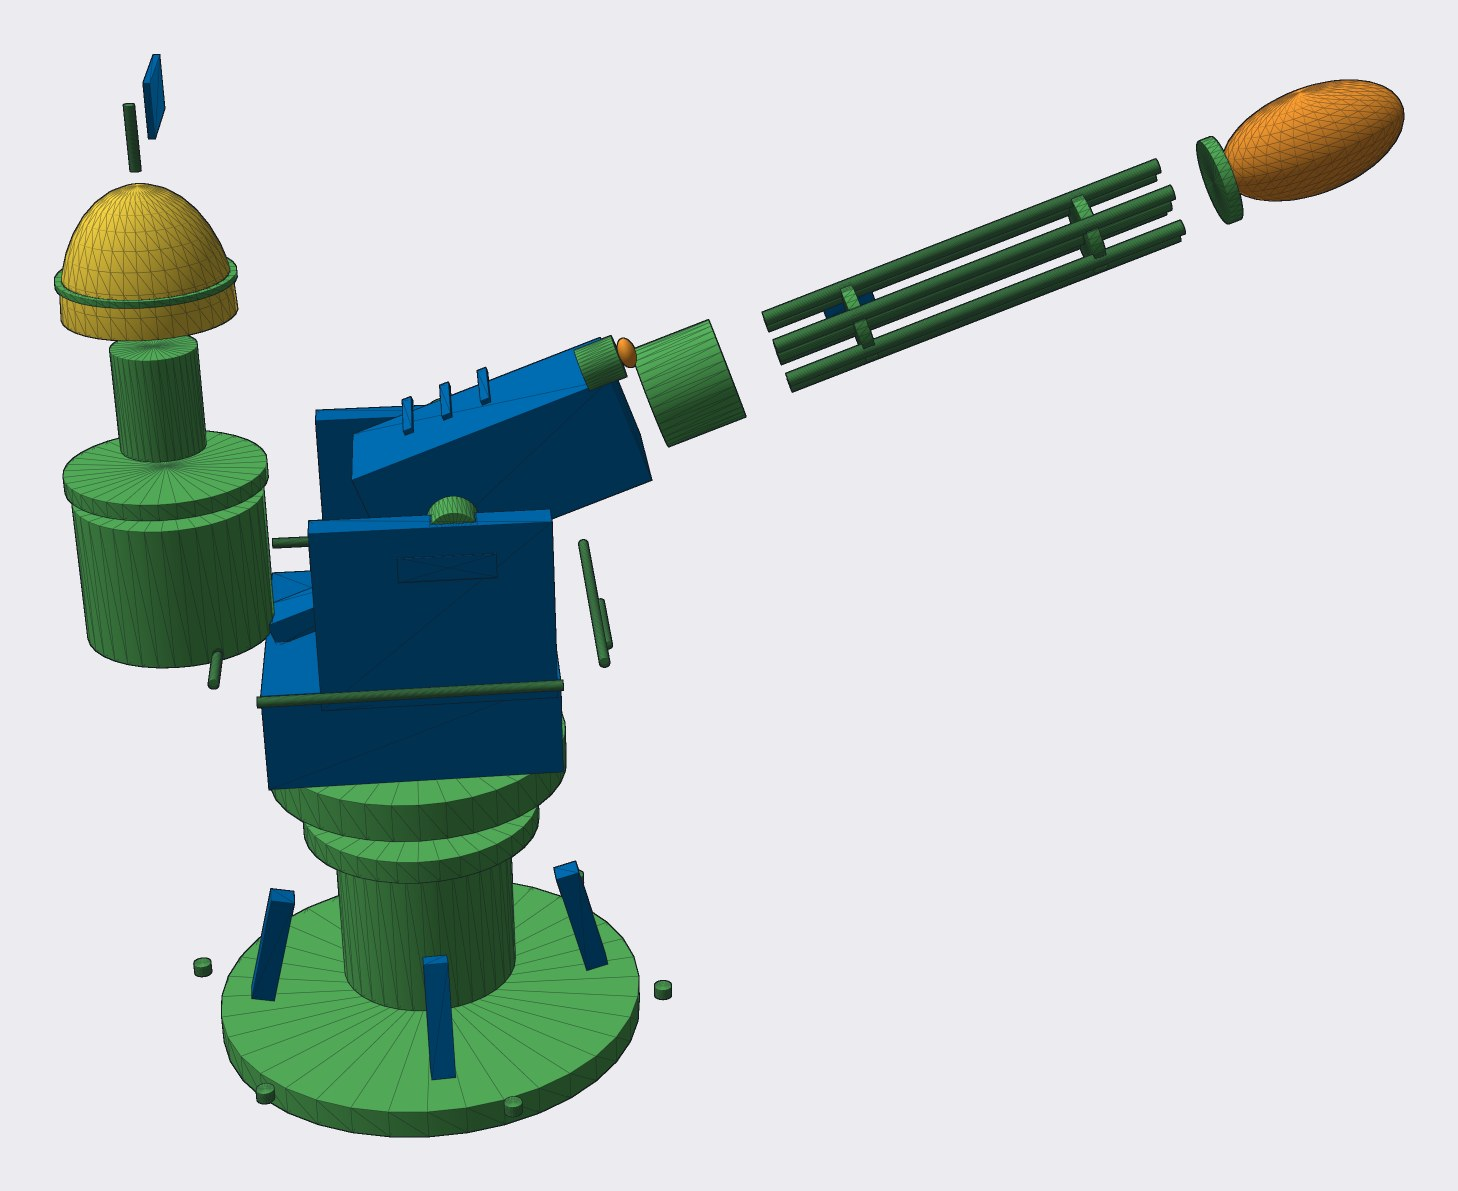
\includegraphics[width=6.86cm]{figures/img/shapes/aa_gatling_gun_prims.jpg}};
\node[anchor=west,inner sep=1pt] (L0) at (7.11,2.80) {Barrel cluster};
\draw[black!70,line width=0.4pt] (L0.west) -- (4.63,4.32); \fill[black] (4.63,4.32) circle (0.6pt);
\end{tikzpicture}\\[-0.3mm]{\fontsize{7.5}{9}\selectfont Full model} & {\fontsize{7.5}{9}\selectfont Made of primitives (pulled apart)}\end{tabular}
\\[0.8mm]{\fontsize{7}{8.5}\selectfont \primchipn{cuboid}{19}\quad \primchipn{sphere}{4}\quad \primchipn{hemisphere}{1}\quad \primchipn{cylinder}{34}\quad \textbf{total 58}\\pale: AA shell casing $\times$20 (20 parts); $^\dagger$ 1 hidden at the start, drawn at rest scale on the right; 20 parked below ground, not drawn}\vspace{0.6mm}\end{minipage}}
\captionof{figure}{AA Gatling gun.}\label{fig:d-aa_gatling_gun}
\end{center}\vspace{-3mm}
\noindent\textbf{AA Gatling gun.}\label{des:aa_gatling_gun} User-controllable anti-aircraft Gatling gun with radar dome. One instance, 28\,m south-east of the bunker. Placement of the first: $T(21.00,\,-0.30,\,-19.00)\,R_y(0^\circ)\,S(1)$.
{\fontsize{7}{8.2}\selectfont\setlength{\tabcolsep}{2.6pt}\renewcommand{\arraystretch}{1.02}
\begin{longtable}{@{}>{\raggedright\arraybackslash}p{3.3cm}l>{\raggedright\arraybackslash}p{2.7cm}>{\raggedright\arraybackslash}p{4.2cm}>{\raggedright\arraybackslash}p{2.3cm}>{\raggedright\arraybackslash}p{2.4cm}@{}}
\toprule Part ($\times n$) & Shape & Size $S$ (cm) & Position $T$ (cm, design frame) & Rotation $R$ ($^\circ$) & Parent\\\midrule\endhead
\bottomrule\endfoot
\multicolumn{6}{@{}l}{\textit{AA Gatling gun}}\\[0.2mm]
Base plate & \primchip{cylinder} & $220{\times}220{\times}15$ & $(0,\,8,\,0)$ & $(90,\,0,\,0)$ & root\\
Pedestal column & \primchip{cylinder} & $90{\times}90{\times}85$ & $(0,\,57,\,0)$ & $(90,\,0,\,0)$ & root\\
Pedestal collar & \primchip{cylinder} & $120{\times}120{\times}12$ & $(0,\,95,\,0)$ & $(90,\,0,\,0)$ & root\\
Pedestal brace $\times$4 & \primchip{cuboid} & $12{\times}60{\times}12$ & $(\pm 44,\,40,\,\pm 44)$ & $(-14,\,45{+}90i,\,0)$ & root\\
Anchor bolt $\times$6 & \primchip{cylinder} & $9{\times}9{\times}6$ & $(-82{+}82i,\,17,\,\pm(48{+}47i))$ & $(90,\,0,\,0)$ & root\\
\textit{AA shell casing} $\times$20 & \multicolumn{5}{@{}l}{\textit{nested design, drawn pale; its parts are counted in its own card (Figure~\ref{fig:d-aa_shell_casing})}}\\
\multicolumn{6}{@{}l}{\textit{Mount yaw}}\\[0.2mm]
Turntable & \primchip{cylinder} & $150{\times}150{\times}20$ & $(0,\,115,\,0)$ & $(90,\,0,\,0)$ & Mount yaw\\
Mount body & \primchip{cuboid} & $140{\times}50{\times}140$ & $(0,\,150,\,0)$ & -- & Mount yaw\\
Cheek $\times$2 & \primchip{cuboid} & $15{\times}90{\times}110$ & $(\{-29,44\},\,200,\,\{-47,34\})$ & -- & Mount yaw\\
Ammo drum & \primchip{cylinder} & $90{\times}90{\times}70$ & $(-63,\,200,\,57)$ & $(90,\,0,\,0)$ & Mount yaw\\
Ammo drum lid & \primchip{cylinder} & $95{\times}95{\times}8$ & $(-63,\,235,\,57)$ & $(90,\,0,\,0)$ & Mount yaw\\
Radome mast & \primchip{cylinder} & $40{\times}40{\times}50$ & $(-63,\,265,\,57)$ & $(90,\,0,\,0)$ & Mount yaw\\
Radome & \primchip{hemisphere} & $80{\times}60{\times}80$ & $(-63,\,320,\,57)$ & -- & Mount yaw\\
Antenna mast & \primchip{cylinder} & $5{\times}5{\times}30$ & $(-63,\,360,\,57)$ & $(90,\,0,\,0)$ & Mount yaw\\
Search antenna plate & \primchip{cuboid} & $55{\times}25{\times}3$ & $(-70,\,377,\,50)$ & -- & Search antenna\\
Gun housing & \primchip{cuboid} & $60{\times}55{\times}130$ & $(29,\,237,\,-26)$ & -- & Cradle pitch\\
Trunnion $\times$2 & \primchip{cylinder} & $25{\times}25{\times}20$ & $(\{-19,48\},\,230,\,\{-50,24\})$ & $(0,\,90,\,0)$ & Cradle pitch\\
Front shroud & \primchip{cylinder} & $50{\times}50{\times}40$ & $(81,\,262,\,-73)$ & -- & Cradle pitch\\
Feed chute & \primchip{cuboid} & $25{\times}12{\times}90$ & $(-12,\,185,\,11)$ & -- & Cradle pitch\\
Ejection port & \primchip{cuboid} & $10{\times}12{\times}20$ & $(-3,\,245,\,-41)$ & -- & Cradle pitch\\
EO sensor pod & \primchip{cylinder} & $20{\times}20{\times}18$ & $(83,\,287,\,-18)$ & -- & Cradle pitch\\
EO sensor lens & \primchip{sphere} & $14{\times}14{\times}8$ & $(90,\,290,\,-25)$ & -- & Cradle pitch\\
Gatling barrel $\times$6 & \primchip{cylinder} & $7{\times}7{\times}200$ & $(155..175,\,290..317,\,-160..-138)$ & -- & Barrel cluster\\
Cluster shaft & \primchip{cylinder} & $10{\times}10{\times}200$ & $(165,\,304,\,-149)$ & -- & Barrel cluster\\
Barrel clamp rear & \primchip{cylinder} & $40{\times}40{\times}6$ & $(133,\,288,\,-121)$ & -- & Barrel cluster\\
Barrel clamp mid & \primchip{cylinder} & $40{\times}40{\times}6$ & $(196,\,319,\,-177)$ & -- & Barrel cluster\\
Barrel clamp muzzle & \primchip{cylinder} & $42{\times}42{\times}6$ & $(232,\,337,\,-210)$ & -- & Barrel cluster\\
Rotation marker & \primchip{cuboid} & $5{\times}5{\times}25$ & $(119,\,288,\,-136)$ & -- & Barrel cluster\\
Muzzle flash\,$^\dagger$ & \primchip{sphere} & $50{\times}50{\times}90$ & $(252,\,346,\,-228)$ & -- & Cradle pitch\\
Housing vent $\times$3 & \primchip{cuboid} & $42{\times}2.5{\times}4.5$ & $(4{+}11i,\,255{+}5i,\,-23{+}10i)$ & -- & Cradle pitch\\
Radome seam & \primchip{cylinder} & $82{\times}82{\times}3$ & $(-63,\,310,\,57)$ & $(90,\,0,\,0)$ & Mount yaw\\
Fire-control console & \primchip{cuboid} & $7{\times}34{\times}46$ & $(-27,\,155,\,-75)$ & -- & Mount yaw\\
Fire-control display & \primchip{cuboid} & $1{\times}22{\times}32$ & $(-30,\,157,\,-77)$ & -- & Mount yaw\\
Ready LED & \primchip{sphere} & $3.5{\times}3.5{\times}3.5$ & $(-38,\,175,\,-69)$ & -- & Mount yaw\\
Armed LED & \primchip{sphere} & $3.5{\times}3.5{\times}3.5$ & $(-21,\,175,\,-85)$ & -- & Mount yaw\\
Danger stencil $\times$2 & \primchip{cuboid} & $1{\times}12{\times}45$ & $(\{-31,54\},\,220,\,\{-57,37\})$ & -- & Mount yaw\\
Mount body edge $\times$4 & \primchip{cylinder} & $5{\times}5{\times}140$ & $(\pm(47{+}5i),\,175,\,\pm(47{+}5i))$ & $(0,\,\{0,90\},\,0)$ & Mount yaw\\
Grab handle & \primchip{cylinder} & $4{\times}4{\times}50$ & $(55,\,165,\,-50)$ & $(0,\,90,\,0)$ & Mount yaw\\
\end{longtable}}

\needspace{8.6cm}
\begin{center}
\fcolorbox{black!30}{white}{\begin{minipage}{0.975\linewidth}\centering\vspace{0.6mm}
\begin{tabular}{@{}c@{\hspace{3mm}}c@{}}\img{figures/img/shapes/sam_missile_model.jpg}{5.55cm} & \img{figures/img/shapes/sam_missile_prims.jpg}{5.57cm}\\[-0.3mm]{\fontsize{7.5}{9}\selectfont Full model} & {\fontsize{7.5}{9}\selectfont Made of primitives (pulled apart)}\end{tabular}
\\[0.8mm]{\fontsize{7}{8.5}\selectfont \primchipn{cuboid}{2}\quad \primchipn{sphere}{1}\quad \primchipn{cylinder}{1}\quad \primchipn{cone}{1}\quad \textbf{total 5}\\$^\dagger$ 5 hidden at the start, drawn at rest scale on the right}\vspace{0.6mm}\end{minipage}}
\captionof{figure}{SAM missile.}\label{fig:d-sam_missile}
\end{center}\vspace{-3mm}
\noindent\textbf{SAM missile.}\label{des:sam_missile} Flying round of the launch effect (hidden while in the canister). One instance, 26\,m east of the bunker, inside the sam launcher. Placement of the first: $T(25.10,\,-0.30,\,6.70)\,R_y(60^\circ)\,S(1)$.
{\fontsize{7}{8.2}\selectfont\setlength{\tabcolsep}{2.6pt}\renewcommand{\arraystretch}{1.02}
\begin{longtable}{@{}>{\raggedright\arraybackslash}p{3.3cm}l>{\raggedright\arraybackslash}p{2.7cm}>{\raggedright\arraybackslash}p{4.2cm}>{\raggedright\arraybackslash}p{2.3cm}>{\raggedright\arraybackslash}p{2.4cm}@{}}
\toprule Part ($\times n$) & Shape & Size $S$ (cm) & Position $T$ (cm, design frame) & Rotation $R$ ($^\circ$) & Parent\\\midrule\endhead
\bottomrule\endfoot
Round body\,$^\dagger$ & \primchip{cylinder} & $28{\times}28{\times}260$ & $(0,\,0,\,130)$ & -- & root\\
Round nose\,$^\dagger$ & \primchip{cone} & $28{\times}28{\times}72.8$ & $(0,\,0,\,296)$ & -- & root\\
Round fins $\times$2\,$^\dagger$ & \primchip{cuboid} & $2..84{\times}2..84{\times}31.2$ & $(0,\,0,\,31)$ & -- & root\\
Round flame\,$^\dagger$ & \primchip{sphere} & $36.4{\times}36.4{\times}156$ & $(0,\,0,\,-65)$ & -- & root\\
\end{longtable}}

\needspace{8.6cm}
\begin{center}
\fcolorbox{black!30}{white}{\begin{minipage}{0.975\linewidth}\centering\vspace{0.6mm}
\begin{tabular}{@{}c@{\hspace{3mm}}c@{}}\img{figures/img/shapes/mlrs_rocket_model.jpg}{5.56cm} & \img{figures/img/shapes/mlrs_rocket_prims.jpg}{5.58cm}\\[-0.3mm]{\fontsize{7.5}{9}\selectfont Full model} & {\fontsize{7.5}{9}\selectfont Made of primitives (pulled apart)}\end{tabular}
\\[0.8mm]{\fontsize{7}{8.5}\selectfont \primchipn{cuboid}{2}\quad \primchipn{sphere}{1}\quad \primchipn{cylinder}{1}\quad \primchipn{cone}{1}\quad \textbf{total 5}\\$^\dagger$ 5 hidden at the start, drawn at rest scale on the right}\vspace{0.6mm}\end{minipage}}
\captionof{figure}{MLRS rocket.}\label{fig:d-mlrs_rocket}
\end{center}\vspace{-3mm}
\noindent\textbf{MLRS rocket.}\label{des:mlrs_rocket} Flying round of the launch effect (hidden while in the canister). 6 instances; the first stands 25\,m north-west of the bunker, inside the mlrs rocket truck. Placement of the first: $T(-11.50,\,-0.30,\,22.50)\,R_y(-15^\circ)\,S(1)$.
{\fontsize{7}{8.2}\selectfont\setlength{\tabcolsep}{2.6pt}\renewcommand{\arraystretch}{1.02}
\begin{longtable}{@{}>{\raggedright\arraybackslash}p{3.3cm}l>{\raggedright\arraybackslash}p{2.7cm}>{\raggedright\arraybackslash}p{4.2cm}>{\raggedright\arraybackslash}p{2.3cm}>{\raggedright\arraybackslash}p{2.4cm}@{}}
\toprule Part ($\times n$) & Shape & Size $S$ (cm) & Position $T$ (cm, design frame) & Rotation $R$ ($^\circ$) & Parent\\\midrule\endhead
\bottomrule\endfoot
Round body\,$^\dagger$ & \primchip{cylinder} & $22{\times}22{\times}220$ & $(0,\,0,\,110)$ & -- & root\\
Round nose\,$^\dagger$ & \primchip{cone} & $22{\times}22{\times}61.6$ & $(0,\,0,\,251)$ & -- & root\\
Round fins $\times$2\,$^\dagger$ & \primchip{cuboid} & $2..66{\times}2..66{\times}26.4$ & $(0,\,0,\,26)$ & -- & root\\
Round flame\,$^\dagger$ & \primchip{sphere} & $28.6{\times}28.6{\times}132$ & $(0,\,0,\,-55)$ & -- & root\\
\end{longtable}}

\needspace{8.6cm}
\begin{center}
\fcolorbox{black!30}{white}{\begin{minipage}{0.975\linewidth}\centering\vspace{0.6mm}
\begin{tabular}{@{}c@{\hspace{3mm}}c@{}}\img{figures/img/shapes/uav_round_model.jpg}{5.35cm} & \img{figures/img/shapes/uav_round_prims.jpg}{5.42cm}\\[-0.3mm]{\fontsize{7.5}{9}\selectfont Full model} & {\fontsize{7.5}{9}\selectfont Made of primitives (pulled apart)}\end{tabular}
\\[0.8mm]{\fontsize{7}{8.5}\selectfont \primchipn{cuboid}{4}\quad \primchipn{cylinder}{1}\quad \primchipn{cone}{1}\quad \textbf{total 6}}\vspace{0.6mm}\end{minipage}}
\captionof{figure}{UAV round.}\label{fig:d-uav_round}
\end{center}\vspace{-3mm}
\noindent\textbf{UAV round.}\label{des:uav_round} One round on the rail. 8 instances; the first stands 13\,m north of the bunker, inside the autonomous uav. Placement of the first: $T(-0.08,\,7.42,\,12.50)\,R_y(-180^\circ)\,S(1)$.
{\fontsize{7}{8.2}\selectfont\setlength{\tabcolsep}{2.6pt}\renewcommand{\arraystretch}{1.02}
\begin{longtable}{@{}>{\raggedright\arraybackslash}p{3.3cm}l>{\raggedright\arraybackslash}p{2.7cm}>{\raggedright\arraybackslash}p{4.2cm}>{\raggedright\arraybackslash}p{2.3cm}>{\raggedright\arraybackslash}p{2.4cm}@{}}
\toprule Part ($\times n$) & Shape & Size $S$ (cm) & Position $T$ (cm, design frame) & Rotation $R$ ($^\circ$) & Parent\\\midrule\endhead
\bottomrule\endfoot
Round body & \primchip{cylinder} & $2.2{\times}2.2{\times}17$ & $(0,\,0,\,0)$ & -- & root\\
Round nose & \primchip{cone} & $2.2{\times}2.2{\times}4$ & $(0,\,0,\,10)$ & -- & root\\
Round fin $\times$4 & \primchip{cuboid} & $0.2{\times}3{\times}3$ & $(0,\,0,\,-7)$ & $(0,\,0,\,45{+}90i)$ & root\\
\end{longtable}}

\needspace{8.6cm}
\begin{center}
\fcolorbox{black!30}{white}{\begin{minipage}{0.975\linewidth}\centering\vspace{0.6mm}
\begin{tabular}{@{}c@{\hspace{3mm}}c@{}}\img{figures/img/shapes/aa_shell_casing_model.jpg}{4.60cm} & \img{figures/img/shapes/aa_shell_casing_prims.jpg}{4.60cm}\\[-0.3mm]{\fontsize{7.5}{9}\selectfont Full model} & {\fontsize{7.5}{9}\selectfont Made of primitives (pulled apart)}\end{tabular}
\\[0.8mm]{\fontsize{7}{8.5}\selectfont \primchipn{cylinder}{1}\quad \textbf{total 1}\\$^\dagger$ 1 hidden at the start, drawn at rest scale on the right}\vspace{0.6mm}\end{minipage}}
\captionof{figure}{AA shell casing.}\label{fig:d-aa_shell_casing}
\end{center}\vspace{-3mm}
\noindent\textbf{AA shell casing.}\label{des:aa_shell_casing} Ejected brass casing. 20 instances; the first stands 28\,m south-east of the bunker, inside the aa gatling gun. Placement of the first: $T(21.00,\,-50.30,\,-19.00)\,R_y(0^\circ)\,S(1)$.
{\fontsize{7}{8.2}\selectfont\setlength{\tabcolsep}{2.6pt}\renewcommand{\arraystretch}{1.02}
\begin{longtable}{@{}>{\raggedright\arraybackslash}p{3.3cm}l>{\raggedright\arraybackslash}p{2.7cm}>{\raggedright\arraybackslash}p{4.2cm}>{\raggedright\arraybackslash}p{2.3cm}>{\raggedright\arraybackslash}p{2.4cm}@{}}
\toprule Part ($\times n$) & Shape & Size $S$ (cm) & Position $T$ (cm, design frame) & Rotation $R$ ($^\circ$) & Parent\\\midrule\endhead
\bottomrule\endfoot
Shell casing\,$^\dagger$ & \primchip{cylinder} & $3{\times}3{\times}10$ & $(0,\,0,\,0)$ & -- & AA Gatling Gun\\
\end{longtable}}
\FloatBarrier}
\newcommand{\designcardsBuildings}{%
\needspace{10.6cm}
\begin{center}
\fcolorbox{black!30}{white}{\begin{minipage}{0.975\linewidth}\centering\vspace{0.6mm}
\begin{tabular}{@{}c@{\hspace{3mm}}c@{}}\img{figures/img/shapes/command_bunker_cut_model.jpg}{6.21cm} & \begin{tikzpicture}[font=\fontsize{7}{8}\selectfont]
\node[inner sep=0,anchor=south west] at (0,0) {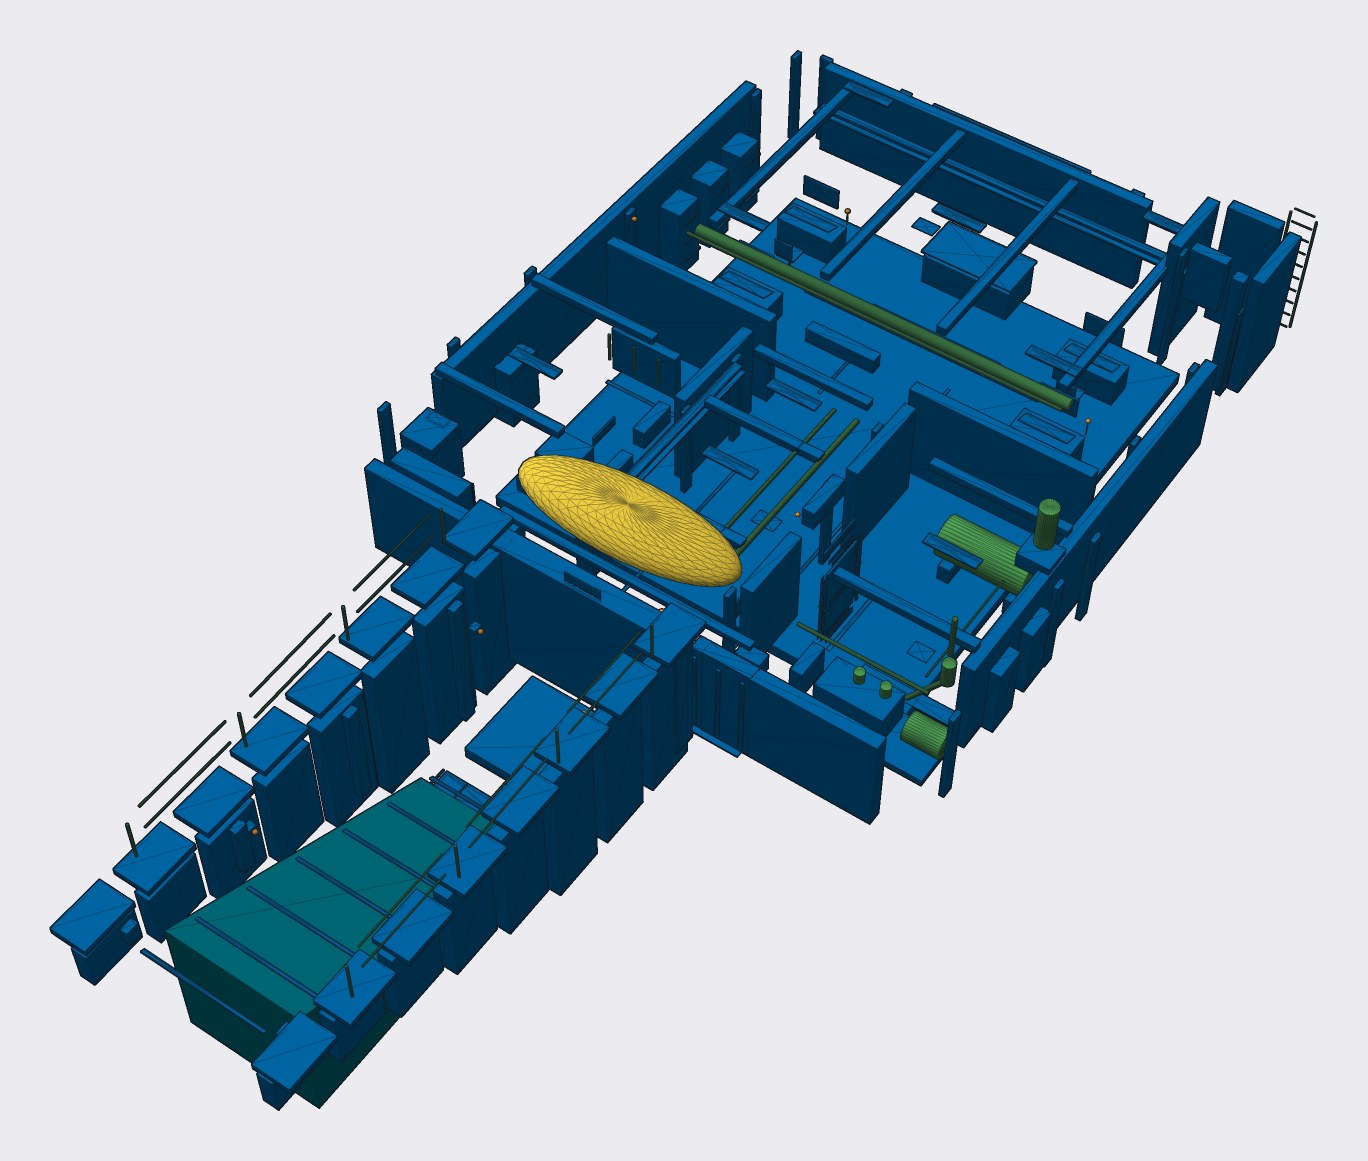
\includegraphics[width=6.60cm]{figures/img/shapes/command_bunker_cut_prims.jpg}};
\node[anchor=west,inner sep=1pt] (L0) at (6.85,5.25) {Command room};
\draw[black!70,line width=0.4pt] (L0.west) -- (4.54,4.24); \fill[black] (4.54,4.24) circle (0.6pt);
\node[anchor=west,inner sep=1pt] (L1) at (6.85,4.55) {Exit shaft};
\draw[black!70,line width=0.4pt] (L1.west) -- (6.11,4.23); \fill[black] (6.11,4.23) circle (0.6pt);
\node[anchor=west,inner sep=1pt] (L2) at (6.85,3.85) {Bunker shell};
\draw[black!70,line width=0.4pt] (L2.west) -- (4.10,3.81); \fill[black] (4.10,3.81) circle (0.6pt);
\node[anchor=west,inner sep=1pt] (L3) at (6.85,3.15) {Bunk room};
\draw[black!70,line width=0.4pt] (L3.west) -- (2.62,3.61); \fill[black] (2.62,3.61) circle (0.6pt);
\node[anchor=west,inner sep=1pt] (L4) at (6.85,2.45) {Tunnel};
\draw[black!70,line width=0.4pt] (L4.west) -- (3.52,3.13); \fill[black] (3.52,3.13) circle (0.6pt);
\node[anchor=west,inner sep=1pt] (L5) at (6.85,1.75) {Generator room};
\draw[black!70,line width=0.4pt] (L5.west) -- (4.50,2.72); \fill[black] (4.50,2.72) circle (0.6pt);
\node[anchor=west,inner sep=1pt] (L6) at (6.85,1.05) {Blast door assembly};
\draw[black!70,line width=0.4pt] (L6.west) -- (2.97,2.57); \fill[black] (2.97,2.57) circle (0.6pt);
\node[anchor=west,inner sep=1pt] (L7) at (6.85,0.35) {Entrance trench};
\draw[black!70,line width=0.4pt] (L7.west) -- (2.13,1.82); \fill[black] (2.13,1.82) circle (0.6pt);
\end{tikzpicture}\\[-0.3mm]{\fontsize{7.5}{9}\selectfont Full model} & {\fontsize{7.5}{9}\selectfont Made of primitives (pulled apart)}\end{tabular}
\\[0.8mm]{\fontsize{7}{8.5}\selectfont \primchipn{cuboid}{281}\quad \primchipn{wedge}{1}\quad \primchipn{sphere}{18}\quad \primchipn{hemisphere}{1}\quad \primchipn{capsule}{9}\quad \primchipn{cylinder}{80}\quad \textbf{total 390}\\pale: Camouflage net $\times$1 (37 parts)}\vspace{0.6mm}\end{minipage}}
\captionof{figure}{Command bunker. Cutaway: roof slabs, surface installations and camouflage net are left out in both panels (78 parts) so what they cover shows.}\label{fig:d-command_bunker}
\end{center}\vspace{-3mm}
\noindent\textbf{Command bunker.}\label{des:command_bunker} Underground command bunker with its surface installations. One instance, at the origin of the camp. Placement of the first: $T(0.00,\,0.00,\,0.00)\,R_y(0^\circ)\,S(1)$.
{\fontsize{7}{8.2}\selectfont\setlength{\tabcolsep}{2.6pt}\renewcommand{\arraystretch}{1.02}
\begin{longtable}{@{}>{\raggedright\arraybackslash}p{3.3cm}l>{\raggedright\arraybackslash}p{2.7cm}>{\raggedright\arraybackslash}p{4.2cm}>{\raggedright\arraybackslash}p{2.3cm}>{\raggedright\arraybackslash}p{2.4cm}@{}}
\toprule Part ($\times n$) & Shape & Size $S$ (cm) & Position $T$ (cm, design frame) & Rotation $R$ ($^\circ$) & Parent\\\midrule\endhead
\bottomrule\endfoot
\multicolumn{6}{@{}l}{\textit{Entrance trench}}\\[0.2mm]
Ramp floor & \primchip{wedge} & $320{\times}327{\times}700$ & $(0,\,-177,\,950)$ & $(0,\,180,\,0)$ & Entrance trench\\
Ramp grip strip $\times$7 & \primchip{cuboid} & $290{\times}3{\times}10$ & $(0,\,-305{+}46i,\,670{+}100i)$ & $(-25,\,0,\,0)$ & Entrance trench\\
Landing slab & \primchip{cuboid} & $320{\times}30{\times}235$ & $(0,\,-355,\,482)$ & -- & Entrance trench\\
Retaining wall W $\times$8 & \primchip{cuboid} & $35{\times}91.6..391{\times}124$ & $(-167,\,-182..-39,\,426{+}123i)$ & -- & Entrance trench\\
Coping slab W $\times$8 & \primchip{cuboid} & $85{\times}16{\times}126$ & $(-182,\,1..22,\,426{+}123i)$ & -- & Entrance trench\\
Counterfort rib $\times$8 & \primchip{cuboid} & $18{\times}39.3..361{\times}30$ & $(\pm 141,\,-164..-17,\,540..1260)$ & -- & Entrance trench\\
Retaining wall E $\times$8 & \primchip{cuboid} & $35{\times}91.6..391{\times}124$ & $(167,\,-182..-39,\,426{+}123i)$ & -- & Entrance trench\\
Coping slab E $\times$8 & \primchip{cuboid} & $85{\times}16{\times}126$ & $(182,\,1..22,\,426{+}123i)$ & -- & Entrance trench\\
Guard rail post $\times$8 & \primchip{cylinder} & $6{\times}6{\times}100$ & $(\pm 195,\,64..78,\,490{+}230i)$ & $(90,\,0,\,0)$ & Entrance trench\\
Guard rail $\times$12 & \primchip{cylinder} & $4{\times}4{\times}230$ & $(\pm 195,\,65..126,\,605{+}230i)$ & $(0{+}1i,\,0,\,0)$ & Entrance trench\\
Drain gutter & \primchip{cuboid} & $290{\times}2{\times}45$ & $(0,\,-339,\,650)$ & -- & Entrance trench\\
Drain frame & \primchip{cuboid} & $300{\times}4{\times}55$ & $(0,\,-338,\,650)$ & -- & Entrance trench\\
Drain grate bar $\times$6 & \primchip{cuboid} & $3{\times}4{\times}50$ & $(\pm(24{+}48i),\,-336,\,650)$ & -- & Entrance trench\\
Landing lamp housing & \primchip{cuboid} & $30{\times}12{\times}20$ & $(135,\,-80,\,560)$ & -- & Entrance trench\\
Landing floodlight & \primchip{sphere} & $18{\times}18{\times}6$ & $(115,\,-85,\,560)$ & $(90,\,0,\,0)$ & Entrance trench\\
Wall lamp housing $\times$4 & \primchip{cuboid} & $18{\times}12{\times}22$ & $(\pm 141,\,\{-120,-51,-45\},\,500{+}260i)$ & -- & Entrance trench\\
Wall lamp $\times$4 & \primchip{sphere} & $12{\times}12{\times}12$ & $(\pm 130,\,\{-122,-53,-47\},\,500{+}260i)$ & -- & Entrance trench\\
Portal head wall & \primchip{cuboid} & $480{\times}356{\times}55$ & $(0,\,-162,\,390)$ & -- & Entrance trench\\
Earth berm & \primchip{hemisphere} & $540{\times}50{\times}200$ & $(0,\,41,\,280)$ & -- & Entrance trench\\
Hazard jamb $\times$2 & \primchip{cuboid} & $20{\times}260{\times}5$ & $(\pm 140,\,-210,\,403)$ & -- & Entrance trench\\
Hazard header & \primchip{cuboid} & $300{\times}30{\times}5$ & $(0,\,-65,\,403)$ & -- & Entrance trench\\
Warning sign & \primchip{cuboid} & $90{\times}35{\times}3$ & $(0,\,-20,\,402)$ & -- & Entrance trench\\
\textit{Camouflage net} $\times$1 & \multicolumn{5}{@{}l}{\textit{nested design, drawn pale; its parts are counted in its own card (Figure~\ref{fig:d-camouflage_net})}}\\
\multicolumn{6}{@{}l}{\textit{Blast door assembly}}\\[0.2mm]
Leaf plate $\times$2 & \primchip{cuboid} & $145{\times}260{\times}35$ & $(\pm 222,\,-210,\,383)$ & -- & Door leaf\\
Leaf stiffener $\times$6 & \primchip{cuboid} & $10{\times}230{\times}5$ & $(\pm(177{+}45i),\,-210,\,402)$ & -- & Door leaf\\
Leaf edge stripe $\times$2 & \primchip{cuboid} & $12{\times}260{\times}4$ & $(\pm 156,\,-210,\,402)$ & -- & Door leaf\\
Locking bolt $\times$2 & \primchip{cylinder} & $12{\times}12{\times}20$ & $(\pm 167,\,-155,\,403)$ & -- & Door leaf\\
Door top rail & \primchip{cuboid} & $640{\times}14{\times}20$ & $(0,\,-87,\,355)$ & -- & Blast door assembly\\
Door floor rail & \primchip{cuboid} & $640{\times}4{\times}20$ & $(0,\,-338,\,383)$ & -- & Blast door assembly\\
Door drive motor $\times$2 & \primchip{cuboid} & $60{\times}45{\times}35$ & $(\pm 240,\,-135,\,347)$ & -- & Blast door assembly\\
Beacon base $\times$2 & \primchip{cylinder} & $22{\times}22{\times}10$ & $(\pm 110,\,-73,\,410)$ & $(90,\,0,\,0)$ & Blast door assembly\\
Beacon lamp $\times$4 & \primchip{sphere} & $16{\times}16{\times}16$ & $(\{-120,-100,110\},\,-54,\,400{+}10i)$ & -- & Beacon spinner\\
Beacon reflector $\times$2 & \primchip{cuboid} & $2{\times}14{\times}18$ & $(\pm 110,\,-54,\,410)$ & -- & Beacon spinner\\
Status lamp housing & \primchip{cuboid} & $18{\times}28{\times}8$ & $(-140,\,-170,\,404)$ & -- & Blast door assembly\\
Status lamp & \primchip{sphere} & $12{\times}12{\times}8$ & $(-140,\,-170,\,409)$ & -- & Blast door assembly\\
Front wall W & \primchip{cuboid} & $420{\times}260{\times}35$ & $(-340,\,-210,\,383)$ & -- & Blast door assembly\\
Front wall E & \primchip{cuboid} & $420{\times}260{\times}35$ & $(340,\,-210,\,383)$ & -- & Blast door assembly\\
\multicolumn{6}{@{}l}{\textit{Bunker shell}}\\[0.2mm]
Floor slab & \primchip{cuboid} & $1.1e+03{\times}30{\times}1.25e+03$ & $(0,\,-355,\,-225)$ & -- & Bunker shell\\
West wall & \primchip{cuboid} & $30{\times}260{\times}1.25e+03$ & $(-535,\,-210,\,-225)$ & -- & Bunker shell\\
East wall & \primchip{cuboid} & $30{\times}260{\times}1.06e+03$ & $(535,\,-210,\,-130)$ & -- & Bunker shell\\
South wall & \primchip{cuboid} & $910{\times}260{\times}30$ & $(-95,\,-210,\,-835)$ & -- & Bunker shell\\
Roof slab $\times$2 & \primchip{cuboid} & $910..1.1e+03{\times}35{\times}190..1.06e+03$ & $(\{-95,0\},\,-62,\,\{-755,-130\})$ & -- & Bunker shell\\
Tunnel wall W1 & \primchip{cuboid} & $30{\times}260{\times}270$ & $(-165,\,-210,\,-45)$ & -- & Bunker shell\\
Tunnel wall W2 & \primchip{cuboid} & $30{\times}260{\times}175$ & $(-165,\,-210,\,278)$ & -- & Bunker shell\\
Doorway lintel W & \primchip{cuboid} & $30{\times}50{\times}100$ & $(-165,\,-105,\,140)$ & -- & Bunker shell\\
Tunnel wall E1 & \primchip{cuboid} & $30{\times}260{\times}240$ & $(165,\,-210,\,-60)$ & -- & Bunker shell\\
Tunnel wall E2 & \primchip{cuboid} & $30{\times}260{\times}185$ & $(165,\,-210,\,272)$ & -- & Bunker shell\\
Doorway lintel E & \primchip{cuboid} & $30{\times}50{\times}120$ & $(165,\,-105,\,120)$ & -- & Bunker shell\\
Cross wall W & \primchip{cuboid} & $460{\times}260{\times}30$ & $(-320,\,-210,\,-195)$ & -- & Bunker shell\\
Cross wall E & \primchip{cuboid} & $460{\times}260{\times}30$ & $(320,\,-210,\,-195)$ & -- & Bunker shell\\
Doorway lintel CIC & \primchip{cuboid} & $180{\times}40{\times}30$ & $(0,\,-100,\,-195)$ & -- & Bunker shell\\
Shaft wall W & \primchip{cuboid} & $30{\times}348{\times}190$ & $(375,\,-166,\,-755)$ & -- & Bunker shell\\
Shaft wall E & \primchip{cuboid} & $30{\times}348{\times}190$ & $(535,\,-166,\,-755)$ & -- & Bunker shell\\
Shaft wall S & \primchip{cuboid} & $130{\times}348{\times}30$ & $(455,\,-166,\,-835)$ & -- & Bunker shell\\
Shaft wall N1 & \primchip{cuboid} & $10{\times}348{\times}30$ & $(395,\,-166,\,-675)$ & -- & Bunker shell\\
Shaft wall N2 & \primchip{cuboid} & $30{\times}348{\times}30$ & $(505,\,-166,\,-675)$ & -- & Bunker shell\\
Shaft door lintel & \primchip{cuboid} & $90{\times}148{\times}30$ & $(445,\,-66,\,-675)$ & -- & Bunker shell\\
\multicolumn{6}{@{}l}{\textit{Tunnel}}\\[0.2mm]
Fixture housing $\times$3 & \primchip{cuboid} & $130{\times}5{\times}30$ & $(0,\,-83,\,\{-90,100,300\})$ & -- & Tunnel\\
Tunnel tube & \primchip{cuboid} & $120{\times}5{\times}22$ & $(0,\,-87,\,300)$ & -- & Tunnel\\
Tunnel tube (light) $\times$2 & \primchip{cuboid} & $120{\times}5{\times}22$ & $(0,\,-87,\,\{-90,100\})$ & -- & Tunnel\\
Wall rib W $\times$3 & \primchip{cuboid} & $12{\times}260{\times}30$ & $(-144,\,-210,\,\{-130,20,310\})$ & -- & Tunnel\\
Wall rib E $\times$3 & \primchip{cuboid} & $12{\times}260{\times}30$ & $(144,\,-210,\,\{-130,20,310\})$ & -- & Tunnel\\
Ceiling beam $\times$3 & \primchip{cuboid} & $300{\times}20{\times}24$ & $(0,\,-90,\,\{-150,0,230\})$ & -- & Tunnel\\
Cable tray & \primchip{cuboid} & $40{\times}6{\times}520$ & $(-125,\,-109,\,90)$ & -- & Tunnel\\
Cable bundle & \primchip{cuboid} & $20{\times}10{\times}520$ & $(-125,\,-101,\,90)$ & -- & Tunnel\\
Water pipe & \primchip{cylinder} & $14{\times}14{\times}520$ & $(115,\,-95,\,90)$ & -- & Tunnel\\
Air duct pipe & \primchip{cylinder} & $10{\times}10{\times}520$ & $(70,\,-95,\,90)$ & -- & Tunnel\\
Floor line $\times$2 & \primchip{cuboid} & $8{\times}1.2{\times}500$ & $(\pm 112,\,-339,\,90)$ & -- & Tunnel\\
Door sill hazard & \primchip{cuboid} & $260{\times}1.2{\times}40$ & $(0,\,-339,\,340)$ & -- & Tunnel\\
Floor drain & \primchip{cuboid} & $60{\times}1.4{\times}40$ & $(0,\,-339,\,-20)$ & -- & Tunnel\\
Emergency exit sign & \primchip{cuboid} & $70{\times}22{\times}4$ & $(0,\,-111,\,342)$ & -- & Tunnel\\
Emergency lamp & \primchip{sphere} & $12{\times}10{\times}12$ & $(135,\,-125,\,100)$ & -- & Tunnel\\
Fire extinguisher & \primchip{cylinder} & $16{\times}16{\times}45$ & $(140,\,-270,\,260)$ & $(90,\,0,\,0)$ & Tunnel\\
Extinguisher bracket & \primchip{cuboid} & $10{\times}10{\times}20$ & $(145,\,-245,\,260)$ & -- & Tunnel\\
Sign board & \primchip{cuboid} & $4{\times}50{\times}100$ & $(148,\,-165,\,260)$ & -- & Tunnel\\
\multicolumn{6}{@{}l}{\textit{Command room}}\\[0.2mm]
Fixture housing $\times$5 & \primchip{cuboid} & $130{\times}5{\times}30$ & $(-320{+}320i,\,-83,\,\{-740,-540,-320\})$ & -- & Command room\\
CIC tube (light) $\times$5 & \primchip{cuboid} & $120{\times}5{\times}22$ & $(-320{+}320i,\,-87,\,\{-740,-540,-320\})$ & -- & Command room\\
Emergency lamp $\times$2 & \primchip{sphere} & $14{\times}12{\times}14$ & $(\pm 505,\,-125,\,\{-790,-240\})$ & -- & Command room\\
Wall rib W $\times$3 & \primchip{cuboid} & $12{\times}260{\times}30$ & $(-514,\,-210,\,\{-790,-650,-240\})$ & -- & Command room\\
Wall rib E $\times$3 & \primchip{cuboid} & $12{\times}260{\times}30$ & $(514,\,-210,\,\{-640,-470,-260\})$ & -- & Command room\\
Wall rib S $\times$3 & \primchip{cuboid} & $30{\times}260{\times}12$ & $(\{-460,-280,220\},\,-210,\,-814)$ & -- & Command room\\
Ceiling beam $\times$4 & \primchip{cuboid} & $24{\times}22{\times}610$ & $(\pm(120{+}240i),\,-91,\,-515)$ & -- & Command room\\
Cable tray & \primchip{cuboid} & $1.02e+03{\times}6{\times}40$ & $(0,\,-111,\,-680)$ & -- & Command room\\
Cable bundle & \primchip{cuboid} & $1e+03{\times}10{\times}20$ & $(0,\,-103,\,-680)$ & -- & Command room\\
Ventilation duct & \primchip{cylinder} & $30{\times}30{\times}1e+03$ & $(0,\,-110,\,-270)$ & $(0,\,90,\,0)$ & Command room\\
Pipe & \primchip{cylinder} & $9{\times}9{\times}1e+03$ & $(0,\,-92,\,-235)$ & $(0,\,90,\,0)$ & Command room\\
Floor line $\times$2 & \primchip{cuboid} & $8{\times}1.2{\times}190$ & $(\pm 95,\,-339,\,-315)$ & -- & Command room\\
Floor line ring N & \primchip{cuboid} & $360{\times}1.2{\times}8$ & $(0,\,-339,\,-496)$ & -- & Command room\\
Floor drain & \primchip{cuboid} & $60{\times}1.4{\times}40$ & $(-170,\,-339,\,-740)$ & -- & Command room\\
Cable cover & \primchip{cuboid} & $660{\times}3{\times}10$ & $(-10,\,-339,\,-455)$ & -- & Command room\\
Plotting table base & \primchip{cuboid} & $240{\times}85{\times}120$ & $(0,\,-298,\,-640)$ & -- & Command room\\
Plotting table top & \primchip{cuboid} & $250{\times}5{\times}130$ & $(0,\,-253,\,-640)$ & -- & Command room\\
Wall map frame & \primchip{cuboid} & $440{\times}140{\times}7$ & $(-50,\,-165,\,-816)$ & -- & Command room\\
Wall map screen & \primchip{cuboid} & $420{\times}126{\times}3$ & $(-50,\,-165,\,-811)$ & -- & Command room\\
Console desk $\times$4 & \primchip{cuboid} & $160{\times}75{\times}70$ & $(\{-320,300,320\},\,-303,\,\{-560,-540,-340\})$ & -- & Command room\\
Console keyboard screen $\times$4 & \primchip{cuboid} & $130{\times}4{\times}45$ & $(\{-320,300,320\},\,-262,\,\{-555,-535,-335\})$ & $(-18,\,0,\,0)$ & Command room\\
Console monitor $\times$4 & \primchip{cuboid} & $100{\times}55{\times}5$ & $(\{-320,300,320\},\,-218,\,\{-588,-568,-368\})$ & -- & Command room\\
Chair seat $\times$4 & \primchip{cuboid} & $50{\times}6{\times}50$ & $(\{-320,300,320\},\,-295,\,\{-485,-465,-265\})$ & -- & Command room\\
Chair back $\times$4 & \primchip{cuboid} & $50{\times}47{\times}5$ & $(\{-320,300,320\},\,-268,\,\{-461,-441,-241\})$ & -- & Command room\\
Chair post $\times$4 & \primchip{cylinder} & $7{\times}7{\times}42$ & $(\{-320,300,320\},\,-319,\,\{-485,-465,-265\})$ & $(90,\,0,\,0)$ & Command room\\
Task lamp arm $\times$2 & \primchip{cylinder} & $3{\times}3{\times}35$ & $(\{-255,385\},\,-247,\,\{-580,-360\})$ & $(90,\,0,\,0)$ & Command room\\
Task lamp $\times$2 & \primchip{sphere} & $13{\times}10{\times}13$ & $(\{-255,385\},\,-226,\,\{-580,-360\})$ & -- & Command room\\
Server rack $\times$3 & \primchip{cuboid} & $60{\times}200{\times}80$ & $(-490,\,-240,\,-560{+}100i)$ & -- & Command room\\
Rack LED row $\times$9 & \primchip{cuboid} & $3{\times}6{\times}60$ & $(-459,\,-277{+}45i,\,-560{+}100i)$ & -- & Command room\\
Notice board & \primchip{cuboid} & $10{\times}70{\times}80$ & $(515,\,-185,\,-320)$ & -- & Command room\\
Room sign & \primchip{cuboid} & $120{\times}25{\times}4$ & $(0,\,-112,\,-180)$ & -- & Command room\\
Fire extinguisher & \primchip{cylinder} & $16{\times}16{\times}45$ & $(-500,\,-300,\,-195)$ & $(90,\,0,\,0)$ & Command room\\
\multicolumn{6}{@{}l}{\textit{Bunk room}}\\[0.2mm]
Fixture housing & \primchip{cuboid} & $130{\times}5{\times}30$ & $(-350,\,-83,\,100)$ & -- & Bunk room\\
Bunk room tube (light) & \primchip{cuboid} & $120{\times}5{\times}22$ & $(-350,\,-87,\,100)$ & -- & Bunk room\\
Ceiling beam $\times$2 & \primchip{cuboid} & $340{\times}20{\times}24$ & $(-350,\,-90,\,\{-70,200\})$ & -- & Bunk room\\
Wall rib $\times$3 & \primchip{cuboid} & $12{\times}260{\times}30$ & $(-514,\,-210,\,\{-100,120,310\})$ & -- & Bunk room\\
Bunk frame $\times$2 & \primchip{cuboid} & $90{\times}170{\times}100$ & $(-470,\,-255,\,\{30,250\})$ & -- & Bunk room\\
Lower mattress $\times$2 & \primchip{cuboid} & $84{\times}17{\times}96$ & $(-470,\,-297,\,\{30,250\})$ & -- & Bunk room\\
Upper mattress $\times$2 & \primchip{cuboid} & $84{\times}17{\times}96$ & $(-470,\,-207,\,\{30,250\})$ & -- & Bunk room\\
Pillow $\times$2 & \primchip{cuboid} & $50{\times}8{\times}30$ & $(-475,\,-194,\,\{0,220\})$ & -- & Bunk room\\
Weapon rack & \primchip{cuboid} & $180{\times}130{\times}25$ & $(-310,\,-275,\,-167)$ & -- & Bunk room\\
Rifle $\times$3 & \primchip{cylinder} & $6{\times}6{\times}80$ & $(-380{+}55i,\,-265,\,-150)$ & $(-90,\,0,\,0)$ & Bunk room\\
Lockers & \primchip{cuboid} & $190{\times}190{\times}50$ & $(-395,\,-245,\,340)$ & -- & Bunk room\\
Locker door line $\times$3 & \primchip{cuboid} & $2{\times}170{\times}1$ & $(-450{+}63i,\,-245,\,314)$ & -- & Bunk room\\
Table & \primchip{cuboid} & $100{\times}75{\times}90$ & $(-300,\,-303,\,95)$ & -- & Bunk room\\
Bench & \primchip{cuboid} & $120{\times}42{\times}30$ & $(-300,\,-319,\,165)$ & -- & Bunk room\\
Room sign & \primchip{cuboid} & $4{\times}25{\times}80$ & $(-176,\,-112,\,140)$ & -- & Bunk room\\
Fire extinguisher & \primchip{cylinder} & $16{\times}16{\times}45$ & $(-200,\,-300,\,340)$ & $(90,\,0,\,0)$ & Bunk room\\
Floor line & \primchip{cuboid} & $200{\times}1.2{\times}10$ & $(-300,\,-339,\,-135)$ & -- & Bunk room\\
\multicolumn{6}{@{}l}{\textit{Generator room}}\\[0.2mm]
Fixture housing & \primchip{cuboid} & $130{\times}5{\times}30$ & $(350,\,-83,\,60)$ & -- & Generator room\\
Plant room tube (light) & \primchip{cuboid} & $120{\times}5{\times}22$ & $(350,\,-87,\,60)$ & -- & Generator room\\
Ceiling beam $\times$2 & \primchip{cuboid} & $340{\times}20{\times}24$ & $(350,\,-90,\,\{-90,200\})$ & -- & Generator room\\
Wall rib $\times$3 & \primchip{cuboid} & $12{\times}260{\times}30$ & $(514,\,-210,\,\{-120,0,320\})$ & -- & Generator room\\
Generator skid & \primchip{cuboid} & $270{\times}18{\times}130$ & $(365,\,-331,\,265)$ & -- & Generator room\\
Generator engine block & \primchip{cuboid} & $170{\times}82{\times}90$ & $(315,\,-281,\,265)$ & -- & Generator room\\
Generator alternator & \primchip{cylinder} & $70{\times}70{\times}90$ & $(445,\,-275,\,265)$ & $(0,\,90,\,0)$ & Generator room\\
Generator radiator & \primchip{cuboid} & $30{\times}80{\times}90$ & $(215,\,-275,\,265)$ & -- & Generator room\\
Generator cylinder head $\times$2 & \primchip{cylinder} & $25{\times}25{\times}30$ & $(\{310,360\},\,-225,\,260)$ & $(90,\,0,\,0)$ & Generator room\\
Exhaust pipe & \primchip{cylinder} & $12{\times}12{\times}105$ & $(423,\,-190,\,250)$ & $(-50,\,107,\,0)$ & Generator room\\
Exhaust silencer & \primchip{cylinder} & $30{\times}30{\times}60$ & $(455,\,-130,\,240)$ & $(90,\,0,\,0)$ & Generator room\\
Exhaust riser & \primchip{cylinder} & $12{\times}12{\times}115$ & $(455,\,-43,\,240)$ & $(90,\,0,\,0)$ & Generator room\\
Control cabinet & \primchip{cuboid} & $50{\times}190{\times}80$ & $(495,\,-245,\,140)$ & -- & Generator room\\
Switchgear cabinet & \primchip{cuboid} & $50{\times}190{\times}80$ & $(495,\,-245,\,40)$ & -- & Generator room\\
Cabinet display & \primchip{cuboid} & $4{\times}30{\times}60$ & $(468,\,-195,\,140)$ & -- & Generator room\\
Fuel tank & \primchip{cylinder} & $100{\times}100{\times}220$ & $(340,\,-255,\,-100)$ & $(0,\,90,\,0)$ & Generator room\\
Tank saddle $\times$2 & \primchip{cuboid} & $30{\times}45{\times}80$ & $(\{275,405\},\,-318,\,-100)$ & -- & Generator room\\
Fuel line & \primchip{cylinder} & $5{\times}5{\times}320$ & $(390,\,-250,\,60)$ & -- & Generator room\\
Ventilation unit & \primchip{cuboid} & $80{\times}40{\times}70$ & $(460,\,-115,\,-35)$ & -- & Generator room\\
Ventilation riser & \primchip{cylinder} & $45{\times}45{\times}110$ & $(460,\,-40,\,-40)$ & $(90,\,0,\,0)$ & Generator room\\
Floor line & \primchip{cuboid} & $10{\times}1.2{\times}200$ & $(195,\,-339,\,90)$ & -- & Generator room\\
Floor drain & \primchip{cuboid} & $50{\times}1.4{\times}40$ & $(325,\,-339,\,80)$ & -- & Generator room\\
Hazard marking & \primchip{cuboid} & $270{\times}1.2{\times}40$ & $(365,\,-339,\,170)$ & -- & Generator room\\
Room sign & \primchip{cuboid} & $4{\times}25{\times}120$ & $(176,\,-112,\,120)$ & -- & Generator room\\
Door leaf & \primchip{cuboid} & $5{\times}206{\times}117$ & $(176,\,-235,\,120)$ & -- & GENERATOR ROOM DOOR hinge\\
Hinge stile $\times$2 & \primchip{cuboid} & $1.2{\times}206{\times}11$ & $(\{173,180\},\,-235,\,68)$ & -- & GENERATOR ROOM DOOR hinge\\
Lock stile $\times$2 & \primchip{cuboid} & $1.2{\times}206{\times}11$ & $(\{173,180\},\,-235,\,174)$ & -- & GENERATOR ROOM DOOR hinge\\
Top rail $\times$2 & \primchip{cuboid} & $1.2{\times}12{\times}95$ & $(\{173,180\},\,-138,\,120)$ & -- & GENERATOR ROOM DOOR hinge\\
Lock rail $\times$2 & \primchip{cuboid} & $1.2{\times}14{\times}95$ & $(\{173,180\},\,-238,\,120)$ & -- & GENERATOR ROOM DOOR hinge\\
Bottom rail $\times$2 & \primchip{cuboid} & $1.2{\times}22{\times}95$ & $(\{173,180\},\,-327,\,120)$ & -- & GENERATOR ROOM DOOR hinge\\
Kick plate $\times$2 & \primchip{cuboid} & $0.4{\times}20{\times}111$ & $(\{173,180\},\,-327,\,120)$ & -- & GENERATOR ROOM DOOR hinge\\
Handle rose $\times$2 & \primchip{cylinder} & $6.5{\times}6.5{\times}1.2$ & $(\{172,181\},\,-238,\,171)$ & $(0,\,90,\,0)$ & GENERATOR ROOM DOOR hinge\\
Handle spindle $\times$2 & \primchip{cylinder} & $2{\times}2{\times}5$ & $(\{169,183\},\,-238,\,171)$ & $(0,\,90,\,0)$ & GENERATOR ROOM DOOR hinge\\
Handle lever $\times$2 & \primchip{cuboid} & $2.2{\times}2.4{\times}13$ & $(\{167,186\},\,-238,\,166)$ & -- & GENERATOR ROOM DOOR hinge\\
Key cylinder $\times$2 & \primchip{cylinder} & $3{\times}3{\times}1.6$ & $(\{172,181\},\,-251,\,171)$ & $(0,\,90,\,0)$ & GENERATOR ROOM DOOR hinge\\
Hinge knuckle $\times$3 & \primchip{cylinder} & $2.6{\times}2.6{\times}11$ & $(179,\,\{-316,-225,-154\},\,61)$ & $(90,\,0,\,0)$ & GENERATOR ROOM DOOR hinge\\
Hinge leaf $\times$3 & \primchip{cuboid} & $0.4{\times}10{\times}6$ & $(179,\,\{-316,-225,-154\},\,64)$ & -- & GENERATOR ROOM DOOR hinge\\
Fire extinguisher & \primchip{cylinder} & $16{\times}16{\times}45$ & $(210,\,-300,\,340)$ & $(90,\,0,\,0)$ & Generator room\\
Ceiling pipe & \primchip{cylinder} & $9{\times}9{\times}310$ & $(345,\,-92,\,320)$ & $(0,\,90,\,0)$ & Generator room\\
\multicolumn{6}{@{}l}{\textit{Exit shaft}}\\[0.2mm]
Shaft lamp & \primchip{sphere} & $14{\times}14{\times}14$ & $(400,\,-110,\,-760)$ & -- & Exit shaft\\
Ladder rail $\times$2 & \primchip{cylinder} & $5{\times}5{\times}333$ & $(\{430,480\},\,-173,\,-810)$ & $(90,\,0,\,0)$ & Exit shaft\\
Ladder rung $\times$10 & \primchip{cylinder} & $3{\times}3{\times}50$ & $(455,\,-305{+}30i,\,-810)$ & $(0,\,90,\,0)$ & Exit shaft\\
Exit sign & \primchip{cuboid} & $50{\times}20{\times}4$ & $(455,\,-100,\,-693)$ & -- & Exit shaft\\
\multicolumn{6}{@{}l}{\textit{Surface installations}}\\[0.2mm]
Vent stack A (exhaust) & \primchip{cuboid} & $75{\times}120{\times}75$ & $(455,\,60,\,240)$ & -- & Surface installations\\
Stack louvre $\times$4 & \primchip{cuboid} & $78{\times}5{\times}78$ & $(\{455,460\},\,25..60,\,\{-40,240\})$ & -- & Surface installations\\
Stack rain cap rim $\times$2 & \primchip{cuboid} & $85{\times}6{\times}85$ & $(\{455,460\},\,\{113,123\},\,\{-40,240\})$ & -- & Surface installations\\
Fan disc $\times$2 & \primchip{cylinder} & $60{\times}60{\times}3$ & $(\{455,460\},\,\{120,130\},\,\{-40,240\})$ & -- & Fan\\
Fan blade $\times$4 & \primchip{cuboid} & $58{\times}7{\times}2$ & $(\{455,460\},\,\{117,127\},\,\{-40,240\})$ & $(0,\,0,\,\{20,110\})$ & Fan\\
Vent stack B (intake) & \primchip{cuboid} & $75{\times}120{\times}75$ & $(460,\,50,\,-40)$ & -- & Surface installations\\
Beacon mast base & \primchip{cuboid} & $40{\times}30{\times}40$ & $(-360,\,10,\,160)$ & -- & Surface installations\\
Beacon mast & \primchip{cylinder} & $9{\times}9{\times}400$ & $(-360,\,210,\,160)$ & $(90,\,0,\,0)$ & Surface installations\\
Beacon housing & \primchip{cylinder} & $22{\times}22{\times}10$ & $(-360,\,415,\,160)$ & $(90,\,0,\,0)$ & Surface installations\\
Beacon bulb & \primchip{sphere} & $20{\times}20{\times}20$ & $(-360,\,430,\,160)$ & -- & Surface installations\\
Periscope tube & \primchip{cylinder} & $16{\times}16{\times}90$ & $(80,\,42,\,-460)$ & $(90,\,0,\,0)$ & Surface installations\\
Periscope head & \primchip{cuboid} & $30{\times}18{\times}30$ & $(80,\,94,\,-460)$ & -- & Surface installations\\
Periscope lens & \primchip{cylinder} & $10{\times}10{\times}4$ & $(80,\,94,\,-444)$ & -- & Surface installations\\
Antenna base & \primchip{cuboid} & $40{\times}25{\times}40$ & $(-400,\,13,\,-600)$ & -- & Surface installations\\
Antenna mast & \primchip{cylinder} & $5{\times}5{\times}320$ & $(-400,\,178,\,-600)$ & $(90,\,0,\,0)$ & Surface installations\\
Antenna dish & \primchip{sphere} & $70{\times}70{\times}12$ & $(-400,\,268,\,-590)$ & -- & Surface installations\\
Hatch collar & \primchip{cuboid} & $180{\times}30{\times}180$ & $(455,\,-7,\,-755)$ & -- & Surface installations\\
Hatch lid & \primchip{cuboid} & $145{\times}10{\times}145$ & $(455,\,13,\,-755)$ & -- & Surface installations\\
Hatch wheel & \primchip{cylinder} & $40{\times}40{\times}4$ & $(455,\,22,\,-755)$ & $(90,\,0,\,0)$ & Surface installations\\
Hatch wheel spoke $\times$2 & \primchip{cuboid} & $5..44{\times}5{\times}5..44$ & $(455,\,26,\,-755)$ & -- & Surface installations\\
Hatch hinge & \primchip{cuboid} & $100{\times}6{\times}10$ & $(455,\,19,\,-830)$ & -- & Surface installations\\
Sandbag $\times$9 & \primchip{capsule} & $24{\times}18{\times}50$ & $(336..603,\,-19..-13,\,-893..-681)$ & $(0,\,-302{+}22i,\,0)$ & Surface installations\\
\end{longtable}}
\bunkerextras

\needspace{10.6cm}
\begin{center}
\fcolorbox{black!30}{white}{\begin{minipage}{0.975\linewidth}\centering\vspace{0.6mm}
\begin{tabular}{@{}c@{\hspace{3mm}}c@{}}\img{figures/img/shapes/barracks_hall_cut_model.jpg}{5.18cm} & \begin{tikzpicture}[font=\fontsize{7}{8}\selectfont]
\node[inner sep=0,anchor=south west] at (0,0) {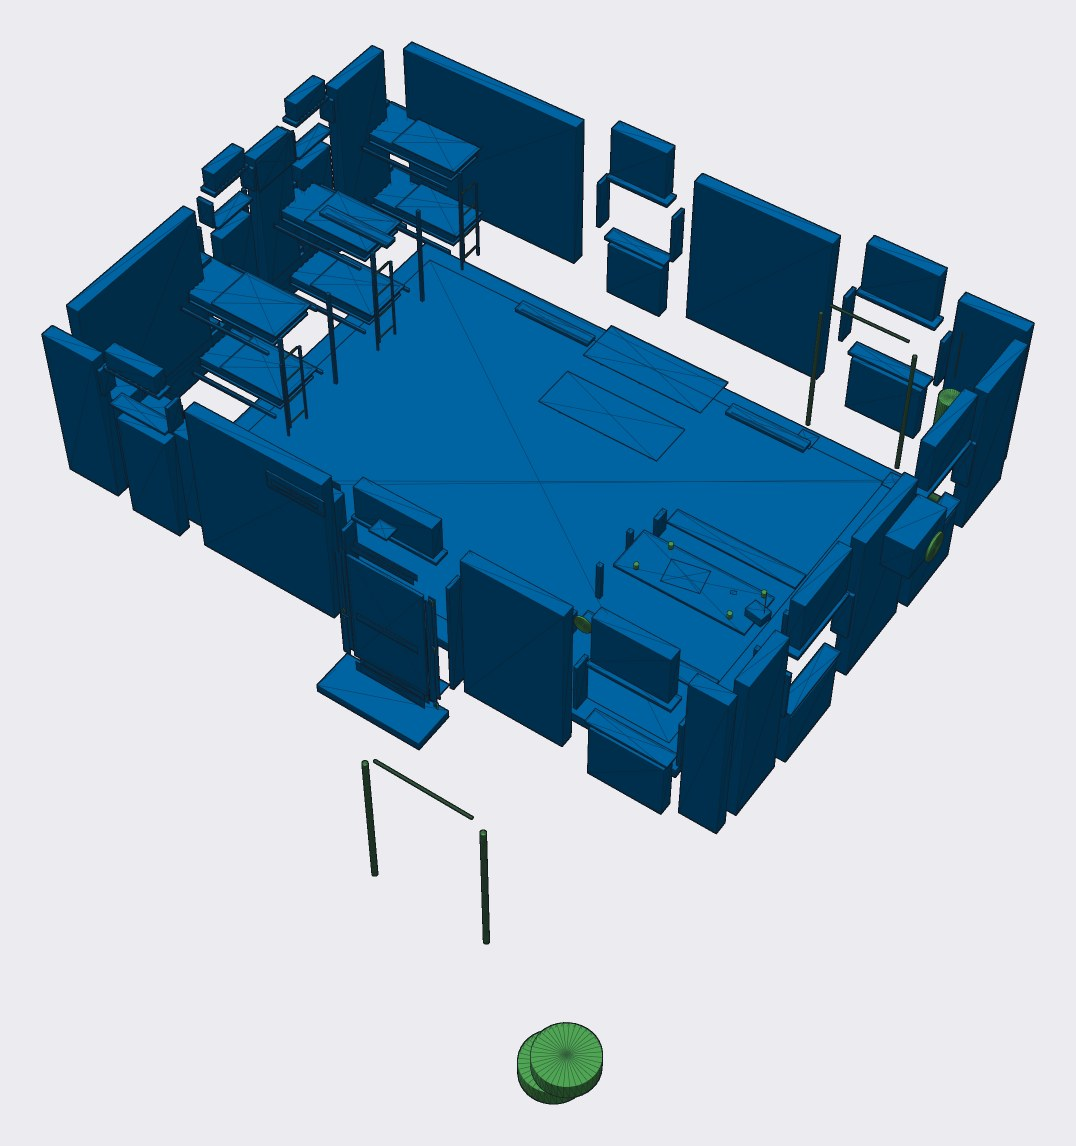
\includegraphics[width=5.26cm]{figures/img/shapes/barracks_hall_cut_prims.jpg}};
\node[anchor=west,inner sep=1pt] (L0) at (5.51,4.20) {Bunk bed};
\draw[black!70,line width=0.4pt] (L0.west) -- (2.05,4.77); \fill[black] (2.05,4.77) circle (0.6pt);
\draw[black!70,line width=0.4pt] (L0.west) -- (1.63,4.39); \fill[black] (1.63,4.39) circle (0.6pt);
\draw[black!70,line width=0.4pt] (L0.west) -- (1.19,3.99); \fill[black] (1.19,3.99) circle (0.6pt);
\node[anchor=west,inner sep=1pt] (L1) at (5.51,1.40) {BARRACKS DOOR hinge};
\draw[black!70,line width=0.4pt] (L1.west) -- (1.90,2.54); \fill[black] (1.90,2.54) circle (0.6pt);
\end{tikzpicture}\\[-0.3mm]{\fontsize{7.5}{9}\selectfont Full model} & {\fontsize{7.5}{9}\selectfont Made of primitives (pulled apart)}\end{tabular}
\\[0.8mm]{\fontsize{7}{8.5}\selectfont \primchipn{cuboid}{225}\quad \primchipn{sphere}{2}\quad \primchipn{cylinder}{50}\quad \textbf{total 277}}\vspace{0.6mm}\end{minipage}}
\captionof{figure}{Barracks hall. Cutaway: roof sheet, ridge cap, ceiling and gable are left out in both panels (14 parts) so what they cover shows.}\label{fig:d-barracks_hall}
\end{center}\vspace{-3mm}
\noindent\textbf{Barracks hall.}\label{des:barracks_hall} Enterable prefab barracks: bunks, lockers, mess table, gym corner. One instance, at the origin of the camp. Placement of the first: $T(0.00,\,0.00,\,0.00)\,R_y(0^\circ)\,S(1)$.
{\fontsize{7}{8.2}\selectfont\setlength{\tabcolsep}{2.6pt}\renewcommand{\arraystretch}{1.02}
\begin{longtable}{@{}>{\raggedright\arraybackslash}p{3.3cm}l>{\raggedright\arraybackslash}p{2.7cm}>{\raggedright\arraybackslash}p{4.2cm}>{\raggedright\arraybackslash}p{2.3cm}>{\raggedright\arraybackslash}p{2.4cm}@{}}
\toprule Part ($\times n$) & Shape & Size $S$ (cm) & Position $T$ (cm, design frame) & Rotation $R$ ($^\circ$) & Parent\\\midrule\endhead
\bottomrule\endfoot
\multicolumn{6}{@{}l}{\textit{Barracks hall}}\\[0.2mm]
Floor slab & \primchip{cuboid} & $920{\times}17{\times}660$ & $(2310,\,-28,\,-1180)$ & -- & root\\
Plank floor & \primchip{cuboid} & $856{\times}1.2{\times}596$ & $(2310,\,-19,\,-1180)$ & -- & root\\
North wall $\times$10 & \primchip{cuboid} & $60..240{\times}2..282{\times}22$ & $(1908..2730,\,-19..244,\,-871)$ & -- & root\\
Opening frame $\times$35 & \primchip{cuboid} & $6..142{\times}5..220{\times}6..132$ & $(1871..2749,\,79..230,\,-1489..-871)$ & -- & root\\
South wall $\times$7 & \primchip{cuboid} & $100..330{\times}90..282{\times}22$ & $(2025..2705,\,\{31,121,217\},\,-1489)$ & -- & root\\
East wall $\times$7 & \primchip{cuboid} & $22{\times}90..282{\times}98..140$ & $(2749,\,\{31,121,217\},\,-1419..-931)$ & -- & root\\
West wall $\times$7 & \primchip{cuboid} & $22{\times}35..282{\times}70..258$ & $(1871,\,\{81,121,244\},\,-1419..-1011)$ & -- & root\\
Wall lining $\times$2 & \primchip{cuboid} & $1.2{\times}60{\times}596$ & $(\{1883,2737\},\,12,\,-1180)$ & -- & root\\
Ceiling & \primchip{cuboid} & $856{\times}8{\times}596$ & $(2310,\,256,\,-1180)$ & -- & root\\
Roof sheet $\times$2 & \primchip{cuboid} & $960{\times}5{\times}372$ & $(2310,\,311,\,\{-1357,-1003\})$ & $(\pm 17,\,0,\,0)$ & root\\
Ridge cap & \primchip{cuboid} & $960{\times}8{\times}24$ & $(2310,\,366,\,-1180)$ & -- & root\\
Gable $\times$10 & \primchip{cuboid} & $22{\times}20{\times}64..576$ & $(\{1871,2749\},\,272{+}20i,\,-1180)$ & -- & root\\
Door step & \primchip{cuboid} & $180{\times}14{\times}70$ & $(2350,\,-27,\,-825)$ & -- & root\\
Door lamp hood & \primchip{cuboid} & $30{\times}4{\times}24$ & $(2350,\,237,\,-846)$ & -- & root\\
Hall door lamp & \primchip{sphere} & $13{\times}8{\times}13$ & $(2350,\,230,\,-846)$ & -- & root\\
Sign board & \primchip{cuboid} & $100{\times}32{\times}3$ & $(2225,\,202,\,-857)$ & -- & root\\
Sign letters & \primchip{cuboid} & $80{\times}10{\times}1$ & $(2225,\,202,\,-855)$ & -- & root\\
Hall AC unit & \primchip{cuboid} & $45{\times}60{\times}90$ & $(2783,\,202,\,-1175)$ & -- & root\\
Hall AC fan & \primchip{cylinder} & $45{\times}45{\times}4$ & $(2807,\,202,\,-1175)$ & $(0,\,90,\,0)$ & root\\
Locker $\times$6 & \primchip{cuboid} & $54.7{\times}185{\times}48$ & $(1928{+}57i,\,75,\,-906)$ & -- & root\\
Locker vents $\times$6 & \primchip{cuboid} & $28.3{\times}12{\times}1$ & $(1928{+}57i,\,142,\,-931)$ & -- & root\\
Locker handle $\times$6 & \primchip{cuboid} & $3{\times}12{\times}3$ & $(1949{+}56i,\,87,\,-932)$ & -- & root\\
Name tag $\times$6 & \primchip{cuboid} & $14{\times}5{\times}0.5$ & $(1928{+}57i,\,122,\,-930)$ & -- & root\\
Duffel bag & \primchip{cylinder} & $32{\times}32{\times}70$ & $(1960,\,182,\,-907)$ & $(0,\,90,\,0)$ & root\\
Rifle rack & \primchip{cuboid} & $80{\times}12{\times}25$ & $(2485,\,-12,\,-895)$ & -- & root\\
Racked rifle $\times$3 & \primchip{cuboid} & $5{\times}95{\times}6$ & $(2460{+}25i,\,42,\,-896)$ & $(-8,\,0,\,0)$ & root\\
Notice board & \primchip{cuboid} & $90{\times}60{\times}2$ & $(2485,\,147,\,-883)$ & -- & root\\
Notice $\times$4 & \primchip{cuboid} & $18{\times}24{\times}0.4$ & $(2455{+}20i,\,\{150,156\},\,-884)$ & $(0,\,0,\,\pm(2{+}4i))$ & root\\
Mess table top & \primchip{cuboid} & $220{\times}5{\times}80$ & $(2570,\,56,\,-1100)$ & -- & root\\
Table leg $\times$4 & \primchip{cuboid} & $8{\times}72{\times}8$ & $(\{2468,2672\},\,18,\,\{-1130,-1070\})$ & -- & root\\
Bench seat $\times$2 & \primchip{cuboid} & $220{\times}4{\times}30$ & $(2570,\,26,\,\{-1190,-1010\})$ & -- & root\\
Bench leg $\times$4 & \primchip{cuboid} & $8{\times}42{\times}24$ & $(\{2470,2670\},\,3,\,\{-1190,-1010\})$ & -- & root\\
Mug $\times$4 & \primchip{cylinder} & $8{\times}8{\times}10$ & $(2510..2645,\,64,\,\{-1124,-1078\})$ & $(90,\,0,\,0)$ & root\\
Map sheet & \primchip{cuboid} & $60{\times}0.4{\times}45$ & $(2560,\,59,\,-1100)$ & $(0,\,12,\,0)$ & root\\
Field radio & \primchip{cuboid} & $30{\times}16{\times}22$ & $(2655,\,67,\,-1095)$ & $(0,\,-10,\,0)$ & root\\
Radio antenna & \primchip{cylinder} & $1{\times}1{\times}45$ & $(2665,\,97,\,-1090)$ & $(90,\,0,\,0)$ & root\\
Playing cards & \primchip{cuboid} & $9{\times}1.2{\times}6$ & $(2615,\,60,\,-1110)$ & $(0,\,25,\,0)$ & root\\
Pull-up post $\times$2 & \primchip{cylinder} & $6{\times}6{\times}235$ & $(\{2530,2650\},\,99,\,-1415)$ & $(90,\,0,\,0)$ & root\\
Post foot $\times$2 & \primchip{cuboid} & $30{\times}2{\times}30$ & $(\{2530,2650\},\,-17,\,-1415)$ & -- & root\\
Pull-up bar & \primchip{cylinder} & $3.5{\times}3.5{\times}130$ & $(2590,\,207,\,-1415)$ & $(0,\,90,\,0)$ & root\\
Exercise mat $\times$2 & \primchip{cuboid} & $220{\times}2{\times}80$ & $(2320,\,-17,\,\{-1410,-1315\})$ & -- & root\\
Dumbbell rack & \primchip{cuboid} & $36{\times}75{\times}100$ & $(2718,\,19,\,-1325)$ & -- & root\\
Dumbbell $\times$8 & \primchip{cylinder} & $11..17{\times}11..17{\times}30$ & $(2718,\,\{24,54\},\,-1360{+}25i)$ & $(0,\,90,\,0)$ & root\\
Punching bag & \primchip{cylinder} & $36{\times}36{\times}100$ & $(2693,\,97,\,-1433)$ & $(90,\,0,\,0)$ & root\\
Bag chain & \primchip{cylinder} & $2{\times}2{\times}90$ & $(2693,\,202,\,-1433)$ & $(90,\,0,\,0)$ & root\\
Kettlebell & \primchip{sphere} & $22{\times}22{\times}22$ & $(2703,\,-7,\,-1245)$ & -- & root\\
Map board & \primchip{cuboid} & $2{\times}80{\times}120$ & $(2737,\,137,\,-1175)$ & -- & root\\
Map pins & \primchip{cuboid} & $1{\times}40{\times}60$ & $(2736,\,142,\,-1170)$ & -- & root\\
Wall flag & \primchip{cuboid} & $2{\times}60{\times}90$ & $(1883,\,207,\,-1250)$ & -- & root\\
Wall clock & \primchip{cylinder} & $28{\times}28{\times}3$ & $(2570,\,202,\,-884)$ & -- & root\\
Light fitting $\times$3 & \primchip{cuboid} & $124{\times}6{\times}20$ & $(2060{+}270i,\,249,\,-1180)$ & -- & root\\
Ceiling tube (light) $\times$3 & \primchip{cylinder} & $5{\times}5{\times}115$ & $(2060{+}270i,\,244,\,-1180)$ & $(0,\,90,\,0)$ & root\\
PT frame post $\times$2 & \primchip{cylinder} & $8{\times}8{\times}250$ & $(\{2490,2630\},\,95,\,-630)$ & $(90,\,0,\,0)$ & root\\
PT bar & \primchip{cylinder} & $4{\times}4{\times}150$ & $(2560,\,205,\,-630)$ & $(0,\,90,\,0)$ & root\\
PT tyre $\times$2 & \primchip{cylinder} & $90{\times}90{\times}28$ & $(\{2760,2775\},\,\{-16,12\},\,-560)$ & $(90,\,0,\,0)$ & root\\
\multicolumn{6}{@{}l}{\textit{BARRACKS DOOR hinge}}\\[0.2mm]
Door leaf & \primchip{cuboid} & $5{\times}218{\times}128$ & $(2350,\,92,\,-864)$ & -- & BARRACKS DOOR hinge\\
Hinge stile $\times$2 & \primchip{cuboid} & $1.2{\times}218{\times}11$ & $(2408,\,92,\,\{-867,-860\})$ & -- & BARRACKS DOOR hinge\\
Lock stile $\times$2 & \primchip{cuboid} & $1.2{\times}218{\times}11$ & $(2291,\,92,\,\{-867,-860\})$ & -- & BARRACKS DOOR hinge\\
Top rail $\times$2 & \primchip{cuboid} & $1.2{\times}12{\times}106$ & $(2350,\,195,\,\{-867,-860\})$ & -- & BARRACKS DOOR hinge\\
Lock rail $\times$2 & \primchip{cuboid} & $1.2{\times}14{\times}106$ & $(2350,\,83,\,\{-867,-860\})$ & -- & BARRACKS DOOR hinge\\
Bottom rail $\times$2 & \primchip{cuboid} & $1.2{\times}22{\times}106$ & $(2350,\,-6,\,\{-867,-860\})$ & -- & BARRACKS DOOR hinge\\
Kick plate $\times$2 & \primchip{cuboid} & $0.4{\times}20{\times}122$ & $(2350,\,-6,\,\{-867,-860\})$ & -- & BARRACKS DOOR hinge\\
Handle rose $\times$2 & \primchip{cylinder} & $6.5{\times}6.5{\times}1.2$ & $(2293,\,83,\,\{-868,-859\})$ & $(0,\,90,\,0)$ & BARRACKS DOOR hinge\\
Handle spindle $\times$2 & \primchip{cylinder} & $2{\times}2{\times}5$ & $(2293,\,83,\,\{-870,-857\})$ & $(0,\,90,\,0)$ & BARRACKS DOOR hinge\\
Handle lever $\times$2 & \primchip{cuboid} & $2.2{\times}2.4{\times}13$ & $(2299,\,83,\,\{-873,-854\})$ & -- & BARRACKS DOOR hinge\\
Key cylinder $\times$2 & \primchip{cylinder} & $3{\times}3{\times}1.6$ & $(2293,\,70,\,\{-868,-859\})$ & $(0,\,90,\,0)$ & BARRACKS DOOR hinge\\
Hinge knuckle $\times$3 & \primchip{cylinder} & $2.6{\times}2.6{\times}11$ & $(2415,\,\{5,102,179\},\,-859)$ & $(90,\,0,\,0)$ & BARRACKS DOOR hinge\\
Hinge leaf $\times$3 & \primchip{cuboid} & $2.5{\times}10{\times}6.2$ & $(2412,\,\{5,102,179\},\,-860)$ & -- & BARRACKS DOOR hinge\\
\multicolumn{6}{@{}l}{\textit{Bunk bed}}\\[0.2mm]
Bunk post $\times$12 & \primchip{cuboid} & $5{\times}192{\times}5$ & $(\{1888,2082\},\,78,\,-1445..-1055)$ & -- & Bunk bed\\
Bunk rail $\times$12 & \primchip{cuboid} & $200{\times}6{\times}4$ & $(1985,\,\{10,115\},\,-1445..-1055)$ & -- & Bunk bed\\
Bunk springs $\times$6 & \primchip{cuboid} & $192{\times}3{\times}83$ & $(1985,\,\{11,116\},\,-1400{+}150i)$ & -- & Bunk bed\\
Mattress $\times$6 & \primchip{cuboid} & $190{\times}14{\times}81$ & $(1985,\,\{20,125\},\,-1400{+}150i)$ & -- & Bunk bed\\
Pillow $\times$6 & \primchip{cuboid} & $34{\times}9{\times}62$ & $(1910,\,\{31,136\},\,-1400{+}150i)$ & -- & Bunk bed\\
Blanket $\times$6 & \primchip{cuboid} & $125{\times}3.5{\times}85$ & $(2017,\,\{29,134\},\,-1400{+}150i)$ & -- & Bunk bed\\
Head rail $\times$6 & \primchip{cuboid} & $4{\times}30{\times}89$ & $(1887,\,\{37,142\},\,-1400{+}150i)$ & -- & Bunk bed\\
Ladder rail $\times$6 & \primchip{cuboid} & $3{\times}155{\times}3$ & $(2087,\,60,\,-1381..-1047)$ & -- & Bunk bed\\
Ladder rung $\times$12 & \primchip{cylinder} & $2.5{\times}2.5{\times}34$ & $(2087,\,17{+}35i,\,-1364{+}150i)$ & -- & Bunk bed\\
\end{longtable}}

\needspace{10.6cm}
\begin{center}
\fcolorbox{black!30}{white}{\begin{minipage}{0.975\linewidth}\centering\vspace{0.6mm}
\begin{tabular}{@{}c@{\hspace{3mm}}c@{}}\img{figures/img/shapes/air_defence_radar_model.jpg}{4.72cm} & \begin{tikzpicture}[font=\fontsize{7}{8}\selectfont]
\node[inner sep=0,anchor=south west] at (0,0) {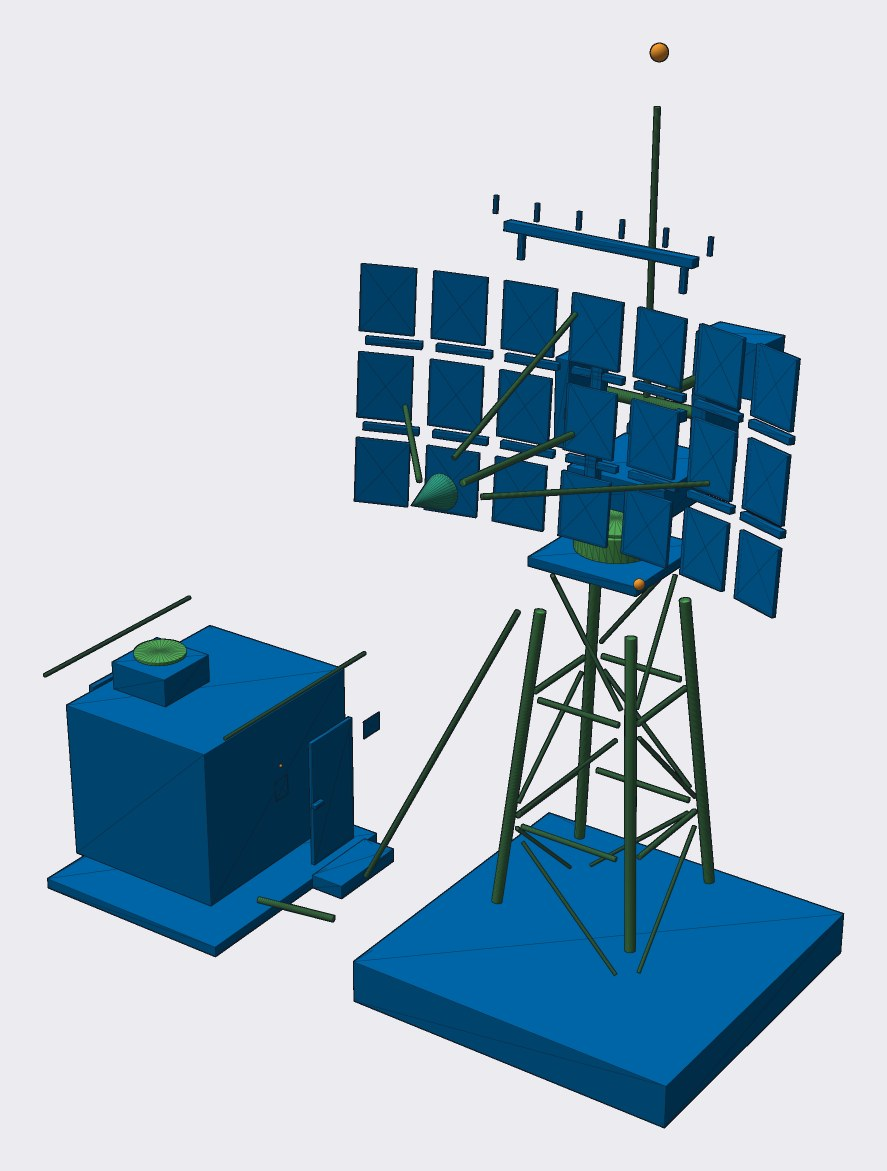
\includegraphics[width=4.24cm]{figures/img/shapes/air_defence_radar_prims.jpg}};
\node[anchor=west,inner sep=1pt] (L0) at (4.49,2.80) {Antenna array};
\draw[black!70,line width=0.4pt] (L0.west) -- (2.77,3.55); \fill[black] (2.77,3.55) circle (0.6pt);
\end{tikzpicture}\\[-0.3mm]{\fontsize{7.5}{9}\selectfont Full model} & {\fontsize{7.5}{9}\selectfont Made of primitives (pulled apart)}\end{tabular}
\\[0.8mm]{\fontsize{7}{8.5}\selectfont \primchipn{cuboid}{62}\quad \primchipn{sphere}{3}\quad \primchipn{cylinder}{42}\quad \primchipn{cone}{1}\quad \textbf{total 108}}\vspace{0.6mm}\end{minipage}}
\captionof{figure}{Air-defence radar.}\label{fig:d-air_defence_radar}
\end{center}\vspace{-3mm}
\noindent\textbf{Air-defence radar.}\label{des:air_defence_radar} Surveillance radar site (user-controllable). One instance, 29\,m east of the bunker. Placement of the first: $T(29.00,\,-0.30,\,-3.00)\,R_y(0^\circ)\,S(1)$.
{\fontsize{7}{8.2}\selectfont\setlength{\tabcolsep}{2.6pt}\renewcommand{\arraystretch}{1.02}
\begin{longtable}{@{}>{\raggedright\arraybackslash}p{3.3cm}l>{\raggedright\arraybackslash}p{2.7cm}>{\raggedright\arraybackslash}p{4.2cm}>{\raggedright\arraybackslash}p{2.3cm}>{\raggedright\arraybackslash}p{2.4cm}@{}}
\toprule Part ($\times n$) & Shape & Size $S$ (cm) & Position $T$ (cm, design frame) & Rotation $R$ ($^\circ$) & Parent\\\midrule\endhead
\bottomrule\endfoot
\multicolumn{6}{@{}l}{\textit{Air-defence radar}}\\[0.2mm]
Concrete plinth & \primchip{cuboid} & $460{\times}60{\times}460$ & $(0,\,30,\,0)$ & -- & root\\
Mast leg $\times$4 & \primchip{cylinder} & $14{\times}14{\times}408$ & $(\pm 62,\,263,\,\pm 62)$ & $(-83,\,\pm(45{+}90i),\,0)$ & root\\
Mast ring bar $\times$12 & \primchip{cylinder} & $7{\times}7{\times}90..137$ & $(-68..68,\,195{+}135i,\,-68..68)$ & $(0,\,-90{+}90i,\,0)$ & root\\
Mast brace $\times$12 & \primchip{cylinder} & $5{\times}5{\times}169..201$ & $(-74..74,\,128{+}135i,\,-74..74)$ & $(\pm(42{+}5i),\,-176..175,\,0)$ & root\\
Mast platform & \primchip{cuboid} & $150{\times}12{\times}150$ & $(0,\,470,\,0)$ & -- & root\\
Bearing housing & \primchip{cylinder} & $100{\times}100{\times}30$ & $(0,\,490,\,0)$ & $(90,\,0,\,0)$ & root\\
On-air lamp & \primchip{sphere} & $14{\times}14{\times}14$ & $(65,\,482,\,65)$ & -- & root\\
Equipment shelter & \primchip{cuboid} & $240{\times}230{\times}300$ & $(-460,\,130,\,50)$ & -- & root\\
Shelter slab & \primchip{cuboid} & $300{\times}15{\times}360$ & $(-460,\,8,\,50)$ & -- & root\\
Shelter door & \primchip{cuboid} & $6{\times}190{\times}90$ & $(-337,\,110,\,0)$ & -- & root\\
Door handle & \primchip{cuboid} & $8{\times}6{\times}20$ & $(-332,\,110,\,30)$ & -- & root\\
Door step & \primchip{cuboid} & $50{\times}20{\times}120$ & $(-310,\,25,\,0)$ & -- & root\\
Lit vent & \primchip{cuboid} & $8{\times}30{\times}90$ & $(-583,\,190,\,60)$ & -- & root\\
Roof air conditioner & \primchip{cuboid} & $90{\times}40{\times}90$ & $(-460,\,265,\,120)$ & -- & root\\
AC fan & \primchip{cylinder} & $70{\times}70{\times}5$ & $(-460,\,287,\,120)$ & $(90,\,0,\,0)$ & root\\
Power cable & \primchip{cylinder} & $9{\times}9{\times}112$ & $(-285,\,50,\,130)$ & $(0,\,100,\,0)$ & root\\
Mast cable duct & \primchip{cylinder} & $7{\times}7{\times}445$ & $(-140,\,260,\,83)$ & $(-64,\,113,\,0)$ & root\\
Shelter status display & \primchip{cuboid} & $1.2{\times}30{\times}26$ & $(-339,\,150,\,80)$ & -- & root\\
Shelter status LED & \primchip{sphere} & $5{\times}5{\times}5$ & $(-340,\,176,\,80)$ & -- & root\\
Door placard & \primchip{cuboid} & $1.2{\times}26{\times}36$ & $(-339,\,155,\,-75)$ & -- & root\\
Shelter roof edge $\times$2 & \primchip{cylinder} & $5{\times}5{\times}300$ & $(\{-580,-340\},\,245,\,50)$ & -- & root\\
Bearing seal & \primchip{cylinder} & $104{\times}104{\times}4$ & $(0,\,506,\,0)$ & $(90,\,0,\,0)$ & root\\
\multicolumn{6}{@{}l}{\textit{Azimuth head}}\\[0.2mm]
Pedestal & \primchip{cuboid} & $130{\times}40{\times}130$ & $(0,\,520,\,0)$ & -- & Azimuth head\\
Yoke cheek left & \primchip{cuboid} & $18{\times}110{\times}80$ & $(70,\,585,\,0)$ & -- & Azimuth head\\
Yoke cheek right & \primchip{cuboid} & $18{\times}110{\times}80$ & $(-70,\,585,\,0)$ & -- & Azimuth head\\
Beacon pole & \primchip{cylinder} & $7{\times}7{\times}360$ & $(0,\,720,\,0)$ & $(90,\,0,\,0)$ & Azimuth head\\
Aviation light & \primchip{sphere} & $20{\times}20{\times}20$ & $(0,\,905,\,0)$ & -- & Azimuth head\\
Trunnion & \primchip{cylinder} & $14{\times}14{\times}150$ & $(0,\,590,\,0)$ & $(0,\,90,\,0)$ & Elevation yoke\\
Array tile c1 r1 & \primchip{cuboid} & $64{\times}78{\times}5$ & $(-191,\,520,\,143)$ & $(0,\,22,\,0)$ & Antenna array\\
Array tile c1 r2 & \primchip{cuboid} & $64{\times}78{\times}5$ & $(-191,\,600,\,138)$ & $(0,\,22,\,0)$ & Antenna array\\
Array tile c1 r3 & \primchip{cuboid} & $64{\times}78{\times}5$ & $(-191,\,679,\,132)$ & $(0,\,22,\,0)$ & Antenna array\\
Antenna rib $\times$14 & \primchip{cuboid} & $66{\times}8{\times}8$ & $(-188..188,\,557..639,\,89..133)$ & $(0,\,\pm(0{+}8i),\,0)$ & Antenna array\\
Array tile c2 r1 & \primchip{cuboid} & $64{\times}78{\times}5$ & $(-129,\,518,\,122)$ & $(0,\,15,\,0)$ & Antenna array\\
Array tile c2 r2 & \primchip{cuboid} & $64{\times}78{\times}5$ & $(-129,\,598,\,117)$ & $(0,\,15,\,0)$ & Antenna array\\
Array tile c2 r3 & \primchip{cuboid} & $64{\times}78{\times}5$ & $(-129,\,678,\,111)$ & $(0,\,15,\,0)$ & Antenna array\\
Array tile c3 r1 & \primchip{cuboid} & $64{\times}78{\times}5$ & $(-65,\,517,\,110)$ & $(0,\,8,\,0)$ & Antenna array\\
Array tile c3 r2 & \primchip{cuboid} & $64{\times}78{\times}5$ & $(-65,\,597,\,104)$ & $(0,\,8,\,0)$ & Antenna array\\
Array tile c3 r3 & \primchip{cuboid} & $64{\times}78{\times}5$ & $(-65,\,677,\,98)$ & $(0,\,8,\,0)$ & Antenna array\\
Array tile c4 r1 & \primchip{cuboid} & $64{\times}78{\times}5$ & $(0,\,517,\,105)$ & -- & Antenna array\\
Array tile c4 r2 & \primchip{cuboid} & $64{\times}78{\times}5$ & $(0,\,597,\,100)$ & -- & Antenna array\\
Array tile c4 r3 & \primchip{cuboid} & $64{\times}78{\times}5$ & $(0,\,677,\,94)$ & -- & Antenna array\\
Array tile c5 r1 & \primchip{cuboid} & $64{\times}78{\times}5$ & $(65,\,517,\,110)$ & $(0,\,-8,\,0)$ & Antenna array\\
Array tile c5 r2 & \primchip{cuboid} & $64{\times}78{\times}5$ & $(65,\,597,\,104)$ & $(0,\,-8,\,0)$ & Antenna array\\
Array tile c5 r3 & \primchip{cuboid} & $64{\times}78{\times}5$ & $(65,\,677,\,98)$ & $(0,\,-8,\,0)$ & Antenna array\\
Array tile c6 r1 & \primchip{cuboid} & $64{\times}78{\times}5$ & $(129,\,518,\,122)$ & $(0,\,-15,\,0)$ & Antenna array\\
Array tile c6 r2 & \primchip{cuboid} & $64{\times}78{\times}5$ & $(129,\,598,\,117)$ & $(0,\,-15,\,0)$ & Antenna array\\
Array tile c6 r3 & \primchip{cuboid} & $64{\times}78{\times}5$ & $(129,\,678,\,111)$ & $(0,\,-15,\,0)$ & Antenna array\\
Array tile c7 r1 & \primchip{cuboid} & $64{\times}78{\times}5$ & $(191,\,520,\,143)$ & $(0,\,-22,\,0)$ & Antenna array\\
Array tile c7 r2 & \primchip{cuboid} & $64{\times}78{\times}5$ & $(191,\,600,\,138)$ & $(0,\,-22,\,0)$ & Antenna array\\
Array tile c7 r3 & \primchip{cuboid} & $64{\times}78{\times}5$ & $(191,\,679,\,132)$ & $(0,\,-22,\,0)$ & Antenna array\\
Antenna spine & \primchip{cuboid} & $14{\times}260{\times}14$ & $(0,\,596,\,90)$ & -- & Antenna array\\
Arm left & \primchip{cuboid} & $12{\times}12{\times}91.2$ & $(38,\,593,\,45)$ & $(0,\,-9,\,0)$ & Elevation yoke\\
Arm right & \primchip{cuboid} & $12{\times}12{\times}91.2$ & $(-38,\,593,\,45)$ & $(0,\,9,\,0)$ & Elevation yoke\\
Feed horn & \primchip{cone} & $40{\times}40{\times}55$ & $(0,\,614,\,339)$ & -- & Elevation yoke\\
Feed waveguide & \primchip{cylinder} & $8{\times}8{\times}215$ & $(0,\,604,\,207)$ & -- & Elevation yoke\\
Feed strut left & \primchip{cylinder} & $6{\times}6{\times}251$ & $(91,\,606,\,232)$ & $(0,\,-39,\,0)$ & Elevation yoke\\
Feed strut right & \primchip{cylinder} & $6{\times}6{\times}251$ & $(-91,\,606,\,232)$ & $(0,\,39,\,0)$ & Elevation yoke\\
Feed strut top & \primchip{cylinder} & $6{\times}6{\times}250$ & $(0,\,671,\,212)$ & $(26,\,0,\,0)$ & Elevation yoke\\
Counterweight arm & \primchip{cylinder} & $12{\times}12{\times}130$ & $(0,\,585,\,-75)$ & $(0,\,180,\,0)$ & Elevation yoke\\
Counterweight & \primchip{cuboid} & $90{\times}70{\times}60$ & $(0,\,578,\,-170)$ & -- & Elevation yoke\\
IFF bar & \primchip{cuboid} & $240{\times}10{\times}14$ & $(0,\,759,\,88)$ & -- & Elevation yoke\\
IFF post left & \primchip{cuboid} & $6{\times}30{\times}6$ & $(80,\,741,\,85)$ & -- & Elevation yoke\\
IFF post right & \primchip{cuboid} & $6{\times}30{\times}6$ & $(-80,\,741,\,85)$ & -- & Elevation yoke\\
IFF dipole $\times$6 & \primchip{cuboid} & $4{\times}20{\times}4$ & $(\pm(21{+}42i),\,775,\,87)$ & -- & Elevation yoke\\
\end{longtable}}

\needspace{8.6cm}
\begin{center}
\fcolorbox{black!30}{white}{\begin{minipage}{0.975\linewidth}\centering\vspace{0.6mm}
\begin{tabular}{@{}c@{\hspace{3mm}}c@{}}\img{figures/img/shapes/motor_pool_model.jpg}{7.77cm} & \img{figures/img/shapes/motor_pool_prims.jpg}{8.83cm}\\[-0.3mm]{\fontsize{7.5}{9}\selectfont Full model} & {\fontsize{7.5}{9}\selectfont Made of primitives (pulled apart)}\end{tabular}
\\[0.8mm]{\fontsize{7}{8.5}\selectfont \primchipn{cuboid}{1}\quad \primchipn{sphere}{1}\quad \primchipn{cylinder}{2}\quad \textbf{total 4}\\pale: Camouflage net $\times$1 (55 parts), Cargo truck $\times$2 (62 parts), Container $\times$2 (22 parts)}\vspace{0.6mm}\end{minipage}}
\captionof{figure}{Motor pool.}\label{fig:d-motor_pool}
\end{center}\vspace{-3mm}
\noindent\textbf{Motor pool.}\label{des:motor_pool} Vehicle park around the tank spot. One instance, 27\,m south-west of the bunker. Placement of the first: $T(-22.00,\,-0.30,\,-16.00)\,R_y(0^\circ)\,S(1)$.
{\fontsize{7}{8.2}\selectfont\setlength{\tabcolsep}{2.6pt}\renewcommand{\arraystretch}{1.02}
\begin{longtable}{@{}>{\raggedright\arraybackslash}p{3.3cm}l>{\raggedright\arraybackslash}p{2.7cm}>{\raggedright\arraybackslash}p{4.2cm}>{\raggedright\arraybackslash}p{2.3cm}>{\raggedright\arraybackslash}p{2.4cm}@{}}
\toprule Part ($\times n$) & Shape & Size $S$ (cm) & Position $T$ (cm, design frame) & Rotation $R$ ($^\circ$) & Parent\\\midrule\endhead
\bottomrule\endfoot
Floodlight pole & \primchip{cylinder} & $16{\times}16{\times}520$ & $(0,\,260,\,792)$ & $(90,\,0,\,0)$ & root\\
Floodlight arm & \primchip{cuboid} & $10{\times}10{\times}50$ & $(0,\,530,\,792)$ & $(0,\,45,\,0)$ & root\\
Floodlight housing & \primchip{cylinder} & $42{\times}42{\times}36$ & $(0,\,540,\,792)$ & $(29,\,180,\,0)$ & root\\
Floodlight lens & \primchip{sphere} & $38{\times}38{\times}6$ & $(0,\,530,\,774)$ & $(29,\,180,\,0)$ & root\\
\textit{Container} $\times$2 & \multicolumn{5}{@{}l}{\textit{nested design, drawn pale; its parts are counted in its own card (Figure~\ref{fig:d-container})}}\\
\textit{Cargo truck} $\times$2 & \multicolumn{5}{@{}l}{\textit{nested design, drawn pale; its parts are counted in its own card (Figure~\ref{fig:d-cargo_truck})}}\\
\textit{Camouflage net} $\times$1 & \multicolumn{5}{@{}l}{\textit{nested design, drawn pale; its parts are counted in its own card (Figure~\ref{fig:d-camouflage_net})}}\\
\end{longtable}}

\needspace{8.6cm}
\begin{center}
\fcolorbox{black!30}{white}{\begin{minipage}{0.975\linewidth}\centering\vspace{0.6mm}
\begin{tabular}{@{}c@{\hspace{3mm}}c@{}}\img{figures/img/shapes/helipad_model.jpg}{5.93cm} & \img{figures/img/shapes/helipad_prims.jpg}{5.95cm}\\[-0.3mm]{\fontsize{7.5}{9}\selectfont Full model} & {\fontsize{7.5}{9}\selectfont Made of primitives (pulled apart)}\end{tabular}
\\[0.8mm]{\fontsize{7}{8.5}\selectfont \primchipn{cuboid}{31}\quad \primchipn{sphere}{17}\quad \primchipn{cylinder}{3}\quad \textbf{total 51}}\vspace{0.6mm}\end{minipage}}
\captionof{figure}{Helipad.}\label{fig:d-helipad}
\end{center}\vspace{-3mm}
\noindent\textbf{Helipad.}\label{des:helipad} Concrete landing pad with markings and lights. One instance, 26\,m north-east of the bunker. Placement of the first: $T(20.30,\,-0.30,\,17.00)\,R_y(0^\circ)\,S(1)$.
{\fontsize{7}{8.2}\selectfont\setlength{\tabcolsep}{2.6pt}\renewcommand{\arraystretch}{1.02}
\begin{longtable}{@{}>{\raggedright\arraybackslash}p{3.3cm}l>{\raggedright\arraybackslash}p{2.7cm}>{\raggedright\arraybackslash}p{4.2cm}>{\raggedright\arraybackslash}p{2.3cm}>{\raggedright\arraybackslash}p{2.4cm}@{}}
\toprule Part ($\times n$) & Shape & Size $S$ (cm) & Position $T$ (cm, design frame) & Rotation $R$ ($^\circ$) & Parent\\\midrule\endhead
\bottomrule\endfoot
Helipad disc & \primchip{cylinder} & $1e+03{\times}1e+03{\times}8$ & $(0,\,4,\,0)$ & $(90,\,0,\,0)$ & root\\
H bar $\times$2 & \primchip{cuboid} & $50{\times}1.2{\times}320$ & $(\pm 95,\,9,\,0)$ & -- & root\\
H crossbar & \primchip{cuboid} & $150{\times}1.2{\times}50$ & $(0,\,9,\,0)$ & -- & root\\
Circle mark $\times$24 & \primchip{cuboid} & $70{\times}1.2{\times}20$ & $(-390..390,\,9,\,-390..390)$ & $(0,\,-165{+}15i,\,0)$ & root\\
Edge mark $\times$4 & \primchip{cuboid} & $35{\times}1.2{\times}100$ & $(-460{+}460i,\,9,\,-460{+}460i)$ & $(0,\,90{+}90i,\,0)$ & root\\
Perimeter light $\times$16 & \primchip{sphere} & $20{\times}7{\times}20$ & $(-476..476,\,7,\,-476..476)$ & -- & root\\
Pad floodlight pole & \primchip{cylinder} & $14{\times}14{\times}400$ & $(-620,\,200,\,400)$ & $(90,\,0,\,0)$ & root\\
Pad floodlight housing & \primchip{cylinder} & $36{\times}36{\times}30$ & $(-620,\,420,\,400)$ & $(23,\,123,\,0)$ & root\\
Pad floodlight lens & \primchip{sphere} & $32{\times}32{\times}5$ & $(-607,\,413,\,392)$ & $(23,\,123,\,0)$ & root\\
\end{longtable}}

\needspace{8.6cm}
\begin{center}
\fcolorbox{black!30}{white}{\begin{minipage}{0.975\linewidth}\centering\vspace{0.6mm}
\begin{tabular}{@{}c@{\hspace{3mm}}c@{}}\img{figures/img/shapes/ammunition_bunker_cut_model.jpg}{5.08cm} & \img{figures/img/shapes/ammunition_bunker_cut_prims.jpg}{5.09cm}\\[-0.3mm]{\fontsize{7.5}{9}\selectfont Full model} & {\fontsize{7.5}{9}\selectfont Made of primitives (pulled apart)}\end{tabular}
\\[0.8mm]{\fontsize{7}{8.5}\selectfont \primchipn{cuboid}{12}\quad \primchipn{wedge}{2}\quad \primchipn{sphere}{10}\quad \primchipn{capsule}{8}\quad \primchipn{cylinder}{4}\quad \textbf{total 36}\\pale: Supply cache $\times$1 (7 parts)}\vspace{0.6mm}\end{minipage}}
\captionof{figure}{Ammunition bunker. Cutaway: earth mounds and turf clump are left out in both panels (8 parts) so what they cover shows.}\label{fig:d-ammunition_bunker}
\end{center}\vspace{-3mm}
\noindent\textbf{Ammunition bunker.}\label{des:ammunition_bunker} Earth-covered ammunition store; entrance towards local +Z. One instance, 28\,m north of the bunker. Placement of the first: $T(10.50,\,-0.30,\,26.20)\,R_y(-90^\circ)\,S(1)$.
{\fontsize{7}{8.2}\selectfont\setlength{\tabcolsep}{2.6pt}\renewcommand{\arraystretch}{1.02}
\begin{longtable}{@{}>{\raggedright\arraybackslash}p{3.3cm}l>{\raggedright\arraybackslash}p{2.7cm}>{\raggedright\arraybackslash}p{4.2cm}>{\raggedright\arraybackslash}p{2.3cm}>{\raggedright\arraybackslash}p{2.4cm}@{}}
\toprule Part ($\times n$) & Shape & Size $S$ (cm) & Position $T$ (cm, design frame) & Rotation $R$ ($^\circ$) & Parent\\\midrule\endhead
\bottomrule\endfoot
Concrete chamber & \primchip{cuboid} & $560{\times}130{\times}520$ & $(0,\,65,\,-40)$ & -- & root\\
Earth mound & \primchip{sphere} & $820{\times}440{\times}740$ & $(0,\,0,\,-40)$ & -- & root\\
Earth mound lobe $\times$2 & \primchip{sphere} & $380..420{\times}220..240{\times}300..340$ & $(\{-220,230\},\,10,\,\{-180,-120\})$ & $(0,\,\{-25,20\},\,0)$ & root\\
Turf clump $\times$5 & \primchip{sphere} & $100{\times}40{\times}90$ & $(\pm(0{+}90i),\,150{+}10i,\,-120{+}30i)$ & $(0,\,0{+}37i,\,0)$ & root\\
Headwall block $\times$2 & \primchip{cuboid} & $130{\times}190{\times}50$ & $(\pm 115,\,95,\,240)$ & -- & root\\
Headwall lintel & \primchip{cuboid} & $360{\times}40{\times}50$ & $(0,\,170,\,240)$ & -- & root\\
Blast door & \primchip{cuboid} & $100{\times}150{\times}12$ & $(0,\,75,\,220)$ & -- & root\\
Door frame stripe & \primchip{cuboid} & $120{\times}10{\times}14$ & $(0,\,155,\,220)$ & -- & root\\
Door step & \primchip{cuboid} & $140{\times}14{\times}50$ & $(0,\,7,\,285)$ & -- & root\\
Door step marker & \primchip{sphere} & $9{\times}4{\times}9$ & $(50,\,16,\,295)$ & -- & root\\
Door lamp hood & \primchip{cuboid} & $34{\times}4{\times}30$ & $(0,\,200,\,275)$ & -- & root\\
Door lamp & \primchip{sphere} & $16{\times}16{\times}6$ & $(0,\,193,\,275)$ & $(90,\,0,\,0)$ & root\\
Warning sign & \primchip{cuboid} & $50{\times}35{\times}3$ & $(-115,\,130,\,267)$ & -- & root\\
Wing wall core $\times$2 & \primchip{cuboid} & $60{\times}130{\times}240$ & $(\pm 200,\,65,\,350)$ & -- & root\\
Wing wall slope $\times$2 & \primchip{wedge} & $240{\times}130{\times}65$ & $(\{-263,262\},\,65,\,350)$ & $(0,\,\pm 90,\,0)$ & root\\
Wing sandbag $\times$8 & \primchip{capsule} & $28{\times}17{\times}50$ & $(\pm 200,\,138,\,250{+}60i)$ & $(0,\,90,\,0)$ & root\\
Blast baffle & \primchip{cuboid} & $260{\times}100{\times}50$ & $(0,\,50,\,540)$ & -- & root\\
Vent pipe $\times$2 & \primchip{cylinder} & $20{\times}20{\times}100$ & $(\pm 130,\,200,\,-100)$ & $(90,\,0,\,0)$ & root\\
Vent cap $\times$2 & \primchip{cylinder} & $34{\times}34{\times}6$ & $(\pm 130,\,255,\,-100)$ & $(90,\,0,\,0)$ & root\\
\textit{Supply cache} $\times$1 & \multicolumn{5}{@{}l}{\textit{nested design, drawn pale; its parts are counted in its own card (Figure~\ref{fig:d-supply_cache})}}\\
\end{longtable}}

\needspace{8.6cm}
\begin{center}
\fcolorbox{black!30}{white}{\begin{minipage}{0.975\linewidth}\centering\vspace{0.6mm}
\begin{tabular}{@{}c@{\hspace{3mm}}c@{}}\img{figures/img/shapes/guard_tower_model.jpg}{2.61cm} & \img{figures/img/shapes/guard_tower_prims.jpg}{2.38cm}\\[-0.3mm]{\fontsize{7.5}{9}\selectfont Full model} & {\fontsize{7.5}{9}\selectfont Made of primitives (pulled apart)}\end{tabular}
\\[0.8mm]{\fontsize{7}{8.5}\selectfont \primchipn{cuboid}{11}\quad \primchipn{sphere}{2}\quad \primchipn{cylinder}{24}\quad \textbf{total 37}}\vspace{0.6mm}\end{minipage}}
\captionof{figure}{Guard tower.}\label{fig:d-guard_tower}
\end{center}\vspace{-3mm}
\noindent\textbf{Guard tower.}\label{des:guard_tower} Perimeter guard tower; local +Z points into the base. 4 instances; the first stands 32\,m north-east of the bunker. Placement of the first: $T(16.20,\,-0.30,\,28.06)\,R_y(-150^\circ)\,S(1)$.
{\fontsize{7}{8.2}\selectfont\setlength{\tabcolsep}{2.6pt}\renewcommand{\arraystretch}{1.02}
\begin{longtable}{@{}>{\raggedright\arraybackslash}p{3.3cm}l>{\raggedright\arraybackslash}p{2.7cm}>{\raggedright\arraybackslash}p{4.2cm}>{\raggedright\arraybackslash}p{2.3cm}>{\raggedright\arraybackslash}p{2.4cm}@{}}
\toprule Part ($\times n$) & Shape & Size $S$ (cm) & Position $T$ (cm, design frame) & Rotation $R$ ($^\circ$) & Parent\\\midrule\endhead
\bottomrule\endfoot
Tower leg $\times$4 & \primchip{cylinder} & $16{\times}16{\times}420$ & $(\pm 109,\,190,\,\pm 109)$ & $(-88,\,\pm(45{+}90i),\,0)$ & root\\
Tower brace $\times$4 & \primchip{cylinder} & $7{\times}7{\times}380$ & $(\pm(5{+}104i),\,185,\,\pm(5{+}104i))$ & $(-55,\,-178{+}90i,\,0)$ & root\\
Platform & \primchip{cuboid} & $290{\times}14{\times}290$ & $(0,\,407,\,0)$ & -- & root\\
Parapet front & \primchip{cuboid} & $290{\times}95{\times}50$ & $(0,\,462,\,120)$ & -- & root\\
Parapet side $\times$2 & \primchip{cuboid} & $50{\times}95{\times}200$ & $(\pm 120,\,462,\,0)$ & -- & root\\
Parapet cap & \primchip{cuboid} & $290{\times}14{\times}50$ & $(0,\,517,\,120)$ & -- & root\\
Roof post $\times$4 & \primchip{cylinder} & $10{\times}10{\times}210$ & $(\pm 135,\,519,\,\pm 135)$ & $(90,\,0,\,0)$ & root\\
Roof slab & \primchip{cuboid} & $350{\times}10{\times}350$ & $(0,\,630,\,0)$ & -- & root\\
Roof lip & \primchip{cuboid} & $350{\times}12{\times}8$ & $(0,\,638,\,170)$ & -- & root\\
Ladder rail $\times$2 & \primchip{cylinder} & $5{\times}5{\times}422$ & $(\pm 25,\,190,\,-167)$ & $(-84,\,0,\,0)$ & root\\
Ladder rung $\times$5 & \primchip{cylinder} & $3.5{\times}3.5{\times}50$ & $(0,\,33{+}77i,\,-184{+}8i)$ & $(0,\,90,\,0)$ & root\\
MG mount & \primchip{cuboid} & $12{\times}30{\times}12$ & $(50,\,535,\,115)$ & -- & root\\
MG receiver & \primchip{cuboid} & $14{\times}16{\times}50$ & $(50,\,558,\,120)$ & -- & root\\
MG barrel & \primchip{cylinder} & $4{\times}4{\times}70$ & $(50,\,558,\,172)$ & -- & root\\
Floodlight bracket & \primchip{cylinder} & $6{\times}6{\times}25$ & $(-80,\,618,\,162)$ & $(90,\,0,\,0)$ & root\\
Floodlight housing & \primchip{cylinder} & $36{\times}36{\times}34$ & $(-80,\,605,\,162)$ & $(27,\,2,\,0)$ & root\\
Floodlight lens & \primchip{sphere} & $32{\times}32{\times}6$ & $(-80,\,597,\,178)$ & $(27,\,2,\,0)$ & root\\
Sandbag course $\times$2 & \primchip{cylinder} & $10{\times}10{\times}280$ & $(0,\,\{436,476\},\,145)$ & $(0,\,90,\,0)$ & root\\
MG ammo box & \primchip{cuboid} & $26{\times}18{\times}12$ & $(80,\,533,\,115)$ & -- & root\\
Field radio & \primchip{cuboid} & $30{\times}35{\times}15$ & $(-85,\,432,\,85)$ & -- & root\\
Radio LED & \primchip{sphere} & $3.5{\times}3.5{\times}2$ & $(-85,\,442,\,77)$ & -- & root\\
\end{longtable}}

\needspace{8.6cm}
\begin{center}
\fcolorbox{black!30}{white}{\begin{minipage}{0.975\linewidth}\centering\vspace{0.6mm}
\begin{tabular}{@{}c@{\hspace{3mm}}c@{}}\img{figures/img/shapes/watchtower_model.jpg}{2.13cm} & \img{figures/img/shapes/watchtower_prims.jpg}{1.93cm}\\[-0.3mm]{\fontsize{7.5}{9}\selectfont Full model} & {\fontsize{7.5}{9}\selectfont Made of primitives (pulled apart)}\end{tabular}
\\[0.8mm]{\fontsize{7}{8.5}\selectfont \primchipn{cuboid}{5}\quad \primchipn{sphere}{1}\quad \primchipn{cylinder}{19}\quad \primchipn{cone}{1}\quad \textbf{total 26}}\vspace{0.6mm}\end{minipage}}
\captionof{figure}{Watchtower.}\label{fig:d-watchtower}
\end{center}\vspace{-3mm}
\noindent\textbf{Watchtower.}\label{des:watchtower} Guard tower with floodlight. One instance, 14\,m north-east of the bunker. Placement of the first: $T(10.50,\,0.06,\,10.00)\,R_y(0^\circ)\,S(1)$.
{\fontsize{7}{8.2}\selectfont\setlength{\tabcolsep}{2.6pt}\renewcommand{\arraystretch}{1.02}
\begin{longtable}{@{}>{\raggedright\arraybackslash}p{3.3cm}l>{\raggedright\arraybackslash}p{2.7cm}>{\raggedright\arraybackslash}p{4.2cm}>{\raggedright\arraybackslash}p{2.3cm}>{\raggedright\arraybackslash}p{2.4cm}@{}}
\toprule Part ($\times n$) & Shape & Size $S$ (cm) & Position $T$ (cm, design frame) & Rotation $R$ ($^\circ$) & Parent\\\midrule\endhead
\bottomrule\endfoot
Tower leg $\times$4 & \primchip{cylinder} & $14{\times}14{\times}531$ & $(\pm 95,\,235,\,\pm 95)$ & $(-87,\,\pm(45{+}90i),\,0)$ & root\\
Tower brace $\times$4 & \primchip{cylinder} & $8{\times}8{\times}342$ & $(\pm(5{+}93i),\,160,\,\pm(5{+}93i))$ & $(-55,\,-177{+}90i,\,0)$ & root\\
Platform & \primchip{cuboid} & $240{\times}12{\times}240$ & $(0,\,310,\,0)$ & -- & root\\
Parapet front & \primchip{cuboid} & $230{\times}90{\times}6$ & $(0,\,361,\,-112)$ & -- & root\\
Parapet side $\times$2 & \primchip{cuboid} & $6{\times}90{\times}230$ & $(\pm 112,\,361,\,0)$ & -- & root\\
Hand rail & \primchip{cylinder} & $5{\times}5{\times}220$ & $(0,\,400,\,112)$ & $(0,\,90,\,0)$ & root\\
Roof slab & \primchip{cuboid} & $250{\times}8{\times}250$ & $(0,\,502,\,0)$ & -- & root\\
Roof cone & \primchip{cone} & $340{\times}340{\times}90$ & $(0,\,551,\,0)$ & $(-90,\,45,\,0)$ & root\\
Ladder rail $\times$2 & \primchip{cylinder} & $5{\times}5{\times}337$ & $(\pm 25,\,147,\,127)$ & $(-84,\,180,\,0)$ & root\\
Ladder rung $\times$6 & \primchip{cylinder} & $3.5{\times}3.5{\times}50$ & $(0,\,16{+}52i,\,113{+}5i)$ & $(0,\,90,\,0)$ & root\\
Floodlight bracket & \primchip{cylinder} & $6{\times}6{\times}44$ & $(-95,\,428,\,-95)$ & $(90,\,0,\,0)$ & root\\
Floodlight housing & \primchip{cylinder} & $34{\times}34{\times}32$ & $(-95,\,466,\,-95)$ & $(26,\,-134,\,0)$ & root\\
Floodlight lens & \primchip{sphere} & $30{\times}30{\times}6$ & $(-106,\,459,\,-106)$ & $(26,\,-134,\,0)$ & root\\
\end{longtable}}

\needspace{8.6cm}
\begin{center}
\fcolorbox{black!30}{white}{\begin{minipage}{0.975\linewidth}\centering\vspace{0.6mm}
\begin{tabular}{@{}c@{\hspace{3mm}}c@{}}\img{figures/img/shapes/fuel_depot_model.jpg}{8.34cm} & \img{figures/img/shapes/fuel_depot_prims.jpg}{8.26cm}\\[-0.3mm]{\fontsize{7.5}{9}\selectfont Full model} & {\fontsize{7.5}{9}\selectfont Made of primitives (pulled apart)}\end{tabular}
\\[0.8mm]{\fontsize{7}{8.5}\selectfont \primchipn{cuboid}{8}\quad \primchipn{sphere}{2}\quad \primchipn{cylinder}{10}\quad \textbf{total 20}}\vspace{0.6mm}\end{minipage}}
\captionof{figure}{Fuel depot.}\label{fig:d-fuel_depot}
\end{center}\vspace{-3mm}
\noindent\textbf{Fuel depot.}\label{des:fuel_depot} Bladders in a sandbag dike, pump, generator. One instance, 29\,m south of the bunker. Placement of the first: $T(-6.00,\,-0.30,\,-28.50)\,R_y(0^\circ)\,S(1)$.
{\fontsize{7}{8.2}\selectfont\setlength{\tabcolsep}{2.6pt}\renewcommand{\arraystretch}{1.02}
\begin{longtable}{@{}>{\raggedright\arraybackslash}p{3.3cm}l>{\raggedright\arraybackslash}p{2.7cm}>{\raggedright\arraybackslash}p{4.2cm}>{\raggedright\arraybackslash}p{2.3cm}>{\raggedright\arraybackslash}p{2.4cm}@{}}
\toprule Part ($\times n$) & Shape & Size $S$ (cm) & Position $T$ (cm, design frame) & Rotation $R$ ($^\circ$) & Parent\\\midrule\endhead
\bottomrule\endfoot
\multicolumn{6}{@{}l}{\textit{Fuel depot}}\\[0.2mm]
Dike wall $\times$4 & \primchip{cuboid} & $50..840{\times}55{\times}50..500$ & $(-400{+}400i,\,28,\,-250{+}250i)$ & -- & root\\
Fuel bladder $\times$2 & \primchip{sphere} & $340{\times}110{\times}210$ & $(\pm 200,\,50,\,30)$ & -- & root\\
Bladder fill cap $\times$2 & \primchip{cylinder} & $25{\times}25{\times}10$ & $(\pm 200,\,102,\,30)$ & $(90,\,0,\,0)$ & root\\
Pump skid & \primchip{cuboid} & $90{\times}40{\times}60$ & $(0,\,20,\,-170)$ & -- & root\\
Fuel hose $\times$2 & \primchip{cylinder} & $8{\times}8{\times}189$ & $(\pm 120,\,45,\,-120)$ & $(-3,\,\pm 58,\,0)$ & root\\
Fuel drum $\times$4 & \primchip{cylinder} & $55{\times}55{\times}85$ & $(-320{+}60i,\,43,\,-360)$ & $(90,\,0,\,0)$ & root\\
\multicolumn{6}{@{}l}{\textit{Generator}}\\[0.2mm]
Generator housing & \primchip{cuboid} & $100{\times}110{\times}200$ & $(720,\,70,\,-60)$ & -- & Generator\\
Generator skid & \primchip{cuboid} & $120{\times}15{\times}220$ & $(720,\,7,\,-60)$ & -- & Generator\\
Exhaust stack & \primchip{cylinder} & $10{\times}10{\times}70$ & $(800,\,160,\,-90)$ & $(90,\,0,\,0)$ & Generator\\
Control panel & \primchip{cuboid} & $50{\times}40{\times}4$ & $(823,\,85,\,-60)$ & -- & Generator\\
Power cable & \primchip{cylinder} & $6{\times}6{\times}230$ & $(945,\,12,\,-60)$ & $(4,\,0,\,0)$ & Generator\\
\end{longtable}}

\needspace{8.6cm}
\begin{center}
\fcolorbox{black!30}{white}{\begin{minipage}{0.975\linewidth}\centering\vspace{0.6mm}
\begin{tabular}{@{}c@{\hspace{3mm}}c@{}}\img{figures/img/shapes/quonset_hut_model.jpg}{4.86cm} & \img{figures/img/shapes/quonset_hut_prims.jpg}{4.70cm}\\[-0.3mm]{\fontsize{7.5}{9}\selectfont Full model} & {\fontsize{7.5}{9}\selectfont Made of primitives (pulled apart)}\end{tabular}
\\[0.8mm]{\fontsize{7}{8.5}\selectfont \primchipn{cuboid}{14}\quad \primchipn{sphere}{2}\quad \primchipn{cylinder}{3}\quad \textbf{total 19}}\vspace{0.6mm}\end{minipage}}
\captionof{figure}{Quonset hut.}\label{fig:d-quonset_hut}
\end{center}\vspace{-3mm}
\noindent\textbf{Quonset hut.}\label{des:quonset_hut} Half-buried cylinder hut; local +Z faces the compound. 3 instances; the first stands 27\,m north-west of the bunker. Placement of the first: $T(-22.03,\,-0.30,\,15.61)\,R_y(125^\circ)\,S(1)$.
{\fontsize{7}{8.2}\selectfont\setlength{\tabcolsep}{2.6pt}\renewcommand{\arraystretch}{1.02}
\begin{longtable}{@{}>{\raggedright\arraybackslash}p{3.3cm}l>{\raggedright\arraybackslash}p{2.7cm}>{\raggedright\arraybackslash}p{4.2cm}>{\raggedright\arraybackslash}p{2.3cm}>{\raggedright\arraybackslash}p{2.4cm}@{}}
\toprule Part ($\times n$) & Shape & Size $S$ (cm) & Position $T$ (cm, design frame) & Rotation $R$ ($^\circ$) & Parent\\\midrule\endhead
\bottomrule\endfoot
Hut shell & \primchip{cylinder} & $440{\times}440{\times}850$ & $(0,\,15,\,0)$ & -- & root\\
Hut door & \primchip{cuboid} & $95{\times}190{\times}8$ & $(-50,\,95,\,428)$ & -- & root\\
Hut door step & \primchip{cuboid} & $120{\times}18{\times}60$ & $(-50,\,9,\,458)$ & -- & root\\
Hut window & \primchip{cuboid} & $70{\times}50{\times}8$ & $(95,\,135,\,428)$ & -- & root\\
Hut AC unit & \primchip{cuboid} & $90{\times}60{\times}40$ & $(90,\,75,\,-448)$ & -- & root\\
Hut AC fan & \primchip{cylinder} & $45{\times}45{\times}5$ & $(90,\,75,\,-471)$ & -- & root\\
Hut flank window $\times$6 & \primchip{cuboid} & $70{\times}3{\times}50$ & $(\pm 187,\,132,\,-240{+}240i)$ & $(0,\,0,\,\pm 58)$ & root\\
Hut door lamp hood & \primchip{cuboid} & $30{\times}4{\times}26$ & $(-50,\,220,\,444)$ & -- & root\\
Hut door lamp & \primchip{sphere} & $14{\times}14{\times}6$ & $(-50,\,213,\,444)$ & $(90,\,0,\,0)$ & root\\
Door step marker & \primchip{sphere} & $9{\times}4{\times}9$ & $(-10,\,20,\,483)$ & -- & root\\
Hut stove pipe & \primchip{cylinder} & $12{\times}12{\times}80$ & $(-60,\,240,\,-150)$ & $(90,\,0,\,0)$ & root\\
Blast wall course $\times$3 & \primchip{cuboid} & $240..300{\times}40{\times}60$ & $(0,\,20{+}40i,\,628)$ & -- & root\\
\end{longtable}}

\needspace{8.6cm}
\begin{center}
\fcolorbox{black!30}{white}{\begin{minipage}{0.975\linewidth}\centering\vspace{0.6mm}
\begin{tabular}{@{}c@{\hspace{3mm}}c@{}}\img{figures/img/shapes/radio_mast_model.jpg}{1.81cm} & \img{figures/img/shapes/radio_mast_prims.jpg}{1.81cm}\\[-0.3mm]{\fontsize{7.5}{9}\selectfont Full model} & {\fontsize{7.5}{9}\selectfont Made of primitives (pulled apart)}\end{tabular}
\\[0.8mm]{\fontsize{7}{8.5}\selectfont \primchipn{cuboid}{5}\quad \primchipn{sphere}{2}\quad \primchipn{cylinder}{13}\quad \textbf{total 20}}\vspace{0.6mm}\end{minipage}}
\captionof{figure}{Radio mast.}\label{fig:d-radio_mast}
\end{center}\vspace{-3mm}
\noindent\textbf{Radio mast.}\label{des:radio_mast} Guyed lattice mast. One instance, 14\,m north-west of the bunker. Placement of the first: $T(-13.00,\,0.00,\,6.00)\,R_y(0^\circ)\,S(1)$.
{\fontsize{7}{8.2}\selectfont\setlength{\tabcolsep}{2.6pt}\renewcommand{\arraystretch}{1.02}
\begin{longtable}{@{}>{\raggedright\arraybackslash}p{3.3cm}l>{\raggedright\arraybackslash}p{2.7cm}>{\raggedright\arraybackslash}p{4.2cm}>{\raggedright\arraybackslash}p{2.3cm}>{\raggedright\arraybackslash}p{2.4cm}@{}}
\toprule Part ($\times n$) & Shape & Size $S$ (cm) & Position $T$ (cm, design frame) & Rotation $R$ ($^\circ$) & Parent\\\midrule\endhead
\bottomrule\endfoot
Mast footing & \primchip{cuboid} & $130{\times}20{\times}130$ & $(0,\,2,\,0)$ & -- & root\\
Equipment shelter & \primchip{cuboid} & $110{\times}100{\times}90$ & $(150,\,45,\,20)$ & -- & root\\
Mast leg $\times$3 & \primchip{cylinder} & $7{\times}7{\times}900$ & $(-23{+}23i,\,450,\,\{-14,-13,27\})$ & $(-88,\,-60{+}120i,\,0)$ & root\\
Mast brace $\times$6 & \primchip{cylinder} & $4{\times}4{\times}143..154$ & $(-15..13,\,110{+}140i,\,-16..11)$ & $(-78{+}2i,\,-153..88,\,0)$ & root\\
Whip antenna & \primchip{cylinder} & $3{\times}3{\times}140$ & $(0,\,970,\,0)$ & $(90,\,0,\,0)$ & root\\
Aviation light $\times$2 & \primchip{sphere} & $15..18{\times}15..18{\times}15..18$ & $(0,\,\{460,905\},\,0)$ & -- & root\\
Guy wire $\times$3 & \primchip{cylinder} & $1.5{\times}1.5{\times}746$ & $(-156{+}156i,\,\{354,356,373\},\,\{-180,90\})$ & $(61{+}1i,\,-60{+}120i,\,0)$ & root\\
Guy anchor $\times$3 & \primchip{cuboid} & $30{\times}25{\times}30$ & $(-312{+}312i,\,\{3,8,42\},\,\{-360,180\})$ & -- & root\\
\end{longtable}}

\needspace{8.6cm}
\begin{center}
\fcolorbox{black!30}{white}{\begin{minipage}{0.975\linewidth}\centering\vspace{0.6mm}
\begin{tabular}{@{}c@{\hspace{3mm}}c@{}}\img{figures/img/shapes/camouflaged_tent_model.jpg}{5.04cm} & \img{figures/img/shapes/camouflaged_tent_prims.jpg}{5.31cm}\\[-0.3mm]{\fontsize{7.5}{9}\selectfont Full model} & {\fontsize{7.5}{9}\selectfont Made of primitives (pulled apart)}\end{tabular}
\\[0.8mm]{\fontsize{7}{8.5}\selectfont \primchipn{cuboid}{3}\quad \primchipn{sphere}{4}\quad \primchipn{cylinder}{7}\quad \textbf{total 14}}\vspace{0.6mm}\end{minipage}}
\captionof{figure}{Camouflaged tent.}\label{fig:d-camouflaged_tent}
\end{center}\vspace{-3mm}
\noindent\textbf{Camouflaged tent.}\label{des:camouflaged_tent} A-frame tent under a net. One instance, 10\,m west of the bunker. Placement of the first: $T(-9.20,\,-0.15,\,-3.80)\,R_y(20^\circ)\,S(1)$.
{\fontsize{7}{8.2}\selectfont\setlength{\tabcolsep}{2.6pt}\renewcommand{\arraystretch}{1.02}
\begin{longtable}{@{}>{\raggedright\arraybackslash}p{3.3cm}l>{\raggedright\arraybackslash}p{2.7cm}>{\raggedright\arraybackslash}p{4.2cm}>{\raggedright\arraybackslash}p{2.3cm}>{\raggedright\arraybackslash}p{2.4cm}@{}}
\toprule Part ($\times n$) & Shape & Size $S$ (cm) & Position $T$ (cm, design frame) & Rotation $R$ ($^\circ$) & Parent\\\midrule\endhead
\bottomrule\endfoot
Ridge pole & \primchip{cylinder} & $7{\times}7{\times}320$ & $(0,\,170,\,0)$ & $(0,\,90,\,0)$ & root\\
Tent pole $\times$2 & \primchip{cylinder} & $7{\times}7{\times}190$ & $(\pm 150,\,75,\,0)$ & $(90,\,0,\,0)$ & root\\
Tent roof $\times$2 & \primchip{cuboid} & $310{\times}4{\times}185$ & $(0,\,98,\,\pm 58)$ & $(52,\,\{0,180\},\,0)$ & root\\
Tent back wall & \primchip{cuboid} & $4{\times}120{\times}120$ & $(-155,\,85,\,0)$ & $(45,\,0,\,0)$ & root\\
Camo net $\times$3 & \primchip{sphere} & $220..460{\times}60..100{\times}200..380$ & $(\{-120,0,130\},\,155{+}3i,\,\{-70,0,60\})$ & $(0,\,\{-20,0,25\},\,0)$ & root\\
Net pole $\times$4 & \primchip{cylinder} & $5{\times}5{\times}160$ & $(\pm 210,\,60,\,\pm 170)$ & $(90,\,0,\,0)$ & root\\
Lantern & \primchip{sphere} & $12{\times}16{\times}12$ & $(90,\,142,\,0)$ & -- & root\\
\end{longtable}}

\needspace{8.6cm}
\begin{center}
\fcolorbox{black!30}{white}{\begin{minipage}{0.975\linewidth}\centering\vspace{0.6mm}
\begin{tabular}{@{}c@{\hspace{3mm}}c@{}}\img{figures/img/shapes/container_model.jpg}{4.04cm} & \img{figures/img/shapes/container_prims.jpg}{4.05cm}\\[-0.3mm]{\fontsize{7.5}{9}\selectfont Full model} & {\fontsize{7.5}{9}\selectfont Made of primitives (pulled apart)}\end{tabular}
\\[0.8mm]{\fontsize{7}{8.5}\selectfont \primchipn{cube}{6}\quad \primchipn{cuboid}{3}\quad \primchipn{cylinder}{2}\quad \textbf{total 11}}\vspace{0.6mm}\end{minipage}}
\captionof{figure}{Container.}\label{fig:d-container}
\end{center}\vspace{-3mm}
\noindent\textbf{Container.}\label{des:container} ISO shipping container (20 ft). 2 instances; the first stands 30\,m west of the bunker, inside the motor pool. Placement of the first: $T(-28.08,\,-0.30,\,-11.33)\,R_y(45^\circ)\,S(1)$.
{\fontsize{7}{8.2}\selectfont\setlength{\tabcolsep}{2.6pt}\renewcommand{\arraystretch}{1.02}
\begin{longtable}{@{}>{\raggedright\arraybackslash}p{3.3cm}l>{\raggedright\arraybackslash}p{2.7cm}>{\raggedright\arraybackslash}p{4.2cm}>{\raggedright\arraybackslash}p{2.3cm}>{\raggedright\arraybackslash}p{2.4cm}@{}}
\toprule Part ($\times n$) & Shape & Size $S$ (cm) & Position $T$ (cm, design frame) & Rotation $R$ ($^\circ$) & Parent\\\midrule\endhead
\bottomrule\endfoot
Container body & \primchip{cuboid} & $244{\times}259{\times}606$ & $(0,\,129,\,0)$ & -- & root\\
Door bar $\times$2 & \primchip{cylinder} & $4.5{\times}4.5{\times}240$ & $(\pm 55,\,130,\,306)$ & $(90,\,0,\,0)$ & root\\
Door seam & \primchip{cuboid} & $3{\times}240{\times}3$ & $(0,\,130,\,306)$ & -- & root\\
Corner casting $\times$6 & \primchip{cube} & $18{\times}18{\times}18$ & $(\pm 115,\,\{9,255\},\,\pm 295)$ & -- & root\\
Container ID & \primchip{cuboid} & $1{\times}30{\times}140$ & $(123,\,220,\,160)$ & -- & root\\
\end{longtable}}

\needspace{8.6cm}
\begin{center}
\fcolorbox{black!30}{white}{\begin{minipage}{0.975\linewidth}\centering\vspace{0.6mm}
\begin{tabular}{@{}c@{\hspace{3mm}}c@{}}\img{figures/img/shapes/guard_booth_model.jpg}{3.04cm} & \img{figures/img/shapes/guard_booth_prims.jpg}{2.90cm}\\[-0.3mm]{\fontsize{7.5}{9}\selectfont Full model} & {\fontsize{7.5}{9}\selectfont Made of primitives (pulled apart)}\end{tabular}
\\[0.8mm]{\fontsize{7}{8.5}\selectfont \primchipn{cuboid}{8}\quad \primchipn{cylinder}{3}\quad \textbf{total 11}}\vspace{0.6mm}\end{minipage}}
\captionof{figure}{Guard booth.}\label{fig:d-guard_booth}
\end{center}\vspace{-3mm}
\noindent\textbf{Guard booth.}\label{des:guard_booth} Corrugated checkpoint booth. One instance, 32\,m north of the bunker, inside the outer gate. Placement of the first: $T(5.40,\,-0.30,\,31.60)\,R_y(0^\circ)\,S(1)$.
{\fontsize{7}{8.2}\selectfont\setlength{\tabcolsep}{2.6pt}\renewcommand{\arraystretch}{1.02}
\begin{longtable}{@{}>{\raggedright\arraybackslash}p{3.3cm}l>{\raggedright\arraybackslash}p{2.7cm}>{\raggedright\arraybackslash}p{4.2cm}>{\raggedright\arraybackslash}p{2.3cm}>{\raggedright\arraybackslash}p{2.4cm}@{}}
\toprule Part ($\times n$) & Shape & Size $S$ (cm) & Position $T$ (cm, design frame) & Rotation $R$ ($^\circ$) & Parent\\\midrule\endhead
\bottomrule\endfoot
Booth floor & \primchip{cuboid} & $240{\times}20{\times}240$ & $(0,\,10,\,0)$ & -- & root\\
Booth body & \primchip{cuboid} & $220{\times}230{\times}220$ & $(0,\,135,\,0)$ & -- & root\\
Booth roof & \primchip{cuboid} & $270{\times}12{\times}270$ & $(0,\,256,\,0)$ & -- & root\\
Booth window & \primchip{cuboid} & $4{\times}70{\times}130$ & $(-112,\,165,\,0)$ & -- & root\\
Booth door & \primchip{cuboid} & $90{\times}180{\times}4$ & $(30,\,110,\,112)$ & -- & root\\
Booth AC unit & \primchip{cuboid} & $70{\times}50{\times}35$ & $(125,\,110,\,-50)$ & $(0,\,90,\,0)$ & root\\
Booth antenna & \primchip{cylinder} & $3{\times}3{\times}140$ & $(80,\,330,\,-80)$ & $(90,\,0,\,0)$ & root\\
Door handle & \primchip{cuboid} & $15{\times}4{\times}5$ & $(65,\,110,\,116)$ & -- & root\\
Booth roof edge $\times$2 & \primchip{cylinder} & $12{\times}12{\times}270$ & $(0,\,256,\,\pm 135)$ & $(0,\,90,\,0)$ & root\\
Checkpoint placard & \primchip{cuboid} & $1{\times}30{\times}80$ & $(-112,\,85,\,0)$ & -- & root\\
\end{longtable}}

\needspace{8.6cm}
\begin{center}
\fcolorbox{black!30}{white}{\begin{minipage}{0.975\linewidth}\centering\vspace{0.6mm}
\begin{tabular}{@{}c@{\hspace{3mm}}c@{}}\img{figures/img/shapes/uav_pad_model.jpg}{5.90cm} & \img{figures/img/shapes/uav_pad_prims.jpg}{5.91cm}\\[-0.3mm]{\fontsize{7.5}{9}\selectfont Full model} & {\fontsize{7.5}{9}\selectfont Made of primitives (pulled apart)}\end{tabular}
\\[0.8mm]{\fontsize{7}{8.5}\selectfont \primchipn{cuboid}{2}\quad \primchipn{sphere}{4}\quad \primchipn{cylinder}{2}\quad \primchipn{annulus}{1}\quad \textbf{total 9}}\vspace{0.6mm}\end{minipage}}
\captionof{figure}{UAV pad.}\label{fig:d-uav_pad}
\end{center}\vspace{-3mm}
\noindent\textbf{UAV pad.}\label{des:uav_pad} Pad of UAV-1. 2 instances; the first stands 3\,m south-west of the bunker. Placement of the first: $T(-2.00,\,0.00,\,-2.20)\,R_y(0^\circ)\,S(1)$.
{\fontsize{7}{8.2}\selectfont\setlength{\tabcolsep}{2.6pt}\renewcommand{\arraystretch}{1.02}
\begin{longtable}{@{}>{\raggedright\arraybackslash}p{3.3cm}l>{\raggedright\arraybackslash}p{2.7cm}>{\raggedright\arraybackslash}p{4.2cm}>{\raggedright\arraybackslash}p{2.3cm}>{\raggedright\arraybackslash}p{2.4cm}@{}}
\toprule Part ($\times n$) & Shape & Size $S$ (cm) & Position $T$ (cm, design frame) & Rotation $R$ ($^\circ$) & Parent\\\midrule\endhead
\bottomrule\endfoot
Pad slab & \primchip{cylinder} & $130{\times}130{\times}4$ & $(0,\,2,\,0)$ & $(90,\,0,\,0)$ & root\\
Pad ring & \primchip{annulus} & $118{\times}118{\times}0.4$ & $(0,\,4,\,0)$ & $(90,\,0,\,0)$ & root\\
Pad centre & \primchip{cylinder} & $102{\times}102{\times}0.4$ & $(0,\,4,\,0)$ & $(90,\,0,\,0)$ & root\\
Landing rail $\times$2 & \primchip{cuboid} & $3.5{\times}2{\times}32$ & $(\pm 6,\,5,\,0)$ & -- & root\\
Pad light $\times$4 & \primchip{sphere} & $5{\times}3{\times}5$ & $(\pm 42,\,5,\,\pm 42)$ & -- & root\\
\end{longtable}}
\FloatBarrier}
\newcommand{\designcardsFortifications}{%
\needspace{8.6cm}
\begin{center}
\fcolorbox{black!30}{white}{\begin{minipage}{0.975\linewidth}\centering\vspace{0.6mm}
\begin{tabular}{@{}c@{\hspace{3mm}}c@{}}\img{figures/img/shapes/hesco_perimeter_model.jpg}{5.85cm} & \img{figures/img/shapes/hesco_perimeter_prims.jpg}{5.88cm}\\[-0.3mm]{\fontsize{7.5}{9}\selectfont Full model} & {\fontsize{7.5}{9}\selectfont Made of primitives (pulled apart)}\end{tabular}
\\[0.8mm]{\fontsize{7}{8.5}\selectfont \primchipn{cuboid}{244}\quad \textbf{total 244}}\vspace{0.6mm}\end{minipage}}
\captionof{figure}{HESCO perimeter.}\label{fig:d-hesco_perimeter}
\end{center}\vspace{-3mm}
\noindent\textbf{HESCO perimeter.}\label{des:hesco_perimeter} Bastion wall and concertina wire. One instance, at the origin of the camp. Placement of the first: $T(0.00,\,-0.30,\,0.00)\,R_y(0^\circ)\,S(1)$.

Generation rule: $N=\mathrm{round}(2\pi r/1\,\mathrm{m})$ slots around a circle of radius $r=34.0$\,m; slot $i$ holds a 1.03$\times$1.40$\times$1.06\,m cell at angle $2\pi(i+\frac12)/N$, turned along the tangent; slots in the gate opening are empty, slots beside the gate and the four towers get a second cell on top (204 lower + 40 upper cells).
{\fontsize{7}{8.2}\selectfont\setlength{\tabcolsep}{2.6pt}\renewcommand{\arraystretch}{1.02}
\begin{longtable}{@{}>{\raggedright\arraybackslash}p{3.3cm}l>{\raggedright\arraybackslash}p{2.7cm}>{\raggedright\arraybackslash}p{4.2cm}>{\raggedright\arraybackslash}p{2.3cm}>{\raggedright\arraybackslash}p{2.4cm}@{}}
\toprule Part ($\times n$) & Shape & Size $S$ (cm) & Position $T$ (cm, design frame) & Rotation $R$ ($^\circ$) & Parent\\\midrule\endhead
\bottomrule\endfoot
HESCO cell $\times$204 & \primchip{cuboid} & $103{\times}140{\times}106$ & $(-3400..3400,\,70,\,-3400..3363)$ & $(0,\,-172{+}2i,\,0)$ & root\\
HESCO cell (upper) $\times$40 & \primchip{cuboid} & $103{\times}140{\times}106$ & $(-2491..3318,\,210,\,-3224..3363)$ & $(0,\,-172..170,\,0)$ & root\\
\end{longtable}}

\needspace{8.6cm}
\begin{center}
\fcolorbox{black!30}{white}{\begin{minipage}{0.975\linewidth}\centering\vspace{0.6mm}
\begin{tabular}{@{}c@{\hspace{3mm}}c@{}}\img{figures/img/shapes/concertina_wire_model.jpg}{5.97cm} & \img{figures/img/shapes/concertina_wire_prims.jpg}{5.97cm}\\[-0.3mm]{\fontsize{7.5}{9}\selectfont Full model} & {\fontsize{7.5}{9}\selectfont Made of primitives (pulled apart)}\end{tabular}
\\[0.8mm]{\fontsize{7}{8.5}\selectfont \primchipn{cylinder}{50}\quad \primchipn{helix}{52}\quad \textbf{total 102}}\vspace{0.6mm}\end{minipage}}
\captionof{figure}{Concertina wire.}\label{fig:d-concertina_wire}
\end{center}\vspace{-3mm}
\noindent\textbf{Concertina wire.}\label{des:concertina_wire} Coils of razor wire on the wall. One instance, at the origin of the camp. Placement of the first: $T(0.00,\,-0.30,\,0.00)\,R_y(0^\circ)\,S(1)$.

Generation rule: one helix coil on every 4th wall slot (axis along the wall tangent, 0.40\,m above the cell top), 52 coils at radius 34.0\,m; neighbouring coils are tied by a razor strand (a thin cylinder from coil top to coil top, 50 strands; none across the gate).
{\fontsize{7}{8.2}\selectfont\setlength{\tabcolsep}{2.6pt}\renewcommand{\arraystretch}{1.02}
\begin{longtable}{@{}>{\raggedright\arraybackslash}p{3.3cm}l>{\raggedright\arraybackslash}p{2.7cm}>{\raggedright\arraybackslash}p{4.2cm}>{\raggedright\arraybackslash}p{2.3cm}>{\raggedright\arraybackslash}p{2.4cm}@{}}
\toprule Part ($\times n$) & Shape & Size $S$ (cm) & Position $T$ (cm, design frame) & Rotation $R$ ($^\circ$) & Parent\\\midrule\endhead
\bottomrule\endfoot
Wire coil $\times$52 & \primchip{helix} & $80{\times}80{\times}88.4$ & $(-3397..3400,\,\{180,320\},\,-3400..3363)$ & $(0,\,-176..177,\,0)$ & root\\
Razor strand $\times$50 & \primchip{cylinder} & $3{\times}3{\times}399..423$ & $(-3394..3385,\,210{+}70i,\,-3388..3323)$ & $(-19{+}19i,\,-179..174,\,0)$ & root\\
\end{longtable}}

\needspace{8.6cm}
\begin{center}
\fcolorbox{black!30}{white}{\begin{minipage}{0.975\linewidth}\centering\vspace{0.6mm}
\begin{tabular}{@{}c@{\hspace{3mm}}c@{}}\img{figures/img/shapes/perimeter_fence_model.jpg}{5.86cm} & \img{figures/img/shapes/perimeter_fence_prims.jpg}{5.90cm}\\[-0.3mm]{\fontsize{7.5}{9}\selectfont Full model} & {\fontsize{7.5}{9}\selectfont Made of primitives (pulled apart)}\end{tabular}
\\[0.8mm]{\fontsize{7}{8.5}\selectfont \primchipn{cuboid}{1}\quad \primchipn{cylinder}{85}\quad \textbf{total 86}}\vspace{0.6mm}\end{minipage}}
\captionof{figure}{Perimeter fence.}\label{fig:d-perimeter_fence}
\end{center}\vspace{-3mm}
\noindent\textbf{Perimeter fence.}\label{des:perimeter_fence} Posts, three wire strands, gate. One instance, at the origin of the camp. Placement of the first: $T(0.00,\,0.00,\,0.00)\,R_y(0^\circ)\,S(1)$.

Generation rule: 20 posts every 18$^\circ$ on a circle of radius 19.0\,m (the two ends are steel gate posts), three wire strands (thin cylinders) across every bay but the gate bay (57 wires), two gate leaves of a frame and a cross brace.
{\fontsize{7}{8.2}\selectfont\setlength{\tabcolsep}{2.6pt}\renewcommand{\arraystretch}{1.02}
\begin{longtable}{@{}>{\raggedright\arraybackslash}p{3.3cm}l>{\raggedright\arraybackslash}p{2.7cm}>{\raggedright\arraybackslash}p{4.2cm}>{\raggedright\arraybackslash}p{2.3cm}>{\raggedright\arraybackslash}p{2.4cm}@{}}
\toprule Part ($\times n$) & Shape & Size $S$ (cm) & Position $T$ (cm, design frame) & Rotation $R$ ($^\circ$) & Parent\\\midrule\endhead
\bottomrule\endfoot
\multicolumn{6}{@{}l}{\textit{Perimeter fence}}\\[0.2mm]
Gate post $\times$2 & \primchip{cylinder} & $18{\times}18{\times}175$ & $(\pm 297,\,\{51,59\},\,1877)$ & $(90,\,0,\,0)$ & root\\
Fence post $\times$18 & \primchip{cylinder} & $10{\times}10{\times}155$ & $(-1877..1877,\,28..51,\,-1877..1693)$ & $(90,\,0,\,0)$ & root\\
Fence wire $\times$57 & \primchip{cylinder} & $1.2{\times}1.2{\times}594$ & $(-1877..1877,\,25..118,\,-1877..1785)$ & $(\pm(0{+}1i),\,-162..180,\,0)$ & root\\
Warning sign & \primchip{cuboid} & $55{\times}38{\times}3$ & $(297,\,99,\,1889)$ & -- & root\\
\multicolumn{6}{@{}l}{\textit{Gate leaf}}\\[0.2mm]
Gate stile $\times$2 & \primchip{cylinder} & $6{\times}6{\times}120$ & $(\{-25,201\},\,\{74,82\},\,\{1611,1804\})$ & $(90,\,0,\,0)$ & Gate leaf\\
Gate rail top $\times$2 & \primchip{cylinder} & $5{\times}5{\times}272$ & $(\{-156,247\},\,\{129,137\},\,\{1739,1839\})$ & -- & Gate leaf\\
Gate rail bottom $\times$2 & \primchip{cylinder} & $5{\times}5{\times}272$ & $(\{-156,247\},\,\{19,27\},\,\{1739,1839\})$ & -- & Gate leaf\\
Gate brace $\times$2 & \primchip{cylinder} & $4{\times}4{\times}294$ & $(\{-156,247\},\,\{74,82\},\,\{1739,1839\})$ & $(-22,\,0,\,0)$ & Gate leaf\\
\end{longtable}}

\needspace{8.6cm}
\begin{center}
\fcolorbox{black!30}{white}{\begin{minipage}{0.975\linewidth}\centering\vspace{0.6mm}
\begin{tabular}{@{}c@{\hspace{3mm}}c@{}}\img{figures/img/shapes/outer_gate_model.jpg}{5.40cm} & \img{figures/img/shapes/outer_gate_prims.jpg}{5.59cm}\\[-0.3mm]{\fontsize{7.5}{9}\selectfont Full model} & {\fontsize{7.5}{9}\selectfont Made of primitives (pulled apart)}\end{tabular}
\\[0.8mm]{\fontsize{7}{8.5}\selectfont \primchipn{cuboid}{7}\quad \primchipn{pyramid}{2}\quad \primchipn{sphere}{3}\quad \primchipn{capsule}{34}\quad \primchipn{cylinder}{4}\quad \textbf{total 50}\\pale: Guard booth $\times$1 (11 parts), Jersey barrier $\times$4 (8 parts), Tank trap $\times$2 (6 parts)}\vspace{0.6mm}\end{minipage}}
\captionof{figure}{Outer gate.}\label{fig:d-outer_gate}
\end{center}\vspace{-3mm}
\noindent\textbf{Outer gate.}\label{des:outer_gate} Checkpoint: posts, booth, barriers, signs. One instance, 34\,m north of the bunker. Placement of the first: $T(0.00,\,-0.30,\,34.00)\,R_y(0^\circ)\,S(1)$.
{\fontsize{7}{8.2}\selectfont\setlength{\tabcolsep}{2.6pt}\renewcommand{\arraystretch}{1.02}
\begin{longtable}{@{}>{\raggedright\arraybackslash}p{3.3cm}l>{\raggedright\arraybackslash}p{2.7cm}>{\raggedright\arraybackslash}p{4.2cm}>{\raggedright\arraybackslash}p{2.3cm}>{\raggedright\arraybackslash}p{2.4cm}@{}}
\toprule Part ($\times n$) & Shape & Size $S$ (cm) & Position $T$ (cm, design frame) & Rotation $R$ ($^\circ$) & Parent\\\midrule\endhead
\bottomrule\endfoot
Gate post $\times$2 & \primchip{cuboid} & $70{\times}340{\times}70$ & $(\pm 535,\,170,\,20)$ & -- & root\\
Gate post cap $\times$2 & \primchip{pyramid} & $85{\times}30{\times}85$ & $(\pm 535,\,353,\,20)$ & -- & root\\
Sandbag $\times$34 & \primchip{capsule} & $26{\times}17{\times}50$ & $(416{+}26i,\,9{+}15i,\,-390{+}24i)$ & $(0,\,\{0,90\},\,0)$ & root\\
Sign post $\times$3 & \primchip{cylinder} & $7{\times}7{\times}200$ & $(\{-360,370\},\,100,\,\{-990,-700,-320\})$ & $(90,\,0,\,0)$ & root\\
STOP sign & \primchip{cuboid} & $90{\times}90{\times}4$ & $(-360,\,175,\,-315)$ & -- & root\\
CHECKPOINT sign & \primchip{cuboid} & $120{\times}80{\times}4$ & $(370,\,175,\,-695)$ & -- & root\\
SLOW hazard board & \primchip{cuboid} & $80{\times}80{\times}4$ & $(-360,\,175,\,-985)$ & -- & root\\
Gate lamp pole & \primchip{cylinder} & $12{\times}12{\times}540$ & $(-390,\,270,\,-240)$ & $(90,\,0,\,0)$ & root\\
Gate lamp arm & \primchip{cuboid} & $140{\times}7{\times}7$ & $(-320,\,535,\,-240)$ & -- & root\\
Gate lamp hood & \primchip{cuboid} & $42{\times}4{\times}34$ & $(-265,\,536,\,-240)$ & -- & root\\
Gate lamp & \primchip{sphere} & $20{\times}20{\times}8$ & $(-265,\,522,\,-240)$ & $(90,\,0,\,0)$ & root\\
Gate post marker $\times$2 & \primchip{sphere} & $10{\times}10{\times}5$ & $(\pm 535,\,120,\,56)$ & -- & root\\
\textit{Guard booth} $\times$1 & \multicolumn{5}{@{}l}{\textit{nested design, drawn pale; its parts are counted in its own card (Figure~\ref{fig:d-guard_booth})}}\\
\textit{Jersey barrier} $\times$4 & \multicolumn{5}{@{}l}{\textit{nested design, drawn pale; its parts are counted in its own card (Figure~\ref{fig:d-jersey_barrier})}}\\
\textit{Tank trap} $\times$2 & \multicolumn{5}{@{}l}{\textit{nested design, drawn pale; its parts are counted in its own card (Figure~\ref{fig:d-tank_trap})}}\\
\end{longtable}}

\needspace{8.6cm}
\begin{center}
\fcolorbox{black!30}{white}{\begin{minipage}{0.975\linewidth}\centering\vspace{0.6mm}
\begin{tabular}{@{}c@{\hspace{3mm}}c@{}}\img{figures/img/shapes/camouflage_net_model.jpg}{4.28cm} & \img{figures/img/shapes/camouflage_net_prims.jpg}{4.51cm}\\[-0.3mm]{\fontsize{7.5}{9}\selectfont Full model} & {\fontsize{7.5}{9}\selectfont Made of primitives (pulled apart)}\end{tabular}
\\[0.8mm]{\fontsize{7}{8.5}\selectfont \primchipn{cuboid}{27}\quad \primchipn{cylinder}{10}\quad \textbf{total 37}}\vspace{0.6mm}\end{minipage}}
\captionof{figure}{Camouflage net.}\label{fig:d-camouflage_net}
\end{center}\vspace{-3mm}
\noindent\textbf{Camouflage net.}\label{des:camouflage_net} Camouflage net on poles: thin cubes sagging between the supports, with gaps. 7 instances; the first stands 9\,m north of the bunker, inside the command bunker. Placement of the first: $T(0.00,\,0.16,\,9.00)\,R_y(0^\circ)\,S(1)$.

Generation rule: a $w\times d$ net is cut into a grid of about 1.15\,m panels (thin boxes) that sag as $h(u,v)=h_0-s\sin\pi u\sin\pi v$ and tilt with the slope; 12\,\% of the panels are left out at random; poles at the corners (and mid-edge for sides over 5.5\,m), four edge ropes. The 7 instances differ in size: 37, 55, 49, 37, 60, 57, 84 parts.
{\fontsize{7}{8.2}\selectfont\setlength{\tabcolsep}{2.6pt}\renewcommand{\arraystretch}{1.02}
\begin{longtable}{@{}>{\raggedright\arraybackslash}p{3.3cm}l>{\raggedright\arraybackslash}p{2.7cm}>{\raggedright\arraybackslash}p{4.2cm}>{\raggedright\arraybackslash}p{2.3cm}>{\raggedright\arraybackslash}p{2.4cm}@{}}
\toprule Part ($\times n$) & Shape & Size $S$ (cm) & Position $T$ (cm, design frame) & Rotation $R$ ($^\circ$) & Parent\\\midrule\endhead
\bottomrule\endfoot
Camo net panel $\times$27 & \primchip{cuboid} & $103..121{\times}3.5{\times}94..111$ & $(\pm(62{+}126i),\,358..387,\,\pm(0{+}114i))$ & $(-7..7,\,-5{+}1i,\,-11..11)$ & root\\
Net pole $\times$6 & \primchip{cylinder} & $10{\times}10{\times}400$ & $(\pm 250,\,200,\,-400{+}400i)$ & $(90,\,0,\,0)$ & root\\
Net edge rope $\times$4 & \primchip{cylinder} & $2{\times}2{\times}500..800$ & $(-250{+}250i,\,395,\,-400{+}400i)$ & $(0,\,-90{+}90i,\,0)$ & root\\
\end{longtable}}

\needspace{8.6cm}
\begin{center}
\fcolorbox{black!30}{white}{\begin{minipage}{0.975\linewidth}\centering\vspace{0.6mm}
\begin{tabular}{@{}c@{\hspace{3mm}}c@{}}\img{figures/img/shapes/earth_revetment_model.jpg}{6.35cm} & \img{figures/img/shapes/earth_revetment_prims.jpg}{6.38cm}\\[-0.3mm]{\fontsize{7.5}{9}\selectfont Full model} & {\fontsize{7.5}{9}\selectfont Made of primitives (pulled apart)}\end{tabular}
\\[0.8mm]{\fontsize{7}{8.5}\selectfont \primchipn{cuboid}{9}\quad \primchipn{capsule}{43}\quad \textbf{total 52}}\vspace{0.6mm}\end{minipage}}
\captionof{figure}{Earth revetment.}\label{fig:d-earth_revetment}
\end{center}\vspace{-3mm}
\noindent\textbf{Earth revetment.}\label{des:earth_revetment} U-shaped earth wall around a vehicle bay, open at the rear (local -Z). 5 instances; the first stands 26\,m east of the bunker. Placement of the first: $T(25.10,\,-0.30,\,6.70)\,R_y(60^\circ)\,S(1)$.

Generation rule: a U of three earth walls (core box, outer slope tilted 28$^\circ$, inner face tilted 10$^\circ$) with a course of capsule sandbags every 0.55\,m along each crest. Instances: 52, 56, 48, 48, 60 parts.
{\fontsize{7}{8.2}\selectfont\setlength{\tabcolsep}{2.6pt}\renewcommand{\arraystretch}{1.02}
\begin{longtable}{@{}>{\raggedright\arraybackslash}p{3.3cm}l>{\raggedright\arraybackslash}p{2.7cm}>{\raggedright\arraybackslash}p{4.2cm}>{\raggedright\arraybackslash}p{2.3cm}>{\raggedright\arraybackslash}p{2.4cm}@{}}
\toprule Part ($\times n$) & Shape & Size $S$ (cm) & Position $T$ (cm, design frame) & Rotation $R$ ($^\circ$) & Parent\\\midrule\endhead
\bottomrule\endfoot
Revetment core $\times$3 & \primchip{cuboid} & $80..650{\times}111{\times}80..920$ & $(-265{+}265i,\,55,\,\{0,445\})$ & -- & root\\
Revetment slope (outer) $\times$3 & \primchip{cuboid} & $55..650{\times}136{\times}55..920$ & $(-327{+}327i,\,58,\,\{0,507\})$ & $(\{-28,0\},\,0,\,-28{+}28i)$ & root\\
Revetment slope (inner) $\times$3 & \primchip{cuboid} & $35..550{\times}123{\times}35..920$ & $(-218{+}218i,\,61,\,\{0,398\})$ & $(\{0,10\},\,0,\,-10{+}10i)$ & root\\
Revetment sandbag $\times$43 & \primchip{capsule} & $28{\times}17{\times}50$ & $(-295..295,\,118,\,-431..445)$ & $(0,\,\{0,90\},\,0)$ & root\\
\end{longtable}}

\needspace{8.6cm}
\begin{center}
\fcolorbox{black!30}{white}{\begin{minipage}{0.975\linewidth}\centering\vspace{0.6mm}
\begin{tabular}{@{}c@{\hspace{3mm}}c@{}}\img{figures/img/shapes/radar_surround_model.jpg}{5.72cm} & \img{figures/img/shapes/radar_surround_prims.jpg}{6.07cm}\\[-0.3mm]{\fontsize{7.5}{9}\selectfont Full model} & {\fontsize{7.5}{9}\selectfont Made of primitives (pulled apart)}\end{tabular}
\\[0.8mm]{\fontsize{7}{8.5}\selectfont \primchipn{cuboid}{2}\quad \primchipn{cylinder}{49}\quad \textbf{total 51}}\vspace{0.6mm}\end{minipage}}
\captionof{figure}{Radar surround.}\label{fig:d-radar_surround}
\end{center}\vspace{-3mm}
\noindent\textbf{Radar surround.}\label{des:radar_surround} Concrete pad and chain-link fence (the radar is built separately). One instance, 29\,m east of the bunker. Placement of the first: $T(29.00,\,-0.30,\,-3.00)\,R_y(0^\circ)\,S(1)$.

Generation rule: a square fence of posts and two wire strands per bay around the concrete pad, with one warning sign.
{\fontsize{7}{8.2}\selectfont\setlength{\tabcolsep}{2.6pt}\renewcommand{\arraystretch}{1.02}
\begin{longtable}{@{}>{\raggedright\arraybackslash}p{3.3cm}l>{\raggedright\arraybackslash}p{2.7cm}>{\raggedright\arraybackslash}p{4.2cm}>{\raggedright\arraybackslash}p{2.3cm}>{\raggedright\arraybackslash}p{2.4cm}@{}}
\toprule Part ($\times n$) & Shape & Size $S$ (cm) & Position $T$ (cm, design frame) & Rotation $R$ ($^\circ$) & Parent\\\midrule\endhead
\bottomrule\endfoot
Radar pad & \primchip{cuboid} & $540{\times}4{\times}540$ & $(0,\,2,\,0)$ & -- & root\\
Fence post $\times$16 & \primchip{cylinder} & $8{\times}8{\times}200$ & $(\pm(110{+}220i),\,100,\,\pm(110{+}220i))$ & $(90,\,0,\,0)$ & root\\
Fence wire $\times$33 & \primchip{cylinder} & $1.2{\times}1.2{\times}220$ & $(-330..330,\,\{40,100,170\},\,-330..330)$ & $(0,\,-90{+}90i,\,0)$ & root\\
Radar warning sign & \primchip{cuboid} & $60{\times}40{\times}3$ & $(-335,\,160,\,-110)$ & $(0,\,90,\,0)$ & root\\
\end{longtable}}

\needspace{8.6cm}
\begin{center}
\fcolorbox{black!30}{white}{\begin{minipage}{0.975\linewidth}\centering\vspace{0.6mm}
\begin{tabular}{@{}c@{\hspace{3mm}}c@{}}\img{figures/img/shapes/aa_gun_surround_model.jpg}{7.25cm} & \img{figures/img/shapes/aa_gun_surround_prims.jpg}{7.30cm}\\[-0.3mm]{\fontsize{7.5}{9}\selectfont Full model} & {\fontsize{7.5}{9}\selectfont Made of primitives (pulled apart)}\end{tabular}
\\[0.8mm]{\fontsize{7}{8.5}\selectfont \primchipn{cuboid}{3}\quad \primchipn{capsule}{37}\quad \primchipn{cylinder}{1}\quad \textbf{total 41}}\vspace{0.6mm}\end{minipage}}
\captionof{figure}{AA gun surround.}\label{fig:d-aa_gun_surround}
\end{center}\vspace{-3mm}
\noindent\textbf{AA gun surround.}\label{des:aa_gun_surround} Concrete pad and sandbag ring (the gun is built separately). One instance, 28\,m south-east of the bunker. Placement of the first: $T(21.00,\,-0.30,\,-19.00)\,R_y(0^\circ)\,S(1)$.

Generation rule: a ring of capsule sandbags around the round pad (one running course), three ammunition crates outside.
{\fontsize{7}{8.2}\selectfont\setlength{\tabcolsep}{2.6pt}\renewcommand{\arraystretch}{1.02}
\begin{longtable}{@{}>{\raggedright\arraybackslash}p{3.3cm}l>{\raggedright\arraybackslash}p{2.7cm}>{\raggedright\arraybackslash}p{4.2cm}>{\raggedright\arraybackslash}p{2.3cm}>{\raggedright\arraybackslash}p{2.4cm}@{}}
\toprule Part ($\times n$) & Shape & Size $S$ (cm) & Position $T$ (cm, design frame) & Rotation $R$ ($^\circ$) & Parent\\\midrule\endhead
\bottomrule\endfoot
AA pad & \primchip{cylinder} & $700{\times}700{\times}4$ & $(0,\,2,\,0)$ & $(90,\,0,\,0)$ & root\\
Sandbag $\times$37 & \primchip{capsule} & $26{\times}17{\times}52$ & $(-370..370,\,\{9,24\},\,-370..370)$ & $(0,\,-172..180,\,0)$ & root\\
Ammo crate $\times$3 & \primchip{cuboid} & $70{\times}40{\times}40$ & $(\{-479,-476,-386\},\,20,\,\{-302,-104,114\})$ & $(0,\,0{+}20i,\,0)$ & root\\
\end{longtable}}

\needspace{8.6cm}
\begin{center}
\fcolorbox{black!30}{white}{\begin{minipage}{0.975\linewidth}\centering\vspace{0.6mm}
\begin{tabular}{@{}c@{\hspace{3mm}}c@{}}\img{figures/img/shapes/sandbag_wall_model.jpg}{8.20cm} & \img{figures/img/shapes/sandbag_wall_prims.jpg}{8.40cm}\\[-0.3mm]{\fontsize{7.5}{9}\selectfont Full model} & {\fontsize{7.5}{9}\selectfont Made of primitives (pulled apart)}\end{tabular}
\\[0.8mm]{\fontsize{7}{8.5}\selectfont \primchipn{capsule}{18}\quad \textbf{total 18}}\vspace{0.6mm}\end{minipage}}
\captionof{figure}{Sandbag wall.}\label{fig:d-sandbag_wall}
\end{center}\vspace{-3mm}
\noindent\textbf{Sandbag wall.}\label{des:sandbag_wall} Curved sandbag wall. 3 instances; the first stands at the origin of the camp. Placement of the first: $T(0.00,\,0.00,\,0.00)\,R_y(0^\circ)\,S(1)$.

Generation rule: an arc of capsules; row $r$ has one bag fewer than the row below and is shifted by half a bag (running bond), each bag turned along the arc. Instances: 18, 15, 24 parts.
{\fontsize{7}{8.2}\selectfont\setlength{\tabcolsep}{2.6pt}\renewcommand{\arraystretch}{1.02}
\begin{longtable}{@{}>{\raggedright\arraybackslash}p{3.3cm}l>{\raggedright\arraybackslash}p{2.7cm}>{\raggedright\arraybackslash}p{4.2cm}>{\raggedright\arraybackslash}p{2.3cm}>{\raggedright\arraybackslash}p{2.4cm}@{}}
\toprule Part ($\times n$) & Shape & Size $S$ (cm) & Position $T$ (cm, design frame) & Rotation $R$ ($^\circ$) & Parent\\\midrule\endhead
\bottomrule\endfoot
Sandbag $\times$18 & \primchip{capsule} & $26{\times}17{\times}50$ & $(393..635,\,-8..49,\,1559..1639)$ & $(0,\,-155{+}10i,\,0)$ & root\\
\end{longtable}}

\needspace{8.6cm}
\begin{center}
\fcolorbox{black!30}{white}{\begin{minipage}{0.975\linewidth}\centering\vspace{0.6mm}
\begin{tabular}{@{}c@{\hspace{3mm}}c@{}}\img{figures/img/shapes/boom_barrier_model.jpg}{6.76cm} & \img{figures/img/shapes/boom_barrier_prims.jpg}{6.82cm}\\[-0.3mm]{\fontsize{7.5}{9}\selectfont Full model} & {\fontsize{7.5}{9}\selectfont Made of primitives (pulled apart)}\end{tabular}
\\[0.8mm]{\fontsize{7}{8.5}\selectfont \primchipn{cuboid}{17}\quad \primchipn{sphere}{2}\quad \primchipn{cylinder}{1}\quad \textbf{total 20}}\vspace{0.6mm}\end{minipage}}
\captionof{figure}{Boom barrier.}\label{fig:d-boom_barrier}
\end{center}\vspace{-3mm}
\noindent\textbf{Boom barrier.}\label{des:boom_barrier} Counterweighted boom at the outer gate (user controlled). One instance, 32\,m north of the bunker. Placement of the first: $T(2.90,\,-0.30,\,31.60)\,R_y(0^\circ)\,S(1)$.
{\fontsize{7}{8.2}\selectfont\setlength{\tabcolsep}{2.6pt}\renewcommand{\arraystretch}{1.02}
\begin{longtable}{@{}>{\raggedright\arraybackslash}p{3.3cm}l>{\raggedright\arraybackslash}p{2.7cm}>{\raggedright\arraybackslash}p{4.2cm}>{\raggedright\arraybackslash}p{2.3cm}>{\raggedright\arraybackslash}p{2.4cm}@{}}
\toprule Part ($\times n$) & Shape & Size $S$ (cm) & Position $T$ (cm, design frame) & Rotation $R$ ($^\circ$) & Parent\\\midrule\endhead
\bottomrule\endfoot
\multicolumn{6}{@{}l}{\textit{Boom barrier}}\\[0.2mm]
Barrier foundation & \primchip{cuboid} & $90{\times}12{\times}90$ & $(0,\,6,\,0)$ & -- & root\\
Barrier housing & \primchip{cuboid} & $50{\times}105{\times}50$ & $(0,\,64,\,0)$ & -- & root\\
Housing door & \primchip{cuboid} & $30{\times}50{\times}2$ & $(0,\,50,\,26)$ & -- & root\\
Boom receiver & \primchip{cuboid} & $30{\times}95{\times}30$ & $(-545,\,47,\,0)$ & -- & root\\
Boom cradle & \primchip{cuboid} & $36{\times}8{\times}20$ & $(-545,\,98,\,0)$ & -- & root\\
Warning lamp & \primchip{sphere} & $22{\times}22{\times}22$ & $(0,\,130,\,0)$ & -- & root\\
\multicolumn{6}{@{}l}{\textit{Boom arm}}\\[0.2mm]
Boom stripe (red) $\times$5 & \primchip{cuboid} & $50{\times}12{\times}10$ & $(-455{+}100i,\,105,\,0)$ & -- & Boom arm\\
Boom stripe (white) $\times$5 & \primchip{cuboid} & $50{\times}12{\times}10$ & $(-505{+}100i,\,105,\,0)$ & -- & Boom arm\\
Counterweight arm & \primchip{cuboid} & $90{\times}8{\times}8$ & $(35,\,105,\,0)$ & -- & Boom arm\\
Counterweight & \primchip{cuboid} & $30{\times}34{\times}26$ & $(62,\,93,\,0)$ & -- & Boom arm\\
Pivot bolt & \primchip{cylinder} & $12{\times}12{\times}60$ & $(0,\,105,\,0)$ & -- & Boom arm\\
Boom tip lamp & \primchip{sphere} & $12{\times}12{\times}12$ & $(-530,\,117,\,0)$ & -- & Boom arm\\
\end{longtable}}

\needspace{8.6cm}
\begin{center}
\fcolorbox{black!30}{white}{\begin{minipage}{0.975\linewidth}\centering\vspace{0.6mm}
\begin{tabular}{@{}c@{\hspace{3mm}}c@{}}\img{figures/img/shapes/hesco_blocks_model.jpg}{3.37cm} & \img{figures/img/shapes/hesco_blocks_prims.jpg}{3.41cm}\\[-0.3mm]{\fontsize{7.5}{9}\selectfont Full model} & {\fontsize{7.5}{9}\selectfont Made of primitives (pulled apart)}\end{tabular}
\\[0.8mm]{\fontsize{7}{8.5}\selectfont \primchipn{cuboid}{6}\quad \textbf{total 6}}\vspace{0.6mm}\end{minipage}}
\captionof{figure}{HESCO blocks.}\label{fig:d-hesco_blocks}
\end{center}\vspace{-3mm}
\noindent\textbf{HESCO blocks.}\label{des:hesco_blocks} Sand-filled bastion cells. 2 instances; the first stands 18\,m north of the bunker. Placement of the first: $T(-6.40,\,0.41,\,17.00)\,R_y(0^\circ)\,S(1)$.
{\fontsize{7}{8.2}\selectfont\setlength{\tabcolsep}{2.6pt}\renewcommand{\arraystretch}{1.02}
\begin{longtable}{@{}>{\raggedright\arraybackslash}p{3.3cm}l>{\raggedright\arraybackslash}p{2.7cm}>{\raggedright\arraybackslash}p{4.2cm}>{\raggedright\arraybackslash}p{2.3cm}>{\raggedright\arraybackslash}p{2.4cm}@{}}
\toprule Part ($\times n$) & Shape & Size $S$ (cm) & Position $T$ (cm, design frame) & Rotation $R$ ($^\circ$) & Parent\\\midrule\endhead
\bottomrule\endfoot
HESCO cell $\times$6 & \primchip{cuboid} & $103{\times}140{\times}106$ & $(-105{+}105i,\,\{70,210\},\,0)$ & -- & root\\
\end{longtable}}

\needspace{8.6cm}
\begin{center}
\fcolorbox{black!30}{white}{\begin{minipage}{0.975\linewidth}\centering\vspace{0.6mm}
\begin{tabular}{@{}c@{\hspace{3mm}}c@{}}\img{figures/img/shapes/tank_trap_model.jpg}{3.58cm} & \img{figures/img/shapes/tank_trap_prims.jpg}{3.58cm}\\[-0.3mm]{\fontsize{7.5}{9}\selectfont Full model} & {\fontsize{7.5}{9}\selectfont Made of primitives (pulled apart)}\end{tabular}
\\[0.8mm]{\fontsize{7}{8.5}\selectfont \primchipn{cuboid}{3}\quad \textbf{total 3}}\vspace{0.6mm}\end{minipage}}
\captionof{figure}{Tank trap.}\label{fig:d-tank_trap}
\end{center}\vspace{-3mm}
\noindent\textbf{Tank trap.}\label{des:tank_trap} Czech hedgehog anti-tank obstacle. 2 instances; the first stands 36\,m north of the bunker, inside the outer gate. Placement of the first: $T(-6.50,\,-0.30,\,34.90)\,R_y(-72^\circ)\,S(1)$.
{\fontsize{7}{8.2}\selectfont\setlength{\tabcolsep}{2.6pt}\renewcommand{\arraystretch}{1.02}
\begin{longtable}{@{}>{\raggedright\arraybackslash}p{3.3cm}l>{\raggedright\arraybackslash}p{2.7cm}>{\raggedright\arraybackslash}p{4.2cm}>{\raggedright\arraybackslash}p{2.3cm}>{\raggedright\arraybackslash}p{2.4cm}@{}}
\toprule Part ($\times n$) & Shape & Size $S$ (cm) & Position $T$ (cm, design frame) & Rotation $R$ ($^\circ$) & Parent\\\midrule\endhead
\bottomrule\endfoot
Trap beam $\times$3 & \primchip{cuboid} & $150{\times}12{\times}12$ & $(0,\,55,\,0)$ & $(0,\,\{0,90\},\,\{0,35,55\})$ & root\\
\end{longtable}}

\needspace{8.6cm}
\begin{center}
\fcolorbox{black!30}{white}{\begin{minipage}{0.975\linewidth}\centering\vspace{0.6mm}
\begin{tabular}{@{}c@{\hspace{3mm}}c@{}}\img{figures/img/shapes/jersey_barrier_model.jpg}{4.05cm} & \img{figures/img/shapes/jersey_barrier_prims.jpg}{3.82cm}\\[-0.3mm]{\fontsize{7.5}{9}\selectfont Full model} & {\fontsize{7.5}{9}\selectfont Made of primitives (pulled apart)}\end{tabular}
\\[0.8mm]{\fontsize{7}{8.5}\selectfont \primchipn{cuboid}{2}\quad \textbf{total 2}}\vspace{0.6mm}\end{minipage}}
\captionof{figure}{Jersey barrier.}\label{fig:d-jersey_barrier}
\end{center}\vspace{-3mm}
\noindent\textbf{Jersey barrier.}\label{des:jersey_barrier} Precast vehicle barrier. 6 instances; the first stands 18\,m north of the bunker. Placement of the first: $T(3.30,\,0.20,\,17.60)\,R_y(0^\circ)\,S(1)$.
{\fontsize{7}{8.2}\selectfont\setlength{\tabcolsep}{2.6pt}\renewcommand{\arraystretch}{1.02}
\begin{longtable}{@{}>{\raggedright\arraybackslash}p{3.3cm}l>{\raggedright\arraybackslash}p{2.7cm}>{\raggedright\arraybackslash}p{4.2cm}>{\raggedright\arraybackslash}p{2.3cm}>{\raggedright\arraybackslash}p{2.4cm}@{}}
\toprule Part ($\times n$) & Shape & Size $S$ (cm) & Position $T$ (cm, design frame) & Rotation $R$ ($^\circ$) & Parent\\\midrule\endhead
\bottomrule\endfoot
Jersey foot & \primchip{cuboid} & $60{\times}30{\times}300$ & $(0,\,15,\,0)$ & -- & root\\
Jersey body & \primchip{cuboid} & $30{\times}55{\times}296$ & $(0,\,57,\,0)$ & -- & root\\
\end{longtable}}
\FloatBarrier}
\newcommand{\designcardsVegetation}{%
\needspace{8.6cm}
\begin{center}
\fcolorbox{black!30}{white}{\begin{minipage}{0.975\linewidth}\centering\vspace{0.6mm}
\begin{tabular}{@{}c@{\hspace{3mm}}c@{}}\img{figures/img/shapes/broadleaf_tree_model.jpg}{3.18cm} & \img{figures/img/shapes/broadleaf_tree_prims.jpg}{3.22cm}\\[-0.3mm]{\fontsize{7.5}{9}\selectfont Full model} & {\fontsize{7.5}{9}\selectfont Made of primitives (pulled apart)}\end{tabular}
\\[0.8mm]{\fontsize{7}{8.5}\selectfont \primchipn{sphere}{14}\quad \primchipn{cylinder}{4}\quad \textbf{total 18}}\vspace{0.6mm}\end{minipage}}
\captionof{figure}{Broadleaf tree.}\label{fig:d-broadleaf_tree}
\end{center}\vspace{-3mm}
\noindent\textbf{Broadleaf tree.}\label{des:broadleaf_tree} Broadleaf tree = trunk + limbs + clustered foliage clumps. 4 instances; the first stands 7\,m north-west of the bunker. Placement of the first: $T(-6.20,\,-0.27,\,3.60)\,R_y(131^\circ)\,S(1)$. At ULTRA and EPIC the renderer draws the CC0 Poly Haven mesh \texttt{tree\_small\_02} (319\,454 triangles) in its place; that mesh is imported, not built from primitives, and the primitive parts above stay the model the game logic uses.

Generation rule: size $s$; trunk cylinder $0.22s\times1.9s$; three limbs from 1.45$s$ at 120$^\circ$ steps; 12 sphere clumps on an ellipsoid shell around $(0,2.55s,0)$ on a golden-angle spiral, plus two inner fillers.
{\fontsize{7}{8.2}\selectfont\setlength{\tabcolsep}{2.6pt}\renewcommand{\arraystretch}{1.02}
\begin{longtable}{@{}>{\raggedright\arraybackslash}p{3.3cm}l>{\raggedright\arraybackslash}p{2.7cm}>{\raggedright\arraybackslash}p{4.2cm}>{\raggedright\arraybackslash}p{2.3cm}>{\raggedright\arraybackslash}p{2.4cm}@{}}
\toprule Part ($\times n$) & Shape & Size $S$ (cm) & Position $T$ (cm, design frame) & Rotation $R$ ($^\circ$) & Parent\\\midrule\endhead
\bottomrule\endfoot
Trunk & \primchip{cylinder} & $22{\times}22{\times}190$ & $(0,\,95,\,0)$ & $(90,\,0,\,0)$ & root\\
Limb $\times$3 & \primchip{cylinder} & $10{\times}10{\times}108..127$ & $(\{-22,-17,37\},\,\{184,185,196\},\,\{-34,5,30\})$ & $(\{-54,-47,-46\},\,\{-154,-37,83\},\,0)$ & root\\
Canopy clump $\times$12 & \primchip{sphere} & $90.2..141{\times}76.7..120{\times}90.2..141$ & $(-81..85,\,214{+}11i,\,-92..93)$ & $(0,\,81..313,\,0)$ & root\\
Canopy low & \primchip{sphere} & $190{\times}130{\times}190$ & $(0,\,255,\,0)$ & -- & root\\
Canopy top & \primchip{sphere} & $130{\times}100{\times}130$ & $(10,\,315,\,-10)$ & -- & root\\
\end{longtable}}

\needspace{8.6cm}
\begin{center}
\fcolorbox{black!30}{white}{\begin{minipage}{0.975\linewidth}\centering\vspace{0.6mm}
\begin{tabular}{@{}c@{\hspace{3mm}}c@{}}\img{figures/img/shapes/pine_model.jpg}{2.29cm} & \img{figures/img/shapes/pine_prims.jpg}{1.79cm}\\[-0.3mm]{\fontsize{7.5}{9}\selectfont Full model} & {\fontsize{7.5}{9}\selectfont Made of primitives (pulled apart)}\end{tabular}
\\[0.8mm]{\fontsize{7}{8.5}\selectfont \primchipn{cylinder}{1}\quad \primchipn{cone}{6}\quad \textbf{total 7}}\vspace{0.6mm}\end{minipage}}
\captionof{figure}{Pine.}\label{fig:d-pine}
\end{center}\vspace{-3mm}
\noindent\textbf{Pine.}\label{des:pine} Spruce = cylinder trunk + drooping cone whorls. 26 instances; the first stands 14\,m east of the bunker. Placement of the first: $T(14.10,\,-0.18,\,-1.32)\,R_y(126^\circ)\,S(1)$. At ULTRA and EPIC the renderer draws the CC0 Poly Haven mesh \texttt{fir\_sapling\_medium} (101\,424--166\,538 triangles) in its place; that mesh is imported, not built from primitives, and the primitive parts above stay the model the game logic uses.

Generation rule: tree height $h$; trunk cylinder $0.045h+0.05$ wide and $0.8h$ tall; 5--7 cone whorls (7 above 3.8\,m, 6 above 3\,m) from the skirt at 0.6\,m to the tip, radius $0.33h(1-0.78k)$ for $k=0..1$, each turned and tilted by a few degrees with a seeded random generator.
{\fontsize{7}{8.2}\selectfont\setlength{\tabcolsep}{2.6pt}\renewcommand{\arraystretch}{1.02}
\begin{longtable}{@{}>{\raggedright\arraybackslash}p{3.3cm}l>{\raggedright\arraybackslash}p{2.7cm}>{\raggedright\arraybackslash}p{4.2cm}>{\raggedright\arraybackslash}p{2.3cm}>{\raggedright\arraybackslash}p{2.4cm}@{}}
\toprule Part ($\times n$) & Shape & Size $S$ (cm) & Position $T$ (cm, design frame) & Rotation $R$ ($^\circ$) & Parent\\\midrule\endhead
\bottomrule\endfoot
Pine trunk & \primchip{cylinder} & $19{\times}19{\times}250$ & $(0,\,125,\,0)$ & $(90,\,0,\,0)$ & root\\
Pine crown $\times$6 & \primchip{cone} & $41.4..207{\times}45.2..226{\times}32.5..99.2$ & $(-2..4,\,110..299,\,-3..3)$ & $(-96{+}2i,\,55..338,\,-4{+}2i)$ & root\\
\end{longtable}}

\needspace{8.6cm}
\begin{center}
\fcolorbox{black!30}{white}{\begin{minipage}{0.975\linewidth}\centering\vspace{0.6mm}
\begin{tabular}{@{}c@{\hspace{3mm}}c@{}}\img{figures/img/shapes/cut_branches_model.jpg}{3.04cm} & \img{figures/img/shapes/cut_branches_prims.jpg}{3.03cm}\\[-0.3mm]{\fontsize{7.5}{9}\selectfont Full model} & {\fontsize{7.5}{9}\selectfont Made of primitives (pulled apart)}\end{tabular}
\\[0.8mm]{\fontsize{7}{8.5}\selectfont \primchipn{sphere}{6}\quad \primchipn{cylinder}{3}\quad \primchipn{cone}{3}\quad \textbf{total 12}}\vspace{0.6mm}\end{minipage}}
\captionof{figure}{Cut branches.}\label{fig:d-cut_branches}
\end{center}\vspace{-3mm}
\noindent\textbf{Cut branches.}\label{des:cut_branches} Branches and brush propped against a vehicle to break its outline. 8 instances; the first stands 26\,m east of the bunker. Placement of the first: $T(24.27,\,-0.30,\,8.13)\,R_y(-120^\circ)\,S(1)$.

Generation rule: $n=\max(3,\lfloor L/0.9\rfloor)$ branches along the vehicle side, each a stem cylinder leaning 14--28$^\circ$, a sphere of foliage and a cone tip; three sphere brush clumps at the foot.
{\fontsize{7}{8.2}\selectfont\setlength{\tabcolsep}{2.6pt}\renewcommand{\arraystretch}{1.02}
\begin{longtable}{@{}>{\raggedright\arraybackslash}p{3.3cm}l>{\raggedright\arraybackslash}p{2.7cm}>{\raggedright\arraybackslash}p{4.2cm}>{\raggedright\arraybackslash}p{2.3cm}>{\raggedright\arraybackslash}p{2.4cm}@{}}
\toprule Part ($\times n$) & Shape & Size $S$ (cm) & Position $T$ (cm, design frame) & Rotation $R$ ($^\circ$) & Parent\\\midrule\endhead
\bottomrule\endfoot
Cut branch stem $\times$3 & \primchip{cylinder} & $5{\times}5{\times}184..220$ & $(\{-37,-16,3\},\,\{89,96,98\},\,\{-147,-19,148\})$ & $(\{-75,-74,-63\},\,\{-101,-91,-79\},\,0)$ & root\\
Cut branch foliage $\times$3 & \primchip{sphere} & $49.6..64.4{\times}155..184{\times}49.6..64.4$ & $(\{-37,-16,3\},\,\{89,96,98\},\,\{-147,-19,148\})$ & $(0,\,\{52,70,80\},\,\{15,16,26\})$ & root\\
Cut branch tip $\times$3 & \primchip{cone} & $35{\times}35{\times}50$ & $(\{-86,-41,-23\},\,\{187,201,206\},\,\{-142,-29,148\})$ & $(-90,\,0,\,\{15,16,26\})$ & root\\
Brush clump $\times$3 & \primchip{sphere} & $76.6..100{\times}46..60.1{\times}76.6..100$ & $(45,\,\{11,12,15\},\,-98{+}98i)$ & $(0,\,\{12,217,287\},\,0)$ & root\\
\end{longtable}}

\needspace{8.6cm}
\begin{center}
\fcolorbox{black!30}{white}{\begin{minipage}{0.975\linewidth}\centering\vspace{0.6mm}
\begin{tabular}{@{}c@{\hspace{3mm}}c@{}}\img{figures/img/shapes/bush_model.jpg}{4.43cm} & \img{figures/img/shapes/bush_prims.jpg}{4.43cm}\\[-0.3mm]{\fontsize{7.5}{9}\selectfont Full model} & {\fontsize{7.5}{9}\selectfont Made of primitives (pulled apart)}\end{tabular}
\\[0.8mm]{\fontsize{7}{8.5}\selectfont \primchipn{sphere}{6}\quad \textbf{total 6}}\vspace{0.6mm}\end{minipage}}
\captionof{figure}{Bush.}\label{fig:d-bush}
\end{center}\vspace{-3mm}
\noindent\textbf{Bush.}\label{des:bush} Bush = cluster of flattened spheres. 14 instances; the first stands 15\,m south-west of the bunker. Placement of the first: $T(-12.00,\,0.08,\,-8.40)\,R_y(10^\circ)\,S(1)$. At ULTRA and EPIC the renderer draws the CC0 Poly Haven mesh \texttt{shrub\_01} (5\,936--23\,007 triangles) or \texttt{shrub\_02} (3\,111--5\,537 triangles) in its place; that mesh is imported, not built from primitives, and the primitive parts above stay the model the game logic uses.

Generation rule: 5--7 flattened spheres of radius $(0.28..0.48)s$ scattered within $0.38s$ of the centre (seeded).
{\fontsize{7}{8.2}\selectfont\setlength{\tabcolsep}{2.6pt}\renewcommand{\arraystretch}{1.02}
\begin{longtable}{@{}>{\raggedright\arraybackslash}p{3.3cm}l>{\raggedright\arraybackslash}p{2.7cm}>{\raggedright\arraybackslash}p{4.2cm}>{\raggedright\arraybackslash}p{2.3cm}>{\raggedright\arraybackslash}p{2.4cm}@{}}
\toprule Part ($\times n$) & Shape & Size $S$ (cm) & Position $T$ (cm, design frame) & Rotation $R$ ($^\circ$) & Parent\\\midrule\endhead
\bottomrule\endfoot
Bush $\times$6 & \primchip{sphere} & $61.3..91.9{\times}42.9..64.3{\times}61.3..91.9$ & $(-24..11,\,23..35,\,-12..20)$ & $(0,\,71..327,\,0)$ & root\\
\end{longtable}}

\needspace{8.6cm}
\begin{center}
\fcolorbox{black!30}{white}{\begin{minipage}{0.975\linewidth}\centering\vspace{0.6mm}
\begin{tabular}{@{}c@{\hspace{3mm}}c@{}}\img{figures/img/shapes/treeline_pine_model.jpg}{1.87cm} & \img{figures/img/shapes/treeline_pine_prims.jpg}{1.59cm}\\[-0.3mm]{\fontsize{7.5}{9}\selectfont Full model} & {\fontsize{7.5}{9}\selectfont Made of primitives (pulled apart)}\end{tabular}
\\[0.8mm]{\fontsize{7}{8.5}\selectfont \primchipn{cone}{2}\quad \textbf{total 2}}\vspace{0.6mm}\end{minipage}}
\captionof{figure}{Treeline pine.}\label{fig:d-treeline_pine}
\end{center}\vspace{-3mm}
\noindent\textbf{Treeline pine.}\label{des:treeline_pine} Two stacked cones. 43 instances; the first stands 39\,m east of the bunker. Placement of the first: $T(39.11,\,-0.35,\,-1.16)\,R_y(-174^\circ)\,S(1)$. At ULTRA and EPIC the renderer draws the CC0 Poly Haven mesh \texttt{fir\_tree\_01} (76\,080--473\,624 triangles) or \texttt{pine\_tree\_01} (308\,150--472\,573 triangles) in its place; that mesh is imported, not built from primitives, and the primitive parts above stay the model the game logic uses.

Generation rule: tree height $h$ per instance; lower cone $0.56h$ wide and $0.62h$ tall, upper cone $0.36h$ wide and $0.55h$ tall, turned 30$^\circ$. The 43 instances stand on a ring at 38--45\,m.
{\fontsize{7}{8.2}\selectfont\setlength{\tabcolsep}{2.6pt}\renewcommand{\arraystretch}{1.02}
\begin{longtable}{@{}>{\raggedright\arraybackslash}p{3.3cm}l>{\raggedright\arraybackslash}p{2.7cm}>{\raggedright\arraybackslash}p{4.2cm}>{\raggedright\arraybackslash}p{2.3cm}>{\raggedright\arraybackslash}p{2.4cm}@{}}
\toprule Part ($\times n$) & Shape & Size $S$ (cm) & Position $T$ (cm, design frame) & Rotation $R$ ($^\circ$) & Parent\\\midrule\endhead
\bottomrule\endfoot
Pine crown $\times$2 & \primchip{cone} & $294..452{\times}294..452{\times}444..500$ & $(0,\,\{250,585\},\,0)$ & $(-90,\,\{0,30\},\,0)$ & root\\
\end{longtable}}
\FloatBarrier}
\newcommand{\designcardsProps}{%
\needspace{8.6cm}
\begin{center}
\fcolorbox{black!30}{white}{\begin{minipage}{0.975\linewidth}\centering\vspace{0.6mm}
\begin{tabular}{@{}c@{\hspace{3mm}}c@{}}\img{figures/img/shapes/flag_model.jpg}{1.22cm} & \img{figures/img/shapes/flag_prims.jpg}{1.11cm}\\[-0.3mm]{\fontsize{7.5}{9}\selectfont Full model} & {\fontsize{7.5}{9}\selectfont Made of primitives (pulled apart)}\end{tabular}
\\[0.8mm]{\fontsize{7}{8.5}\selectfont \primchipn{cuboid}{40}\quad \primchipn{sphere}{2}\quad \primchipn{cylinder}{5}\quad \textbf{total 47}}\vspace{0.6mm}\end{minipage}}
\captionof{figure}{Flag.}\label{fig:d-flag}
\end{center}\vspace{-3mm}
\noindent\textbf{Flag.}\label{des:flag} Flag on the parade-ground pole (animated scenery). One instance, 27\,m north of the bunker. Placement of the first: $T(-4.50,\,-0.30,\,27.00)\,R_y(0^\circ)\,S(1)$.
{\fontsize{7}{8.2}\selectfont\setlength{\tabcolsep}{2.6pt}\renewcommand{\arraystretch}{1.02}
\begin{longtable}{@{}>{\raggedright\arraybackslash}p{3.3cm}l>{\raggedright\arraybackslash}p{2.7cm}>{\raggedright\arraybackslash}p{4.2cm}>{\raggedright\arraybackslash}p{2.3cm}>{\raggedright\arraybackslash}p{2.4cm}@{}}
\toprule Part ($\times n$) & Shape & Size $S$ (cm) & Position $T$ (cm, design frame) & Rotation $R$ ($^\circ$) & Parent\\\midrule\endhead
\bottomrule\endfoot
\multicolumn{6}{@{}l}{\textit{Flag}}\\[0.2mm]
Flagpole base & \primchip{cuboid} & $70{\times}20{\times}70$ & $(0,\,10,\,0)$ & -- & root\\
Flagpole lower & \primchip{cylinder} & $16{\times}16{\times}450$ & $(0,\,245,\,0)$ & $(90,\,0,\,0)$ & root\\
Flagpole upper & \primchip{cylinder} & $11{\times}11{\times}450$ & $(0,\,695,\,0)$ & $(90,\,0,\,0)$ & root\\
Flagpole finial & \primchip{sphere} & $24{\times}24{\times}24$ & $(0,\,932,\,0)$ & -- & root\\
Halyard $\times$2 & \primchip{cylinder} & $1.5{\times}1.5{\times}740$ & $(\pm 10,\,520,\,12)$ & $(90,\,0,\,0)$ & root\\
Cleat $\times$2 & \primchip{cuboid} & $8{\times}5{\times}5$ & $(\pm 10,\,160,\,15)$ & -- & root\\
Flag spot housing & \primchip{cylinder} & $34{\times}34{\times}30$ & $(0,\,30,\,190)$ & $(-68,\,180,\,0)$ & root\\
Flag spot lens & \primchip{sphere} & $30{\times}30{\times}5$ & $(0,\,45,\,184)$ & $(-68,\,180,\,0)$ & root\\
Flag spot stand & \primchip{cuboid} & $20{\times}12{\times}20$ & $(0,\,6,\,190)$ & -- & root\\
\multicolumn{6}{@{}l}{\textit{Flag hoist}}\\[0.2mm]
Flag cloth $\times$36 & \primchip{cuboid} & $20{\times}50{\times}2$ & $(-182..9,\,761..870,\,2..122)$ & -- & Flag strip\\
\end{longtable}}

\needspace{8.6cm}
\begin{center}
\fcolorbox{black!30}{white}{\begin{minipage}{0.975\linewidth}\centering\vspace{0.6mm}
\begin{tabular}{@{}c@{\hspace{3mm}}c@{}}\img{figures/img/shapes/windsock_model.jpg}{0.81cm} & \img{figures/img/shapes/windsock_prims.jpg}{0.75cm}\\[-0.3mm]{\fontsize{7.5}{9}\selectfont Full model} & {\fontsize{7.5}{9}\selectfont Made of primitives (pulled apart)}\end{tabular}
\\[0.8mm]{\fontsize{7}{8.5}\selectfont \primchipn{cuboid}{1}\quad \primchipn{cylinder}{14}\quad \textbf{total 15}}\vspace{0.6mm}\end{minipage}}
\captionof{figure}{Windsock.}\label{fig:d-windsock}
\end{center}\vspace{-3mm}
\noindent\textbf{Windsock.}\label{des:windsock} Wind indicator beside the road (animated scenery). One instance, 26\,m north-east of the bunker. Placement of the first: $T(12.50,\,-0.30,\,22.50)\,R_y(0^\circ)\,S(1)$.
{\fontsize{7}{8.2}\selectfont\setlength{\tabcolsep}{2.6pt}\renewcommand{\arraystretch}{1.02}
\begin{longtable}{@{}>{\raggedright\arraybackslash}p{3.3cm}l>{\raggedright\arraybackslash}p{2.7cm}>{\raggedright\arraybackslash}p{4.2cm}>{\raggedright\arraybackslash}p{2.3cm}>{\raggedright\arraybackslash}p{2.4cm}@{}}
\toprule Part ($\times n$) & Shape & Size $S$ (cm) & Position $T$ (cm, design frame) & Rotation $R$ ($^\circ$) & Parent\\\midrule\endhead
\bottomrule\endfoot
\multicolumn{6}{@{}l}{\textit{Windsock}}\\[0.2mm]
Windsock base & \primchip{cuboid} & $50{\times}8{\times}50$ & $(0,\,4,\,0)$ & -- & root\\
Windsock pole $\times$2 & \primchip{cylinder} & $10..14{\times}10..14{\times}300$ & $(0,\,\{150,455\},\,0)$ & $(90,\,0,\,0)$ & root\\
\multicolumn{6}{@{}l}{\textit{Sock swivel}}\\[0.2mm]
Mouth hoop $\times$6 & \primchip{cylinder} & $2.5{\times}2.5{\times}36$ & $(-23{+}23i,\,569..631,\,-13{+}13i)$ & $(-60{+}60i,\,\pm 90,\,0)$ & Sock swivel\\
Hoop spoke & \primchip{cylinder} & $2.5{\times}2.5{\times}31$ & $(0,\,579,\,0)$ & $(-90,\,0,\,0)$ & Sock swivel\\
Sock cone $\times$5 & \primchip{cylinder} & $28..72{\times}28..72{\times}55$ & $(-102..-14,\,558..598,\,-220..-24)$ & -- & Sock segment\\
\end{longtable}}

\needspace{8.6cm}
\begin{center}
\fcolorbox{black!30}{white}{\begin{minipage}{0.975\linewidth}\centering\vspace{0.6mm}
\begin{tabular}{@{}c@{\hspace{3mm}}c@{}}\img{figures/img/shapes/supply_cache_model.jpg}{4.47cm} & \img{figures/img/shapes/supply_cache_prims.jpg}{4.54cm}\\[-0.3mm]{\fontsize{7.5}{9}\selectfont Full model} & {\fontsize{7.5}{9}\selectfont Made of primitives (pulled apart)}\end{tabular}
\\[0.8mm]{\fontsize{7}{8.5}\selectfont \primchipn{cube}{2}\quad \primchipn{cuboid}{2}\quad \primchipn{cylinder}{2}\quad \textbf{total 6}}\vspace{0.6mm}\end{minipage}}
\captionof{figure}{Supply cache.}\label{fig:d-supply_cache}
\end{center}\vspace{-3mm}
\noindent\textbf{Supply cache.}\label{des:supply_cache} Crates and fuel drums. 7 instances; the first stands 7\,m west of the bunker. Placement of the first: $T(-7.30,\,-0.26,\,1.20)\,R_y(15^\circ)\,S(1)$.
{\fontsize{7}{8.2}\selectfont\setlength{\tabcolsep}{2.6pt}\renewcommand{\arraystretch}{1.02}
\begin{longtable}{@{}>{\raggedright\arraybackslash}p{3.3cm}l>{\raggedright\arraybackslash}p{2.7cm}>{\raggedright\arraybackslash}p{4.2cm}>{\raggedright\arraybackslash}p{2.3cm}>{\raggedright\arraybackslash}p{2.4cm}@{}}
\toprule Part ($\times n$) & Shape & Size $S$ (cm) & Position $T$ (cm, design frame) & Rotation $R$ ($^\circ$) & Parent\\\midrule\endhead
\bottomrule\endfoot
Crate $\times$2 & \primchip{cube} & $60{\times}60{\times}60$ & $(\{0,65\},\,30,\,\{0,5\})$ & $(0,\,\{0,12\},\,0)$ & root\\
Crate & \primchip{cuboid} & $55{\times}50{\times}55$ & $(30,\,85,\,0)$ & $(0,\,-8,\,0)$ & root\\
Crate stencil & \primchip{cuboid} & $34{\times}0.6{\times}12$ & $(30,\,110,\,0)$ & $(0,\,-8,\,0)$ & root\\
Fuel drum $\times$2 & \primchip{cylinder} & $40{\times}40{\times}60$ & $(\{-55,-5\},\,30,\,\{75,105\})$ & $(90,\,0,\,0)$ & root\\
\end{longtable}}

\needspace{8.6cm}
\begin{center}
\fcolorbox{black!30}{white}{\begin{minipage}{0.975\linewidth}\centering\vspace{0.6mm}
\begin{tabular}{@{}c@{\hspace{3mm}}c@{}}\img{figures/img/shapes/boulder_model.jpg}{5.16cm} & \img{figures/img/shapes/boulder_prims.jpg}{6.55cm}\\[-0.3mm]{\fontsize{7.5}{9}\selectfont Full model} & {\fontsize{7.5}{9}\selectfont Made of primitives (pulled apart)}\end{tabular}
\\[0.8mm]{\fontsize{7}{8.5}\selectfont \primchipn{sphere}{4}\quad \textbf{total 4}}\vspace{0.6mm}\end{minipage}}
\captionof{figure}{Boulder.}\label{fig:d-boulder}
\end{center}\vspace{-3mm}
\noindent\textbf{Boulder.}\label{des:boulder} Boulder = cluster of spheres. 13 instances; the first stands 9\,m south-east of the bunker. Placement of the first: $T(7.40,\,-0.10,\,-4.60)\,R_y(20^\circ)\,S(1)$. At ULTRA and EPIC the renderer draws the CC0 Poly Haven mesh \texttt{boulder\_01} (56\,558 triangles) or \texttt{rock\_moss\_set\_01} (2\,754--6\,618 triangles) or \texttt{rock\_moss\_set\_02} (3\,156--4\,886 triangles) in its place; that mesh is imported, not built from primitives, and the primitive parts above stay the model the game logic uses.

Generation rule: 3--4 squashed, rotated spheres, the first full size, the others 45--75\,\% of it, partly buried (seeded).
{\fontsize{7}{8.2}\selectfont\setlength{\tabcolsep}{2.6pt}\renewcommand{\arraystretch}{1.02}
\begin{longtable}{@{}>{\raggedright\arraybackslash}p{3.3cm}l>{\raggedright\arraybackslash}p{2.7cm}>{\raggedright\arraybackslash}p{4.2cm}>{\raggedright\arraybackslash}p{2.3cm}>{\raggedright\arraybackslash}p{2.4cm}@{}}
\toprule Part ($\times n$) & Shape & Size $S$ (cm) & Position $T$ (cm, design frame) & Rotation $R$ ($^\circ$) & Parent\\\midrule\endhead
\bottomrule\endfoot
Rock $\times$4 & \primchip{sphere} & $56.5..120{\times}24.6..54.3{\times}41.4..97.4$ & $(-27..29,\,1..15,\,-23..29)$ & $(-13..16,\,91..191,\,1..23)$ & root\\
\end{longtable}}

\needspace{8.6cm}
\begin{center}
\fcolorbox{black!30}{white}{\begin{minipage}{0.975\linewidth}\centering\vspace{0.6mm}
\begin{tabular}{@{}c@{\hspace{3mm}}c@{}}\img{figures/img/shapes/lamp_post_model.jpg}{0.98cm} & \img{figures/img/shapes/lamp_post_prims.jpg}{0.99cm}\\[-0.3mm]{\fontsize{7.5}{9}\selectfont Full model} & {\fontsize{7.5}{9}\selectfont Made of primitives (pulled apart)}\end{tabular}
\\[0.8mm]{\fontsize{7}{8.5}\selectfont \primchipn{cuboid}{2}\quad \primchipn{sphere}{1}\quad \primchipn{cylinder}{1}\quad \textbf{total 4}}\vspace{0.6mm}\end{minipage}}
\captionof{figure}{Lamp post.}\label{fig:d-lamp_post}
\end{center}\vspace{-3mm}
\noindent\textbf{Lamp post.}\label{des:lamp_post} Sodium street lamp. 2 instances; the first stands 7\,m north-east of the bunker. Placement of the first: $T(3.60,\,0.25,\,6.50)\,R_y(0^\circ)\,S(1)$.
{\fontsize{7}{8.2}\selectfont\setlength{\tabcolsep}{2.6pt}\renewcommand{\arraystretch}{1.02}
\begin{longtable}{@{}>{\raggedright\arraybackslash}p{3.3cm}l>{\raggedright\arraybackslash}p{2.7cm}>{\raggedright\arraybackslash}p{4.2cm}>{\raggedright\arraybackslash}p{2.3cm}>{\raggedright\arraybackslash}p{2.4cm}@{}}
\toprule Part ($\times n$) & Shape & Size $S$ (cm) & Position $T$ (cm, design frame) & Rotation $R$ ($^\circ$) & Parent\\\midrule\endhead
\bottomrule\endfoot
Lamp pole & \primchip{cylinder} & $9{\times}9{\times}320$ & $(0,\,160,\,0)$ & $(90,\,0,\,0)$ & root\\
Lamp arm & \primchip{cuboid} & $40{\times}5{\times}5$ & $(-20,\,315,\,0)$ & -- & root\\
Lamp head & \primchip{cuboid} & $34{\times}8{\times}20$ & $(-42,\,312,\,0)$ & -- & root\\
Dim red lamp & \primchip{sphere} & $16{\times}16{\times}5$ & $(-42,\,305,\,0)$ & $(90,\,0,\,0)$ & root\\
\end{longtable}}

\needspace{8.6cm}
\begin{center}
\fcolorbox{black!30}{white}{\begin{minipage}{0.975\linewidth}\centering\vspace{0.6mm}
\begin{tabular}{@{}c@{\hspace{3mm}}c@{}}\img{figures/img/shapes/track_sign_model.jpg}{1.58cm} & \img{figures/img/shapes/track_sign_prims.jpg}{1.44cm}\\[-0.3mm]{\fontsize{7.5}{9}\selectfont Full model} & {\fontsize{7.5}{9}\selectfont Made of primitives (pulled apart)}\end{tabular}
\\[0.8mm]{\fontsize{7}{8.5}\selectfont \primchipn{cuboid}{3}\quad \primchipn{cylinder}{1}\quad \textbf{total 4}}\vspace{0.6mm}\end{minipage}}
\captionof{figure}{Track sign.}\label{fig:d-track_sign}
\end{center}\vspace{-3mm}
\noindent\textbf{Track sign.}\label{des:track_sign} TRACKED VEHICLES sign. One instance, 8\,m north-west of the bunker. Placement of the first: $T(-3.40,\,-0.13,\,7.50)\,R_y(0^\circ)\,S(1)$.
{\fontsize{7}{8.2}\selectfont\setlength{\tabcolsep}{2.6pt}\renewcommand{\arraystretch}{1.02}
\begin{longtable}{@{}>{\raggedright\arraybackslash}p{3.3cm}l>{\raggedright\arraybackslash}p{2.7cm}>{\raggedright\arraybackslash}p{4.2cm}>{\raggedright\arraybackslash}p{2.3cm}>{\raggedright\arraybackslash}p{2.4cm}@{}}
\toprule Part ($\times n$) & Shape & Size $S$ (cm) & Position $T$ (cm, design frame) & Rotation $R$ ($^\circ$) & Parent\\\midrule\endhead
\bottomrule\endfoot
Sign post & \primchip{cylinder} & $7{\times}7{\times}190$ & $(0,\,95,\,0)$ & $(90,\,0,\,0)$ & root\\
Sign board & \primchip{cuboid} & $80{\times}55{\times}3$ & $(0,\,175,\,4)$ & -- & root\\
Sign arrow & \primchip{cuboid} & $45{\times}8{\times}1$ & $(0,\,175,\,7)$ & -- & root\\
Sign arrow head & \primchip{cuboid} & $16{\times}16{\times}1$ & $(22,\,175,\,7)$ & $(0,\,0,\,45)$ & root\\
\end{longtable}}

\needspace{8.6cm}
\begin{center}
\fcolorbox{black!30}{white}{\begin{minipage}{0.975\linewidth}\centering\vspace{0.6mm}
\begin{tabular}{@{}c@{\hspace{3mm}}c@{}}\img{figures/img/shapes/fire_barrel_model.jpg}{2.12cm} & \img{figures/img/shapes/fire_barrel_prims.jpg}{1.90cm}\\[-0.3mm]{\fontsize{7.5}{9}\selectfont Full model} & {\fontsize{7.5}{9}\selectfont Made of primitives (pulled apart)}\end{tabular}
\\[0.8mm]{\fontsize{7}{8.5}\selectfont \primchipn{sphere}{1}\quad \primchipn{cylinder}{1}\quad \textbf{total 2}}\vspace{0.6mm}\end{minipage}}
\captionof{figure}{Fire barrel.}\label{fig:d-fire_barrel}
\end{center}\vspace{-3mm}
\noindent\textbf{Fire barrel.}\label{des:fire_barrel} Guards' brazier. One instance, 16\,m north of the bunker. Placement of the first: $T(5.30,\,-0.21,\,15.35)\,R_y(0^\circ)\,S(1)$.
{\fontsize{7}{8.2}\selectfont\setlength{\tabcolsep}{2.6pt}\renewcommand{\arraystretch}{1.02}
\begin{longtable}{@{}>{\raggedright\arraybackslash}p{3.3cm}l>{\raggedright\arraybackslash}p{2.7cm}>{\raggedright\arraybackslash}p{4.2cm}>{\raggedright\arraybackslash}p{2.3cm}>{\raggedright\arraybackslash}p{2.4cm}@{}}
\toprule Part ($\times n$) & Shape & Size $S$ (cm) & Position $T$ (cm, design frame) & Rotation $R$ ($^\circ$) & Parent\\\midrule\endhead
\bottomrule\endfoot
Barrel & \primchip{cylinder} & $50{\times}50{\times}78$ & $(0,\,39,\,0)$ & $(90,\,0,\,0)$ & root\\
Fire embers & \primchip{sphere} & $42{\times}16{\times}42$ & $(0,\,80,\,0)$ & -- & root\\
\end{longtable}}

\needspace{8.6cm}
\begin{center}
\fcolorbox{black!30}{white}{\begin{minipage}{0.975\linewidth}\centering\vspace{0.6mm}
\begin{tabular}{@{}c@{}}\img{figures/img/shapes/sky_clock_sun_prims.jpg}{3.59cm}\\[-0.3mm]{\fontsize{7.5}{9}\selectfont Made of primitives (the renderer draws it in the sky pass, not as a lit part)}\end{tabular}
\\[0.8mm]{\fontsize{7}{8.5}\selectfont \primchipn{sphere}{1}\quad \textbf{total 1}\\$^\dagger$ 1 hidden at the start, drawn at rest scale on the right}\vspace{0.6mm}\end{minipage}}
\captionof{figure}{Sky clock (sun).}\label{fig:d-sky_clock_sun}
\end{center}\vspace{-3mm}
\noindent\textbf{Sky clock (sun).}\label{des:sky_clock_sun} Time of day: carries the sun along its daily path. One instance, at the origin of the camp. Placement of the first: $T(0.00,\,0.00,\,0.00)\,R_y(0^\circ)\,S(1)$.
{\fontsize{7}{8.2}\selectfont\setlength{\tabcolsep}{2.6pt}\renewcommand{\arraystretch}{1.02}
\begin{longtable}{@{}>{\raggedright\arraybackslash}p{3.3cm}l>{\raggedright\arraybackslash}p{2.7cm}>{\raggedright\arraybackslash}p{4.2cm}>{\raggedright\arraybackslash}p{2.3cm}>{\raggedright\arraybackslash}p{2.4cm}@{}}
\toprule Part ($\times n$) & Shape & Size $S$ (cm) & Position $T$ (cm, design frame) & Rotation $R$ ($^\circ$) & Parent\\\midrule\endhead
\bottomrule\endfoot
Sun\,$^\dagger$ & \primchip{sphere} & $900{\times}900{\times}900$ & $(-7740,\,-27560,\,8975)$ & -- & root\\
\end{longtable}}

\needspace{8.6cm}
\begin{center}
\fcolorbox{black!30}{white}{\begin{minipage}{0.975\linewidth}\centering\vspace{0.6mm}
\begin{tabular}{@{}c@{}}\img{figures/img/shapes/moon_prims.jpg}{3.59cm}\\[-0.3mm]{\fontsize{7.5}{9}\selectfont Made of primitives (the renderer draws it in the sky pass, not as a lit part)}\end{tabular}
\\[0.8mm]{\fontsize{7}{8.5}\selectfont \primchipn{sphere}{1}\quad \textbf{total 1}}\vspace{0.6mm}\end{minipage}}
\captionof{figure}{Moon.}\label{fig:d-moon}
\end{center}\vspace{-3mm}
\noindent\textbf{Moon.}\label{des:moon} Visual source of directional light L0. One instance, 277\,m south-east of the bunker. Placement of the first: $T(167.94,\,116.03,\,-219.85)\,R_y(0^\circ)\,S(1)$.
{\fontsize{7}{8.2}\selectfont\setlength{\tabcolsep}{2.6pt}\renewcommand{\arraystretch}{1.02}
\begin{longtable}{@{}>{\raggedright\arraybackslash}p{3.3cm}l>{\raggedright\arraybackslash}p{2.7cm}>{\raggedright\arraybackslash}p{4.2cm}>{\raggedright\arraybackslash}p{2.3cm}>{\raggedright\arraybackslash}p{2.4cm}@{}}
\toprule Part ($\times n$) & Shape & Size $S$ (cm) & Position $T$ (cm, design frame) & Rotation $R$ ($^\circ$) & Parent\\\midrule\endhead
\bottomrule\endfoot
Moon & \primchip{sphere} & $1.4e+03{\times}1.4e+03{\times}1.4e+03$ & $(0,\,0,\,0)$ & -- & Environment\\
\end{longtable}}
\FloatBarrier}
\newcommand{\designcardsTerrainAndBackdrop}{%
\needspace{8.6cm}
\begin{center}
\fcolorbox{black!30}{white}{\begin{minipage}{0.975\linewidth}\centering\vspace{0.6mm}
\begin{tabular}{@{}c@{\hspace{3mm}}c@{}}\img{figures/img/shapes/terrain_disc_model.jpg}{6.17cm} & \img{figures/img/shapes/terrain_disc_prims.jpg}{6.17cm}\\[-0.3mm]{\fontsize{7.5}{9}\selectfont Full model} & {\fontsize{7.5}{9}\selectfont Made of primitives (pulled apart)}\end{tabular}
\\[0.8mm]{\fontsize{7}{8.5}\selectfont \primchipn{terraindisc}{1}\quad \textbf{total 1}}\vspace{0.6mm}\end{minipage}}
\captionof{figure}{Terrain disc.}\label{fig:d-terrain_disc}
\end{center}\vspace{-3mm}
\noindent\textbf{Terrain disc.}\label{des:terrain_disc} Ground of the patrol area. One instance, at the origin of the camp. Placement of the first: $T(0.00,\,0.00,\,0.00)\,R_y(0^\circ)\,S(1)$.
{\fontsize{7}{8.2}\selectfont\setlength{\tabcolsep}{2.6pt}\renewcommand{\arraystretch}{1.02}
\begin{longtable}{@{}>{\raggedright\arraybackslash}p{3.3cm}l>{\raggedright\arraybackslash}p{2.7cm}>{\raggedright\arraybackslash}p{4.2cm}>{\raggedright\arraybackslash}p{2.3cm}>{\raggedright\arraybackslash}p{2.4cm}@{}}
\toprule Part ($\times n$) & Shape & Size $S$ (cm) & Position $T$ (cm, design frame) & Rotation $R$ ($^\circ$) & Parent\\\midrule\endhead
\bottomrule\endfoot
Ground disc & \primchip{terraindisc} & $100{\times}100{\times}100$ & $(0,\,0,\,0)$ & -- & root\\
\end{longtable}}

\needspace{8.6cm}
\begin{center}
\fcolorbox{black!30}{white}{\begin{minipage}{0.975\linewidth}\centering\vspace{0.6mm}
\begin{tabular}{@{}c@{\hspace{3mm}}c@{}}\img{figures/img/shapes/far_ground_model.jpg}{6.12cm} & \img{figures/img/shapes/far_ground_prims.jpg}{6.12cm}\\[-0.3mm]{\fontsize{7.5}{9}\selectfont Full model} & {\fontsize{7.5}{9}\selectfont Made of primitives (pulled apart)}\end{tabular}
\\[0.8mm]{\fontsize{7}{8.5}\selectfont \primchipn{cylinder}{1}\quad \textbf{total 1}}\vspace{0.6mm}\end{minipage}}
\captionof{figure}{Far ground.}\label{fig:d-far_ground}
\end{center}\vspace{-3mm}
\noindent\textbf{Far ground.}\label{des:far_ground} Ground plane beyond the disc. One instance, at the origin of the camp. Placement of the first: $T(0.00,\,-0.40,\,0.00)\,R_y(180^\circ)\,S(1)$.
{\fontsize{7}{8.2}\selectfont\setlength{\tabcolsep}{2.6pt}\renewcommand{\arraystretch}{1.02}
\begin{longtable}{@{}>{\raggedright\arraybackslash}p{3.3cm}l>{\raggedright\arraybackslash}p{2.7cm}>{\raggedright\arraybackslash}p{4.2cm}>{\raggedright\arraybackslash}p{2.3cm}>{\raggedright\arraybackslash}p{2.4cm}@{}}
\toprule Part ($\times n$) & Shape & Size $S$ (cm) & Position $T$ (cm, design frame) & Rotation $R$ ($^\circ$) & Parent\\\midrule\endhead
\bottomrule\endfoot
Far ground & \primchip{cylinder} & $4e+04{\times}4e+04{\times}10$ & $(0,\,0,\,0)$ & $(90,\,0,\,0)$ & Backdrop\\
\end{longtable}}

\needspace{8.6cm}
\begin{center}
\fcolorbox{black!30}{white}{\begin{minipage}{0.975\linewidth}\centering\vspace{0.6mm}
\begin{tabular}{@{}c@{\hspace{3mm}}c@{}}\img{figures/img/shapes/distant_hills_model.jpg}{5.93cm} & \img{figures/img/shapes/distant_hills_prims.jpg}{6.01cm}\\[-0.3mm]{\fontsize{7.5}{9}\selectfont Full model} & {\fontsize{7.5}{9}\selectfont Made of primitives (pulled apart)}\end{tabular}
\\[0.8mm]{\fontsize{7}{8.5}\selectfont \primchipn{sphere}{21}\quad \textbf{total 21}}\vspace{0.6mm}\end{minipage}}
\captionof{figure}{Distant hills.}\label{fig:d-distant_hills}
\end{center}\vspace{-3mm}
\noindent\textbf{Distant hills.}\label{des:distant_hills} Flattened spheres, half buried. One instance, at the origin of the camp. Placement of the first: $T(0.00,\,0.00,\,0.00)\,R_y(0^\circ)\,S(1)$.

Generation rule: two rings of flattened spheres, half buried: 12 hills at 55--69\,m and 9 far hills at 86--98\,m from the centre, evenly spaced with a random jitter of $\pm8^\circ$, each turned along the tangent.
{\fontsize{7}{8.2}\selectfont\setlength{\tabcolsep}{2.6pt}\renewcommand{\arraystretch}{1.02}
\begin{longtable}{@{}>{\raggedright\arraybackslash}p{3.3cm}l>{\raggedright\arraybackslash}p{2.7cm}>{\raggedright\arraybackslash}p{4.2cm}>{\raggedright\arraybackslash}p{2.3cm}>{\raggedright\arraybackslash}p{2.4cm}@{}}
\toprule Part ($\times n$) & Shape & Size $S$ (cm) & Position $T$ (cm, design frame) & Rotation $R$ ($^\circ$) & Parent\\\midrule\endhead
\bottomrule\endfoot
Hill $\times$12 & \primchip{sphere} & $4.21e+03..5.58e+03{\times}1.01e+03..1.64e+03{\times}2.6e+03$ & $(-5679..5604,\,-65,\,-6849..5813)$ & $(0,\,-178..149,\,0)$ & root\\
Far hill $\times$9 & \primchip{sphere} & $7.32e+03..9.8e+03{\times}2.49e+03..4.08e+03{\times}4e+03$ & $(-8617..9463,\,-65,\,-9604..8854)$ & $(0,\,-155..177,\,0)$ & root\\
\end{longtable}}

\needspace{8.6cm}
\begin{center}
\fcolorbox{black!30}{white}{\begin{minipage}{0.975\linewidth}\centering\vspace{0.6mm}
\begin{tabular}{@{}c@{\hspace{3mm}}c@{}}\img{figures/img/shapes/far_radio_tower_model.jpg}{0.71cm} & \img{figures/img/shapes/far_radio_tower_prims.jpg}{0.71cm}\\[-0.3mm]{\fontsize{7.5}{9}\selectfont Full model} & {\fontsize{7.5}{9}\selectfont Made of primitives (pulled apart)}\end{tabular}
\\[0.8mm]{\fontsize{7}{8.5}\selectfont \primchipn{sphere}{3}\quad \primchipn{cylinder}{9}\quad \textbf{total 12}}\vspace{0.6mm}\end{minipage}}
\captionof{figure}{Far radio tower.}\label{fig:d-far_radio_tower}
\end{center}\vspace{-3mm}
\noindent\textbf{Far radio tower.}\label{des:far_radio_tower} Distant lattice tower. One instance, 100\,m north-west of the bunker. Placement of the first: $T(-76.60,\,-0.35,\,64.28)\,R_y(20^\circ)\,S(1)$.
{\fontsize{7}{8.2}\selectfont\setlength{\tabcolsep}{2.6pt}\renewcommand{\arraystretch}{1.02}
\begin{longtable}{@{}>{\raggedright\arraybackslash}p{3.3cm}l>{\raggedright\arraybackslash}p{2.7cm}>{\raggedright\arraybackslash}p{4.2cm}>{\raggedright\arraybackslash}p{2.3cm}>{\raggedright\arraybackslash}p{2.4cm}@{}}
\toprule Part ($\times n$) & Shape & Size $S$ (cm) & Position $T$ (cm, design frame) & Rotation $R$ ($^\circ$) & Parent\\\midrule\endhead
\bottomrule\endfoot
Tower leg $\times$4 & \primchip{cylinder} & $30{\times}30{\times}3.81e+03$ & $(\pm 115,\,1900,\,\pm 115)$ & $(-86,\,\pm(45{+}90i),\,0)$ & root\\
Tower brace $\times$4 & \primchip{cylinder} & $15{\times}15{\times}1.73e+03$ & $(\pm(38{+}115i),\,1050,\,\pm(38{+}115i))$ & $(-79,\,-166{+}90i,\,0)$ & root\\
Tower antenna & \primchip{cylinder} & $12{\times}12{\times}400$ & $(0,\,4000,\,0)$ & $(90,\,0,\,0)$ & root\\
Aviation light $\times$3 & \primchip{sphere} & $60{\times}60{\times}60$ & $(0,\,\{1100,2200,4210\},\,0)$ & -- & root\\
\end{longtable}}

\needspace{8.6cm}
\begin{center}
\fcolorbox{black!30}{white}{\begin{minipage}{0.975\linewidth}\centering\vspace{0.6mm}
\begin{tabular}{@{}c@{\hspace{3mm}}c@{}}\img{figures/img/shapes/road_model.jpg}{4.50cm} & \img{figures/img/shapes/road_prims.jpg}{4.62cm}\\[-0.3mm]{\fontsize{7.5}{9}\selectfont Full model} & {\fontsize{7.5}{9}\selectfont Made of primitives (pulled apart)}\end{tabular}
\\[0.8mm]{\fontsize{7}{8.5}\selectfont \primchipn{cuboid}{7}\quad \textbf{total 7}}\vspace{0.6mm}\end{minipage}}
\captionof{figure}{Road.}\label{fig:d-road}
\end{center}\vspace{-3mm}
\noindent\textbf{Road.}\label{des:road} Asphalt road from the inner gate to the outer gate. One instance, at the origin of the camp. Placement of the first: $T(0.00,\,-0.30,\,0.00)\,R_y(0^\circ)\,S(1)$.
{\fontsize{7}{8.2}\selectfont\setlength{\tabcolsep}{2.6pt}\renewcommand{\arraystretch}{1.02}
\begin{longtable}{@{}>{\raggedright\arraybackslash}p{3.3cm}l>{\raggedright\arraybackslash}p{2.7cm}>{\raggedright\arraybackslash}p{4.2cm}>{\raggedright\arraybackslash}p{2.3cm}>{\raggedright\arraybackslash}p{2.4cm}@{}}
\toprule Part ($\times n$) & Shape & Size $S$ (cm) & Position $T$ (cm, design frame) & Rotation $R$ ($^\circ$) & Parent\\\midrule\endhead
\bottomrule\endfoot
Asphalt & \primchip{cuboid} & $440{\times}6{\times}1.55e+03$ & $(0,\,3,\,2725)$ & -- & root\\
Edge line $\times$2 & \primchip{cuboid} & $12{\times}1.2{\times}1.51e+03$ & $(\pm 195,\,7,\,2725)$ & -- & root\\
Centre dash $\times$3 & \primchip{cuboid} & $12{\times}1.2{\times}200$ & $(0,\,7,\,2180{+}400i)$ & -- & root\\
Stop line & \primchip{cuboid} & $390{\times}1.2{\times}40$ & $(0,\,7,\,3000)$ & -- & root\\
\end{longtable}}

\needspace{8.6cm}
\begin{center}
\fcolorbox{black!30}{white}{\begin{minipage}{0.975\linewidth}\centering\vspace{0.6mm}
\begin{tabular}{@{}c@{\hspace{3mm}}c@{}}\img{figures/img/shapes/tyre_tracks_model.jpg}{2.86cm} & \img{figures/img/shapes/tyre_tracks_prims.jpg}{2.83cm}\\[-0.3mm]{\fontsize{7.5}{9}\selectfont Full model} & {\fontsize{7.5}{9}\selectfont Made of primitives (pulled apart)}\end{tabular}
\\[0.8mm]{\fontsize{7}{8.5}\selectfont \primchipn{cuboid}{50}\quad \textbf{total 50}}\vspace{0.6mm}\end{minipage}}
\captionof{figure}{Tyre tracks.}\label{fig:d-tyre_tracks}
\end{center}\vspace{-3mm}
\noindent\textbf{Tyre tracks.}\label{des:tyre_tracks} Worn dirt tracks of vehicles driving the service ring. One instance, at the origin of the camp. Placement of the first: $T(0.00,\,-0.30,\,0.00)\,R_y(0^\circ)\,S(1)$.

Generation rule: two arcs of the service ring (radius 21.4\,m), cut into steps of at most 6$^\circ$; each step is a pair of thin boxes (ruts) at $r\pm0.6$\,m turned along the tangent (50 ruts).
{\fontsize{7}{8.2}\selectfont\setlength{\tabcolsep}{2.6pt}\renewcommand{\arraystretch}{1.02}
\begin{longtable}{@{}>{\raggedright\arraybackslash}p{3.3cm}l>{\raggedright\arraybackslash}p{2.7cm}>{\raggedright\arraybackslash}p{4.2cm}>{\raggedright\arraybackslash}p{2.3cm}>{\raggedright\arraybackslash}p{2.4cm}@{}}
\toprule Part ($\times n$) & Shape & Size $S$ (cm) & Position $T$ (cm, design frame) & Rotation $R$ ($^\circ$) & Parent\\\midrule\endhead
\bottomrule\endfoot
Tyre track $\times$50 & \primchip{cuboid} & $24{\times}1.2{\times}239$ & $(-2200..1067,\,1,\,-1163..2192)$ & $(0,\,-175..179,\,0)$ & root\\
\end{longtable}}

\needspace{8.6cm}
\begin{center}
\fcolorbox{black!30}{white}{\begin{minipage}{0.975\linewidth}\centering\vspace{0.6mm}
\begin{tabular}{@{}c@{\hspace{3mm}}c@{}}\img{figures/img/shapes/tank_spot_marking_model.jpg}{4.64cm} & \img{figures/img/shapes/tank_spot_marking_prims.jpg}{4.56cm}\\[-0.3mm]{\fontsize{7.5}{9}\selectfont Full model} & {\fontsize{7.5}{9}\selectfont Made of primitives (pulled apart)}\end{tabular}
\\[0.8mm]{\fontsize{7}{8.5}\selectfont \primchipn{cuboid}{4}\quad \textbf{total 4}}\vspace{0.6mm}\end{minipage}}
\captionof{figure}{Tank spot marking.}\label{fig:d-tank_spot_marking}
\end{center}\vspace{-3mm}
\noindent\textbf{Tank spot marking.}\label{des:tank_spot_marking} Painted parking box. One instance, 27\,m south-west of the bunker. Placement of the first: $T(-22.00,\,-0.30,\,-16.00)\,R_y(45^\circ)\,S(1)$.
{\fontsize{7}{8.2}\selectfont\setlength{\tabcolsep}{2.6pt}\renewcommand{\arraystretch}{1.02}
\begin{longtable}{@{}>{\raggedright\arraybackslash}p{3.3cm}l>{\raggedright\arraybackslash}p{2.7cm}>{\raggedright\arraybackslash}p{4.2cm}>{\raggedright\arraybackslash}p{2.3cm}>{\raggedright\arraybackslash}p{2.4cm}@{}}
\toprule Part ($\times n$) & Shape & Size $S$ (cm) & Position $T$ (cm, design frame) & Rotation $R$ ($^\circ$) & Parent\\\midrule\endhead
\bottomrule\endfoot
Spot line $\times$4 & \primchip{cuboid} & $12..600{\times}1.2{\times}12..900$ & $(-300{+}300i,\,1,\,-450{+}450i)$ & -- & root\\
\end{longtable}}
\FloatBarrier}
\newcommand{\munitionlineupfig}{\begin{figure}[tbp]\centering\begin{subfigure}{\linewidth}\centering \begin{tikzpicture}[font=\fontsize{7}{8}\selectfont]
\node[inner sep=0,anchor=south west] at (0,0) {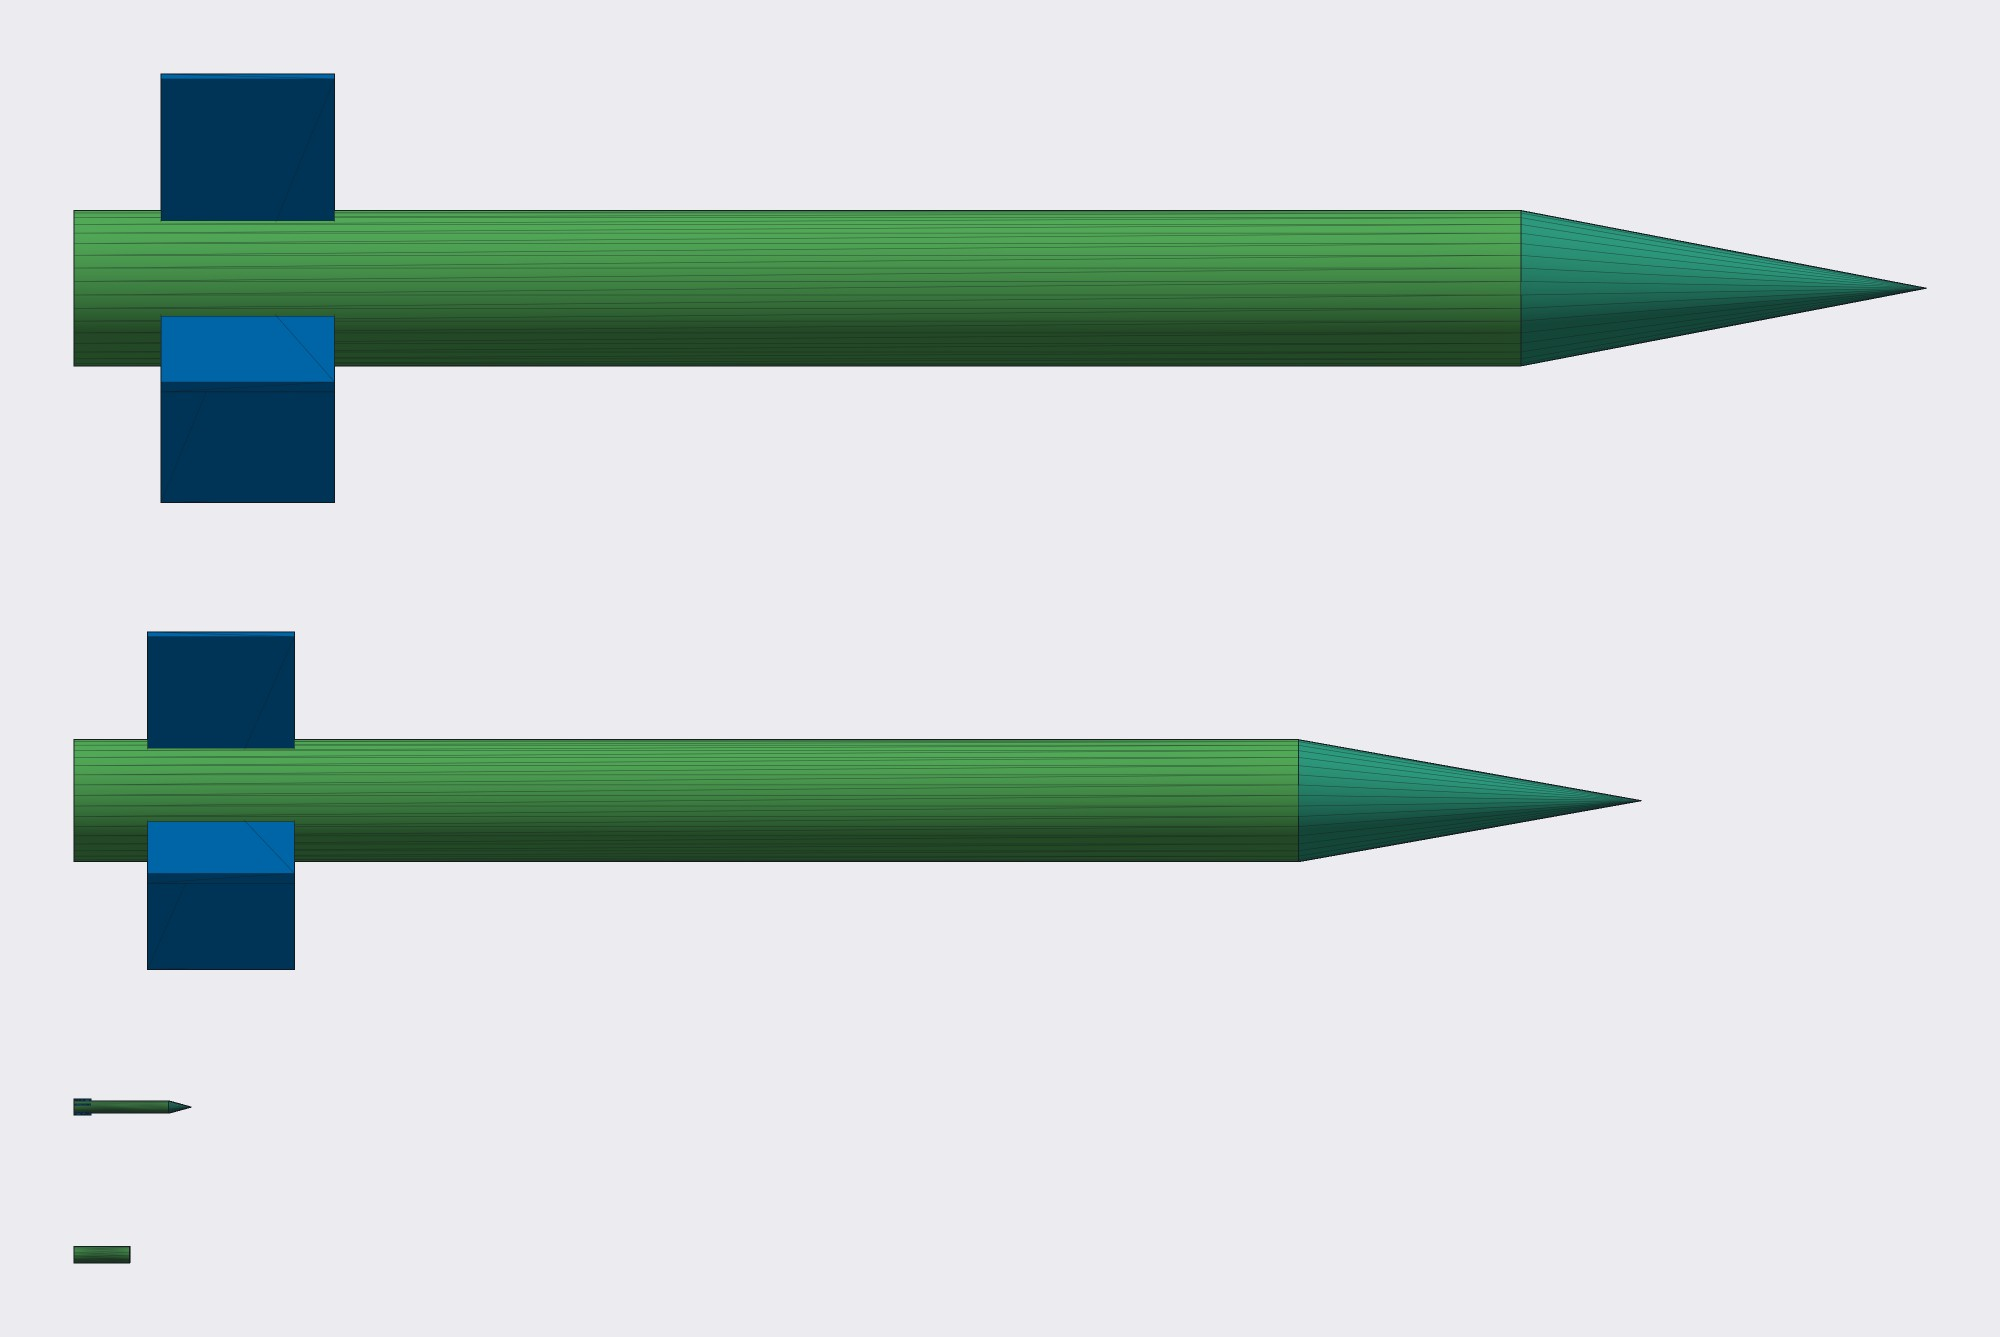
\includegraphics[width=13.00cm]{figures/img/shapes/lineup_sam_missile_mlrs_rocket_uav_round_aa_shell_casing_prims.jpg}};
\node[anchor=south west,inner sep=1pt,fill=white,fill opacity=0.8,text opacity=1] at (0.48,8.31) {SAM missile, 3.33\,m};
\node[anchor=south west,inner sep=1pt,fill=white,fill opacity=0.8,text opacity=1] at (0.48,4.69) {MLRS rocket, 2.82\,m};
\node[anchor=south west,inner sep=1pt,fill=white,fill opacity=0.8,text opacity=1] at (0.48,1.65) {UAV round, 0.21\,m};
\node[anchor=south west,inner sep=1pt,fill=white,fill opacity=0.8,text opacity=1] at (0.48,0.70) {AA shell casing, 0.10\,m};
\draw[line width=1.2pt] (12.24,0.25) -- (12.60,0.25) node[midway,above=-1pt] {10\,cm};
\end{tikzpicture}\caption{All four at one scale.}\end{subfigure}\\[1mm]\begin{subfigure}{0.62\linewidth}\centering \begin{tikzpicture}[font=\fontsize{7}{8}\selectfont]
\node[inner sep=0,anchor=south west] at (0,0) {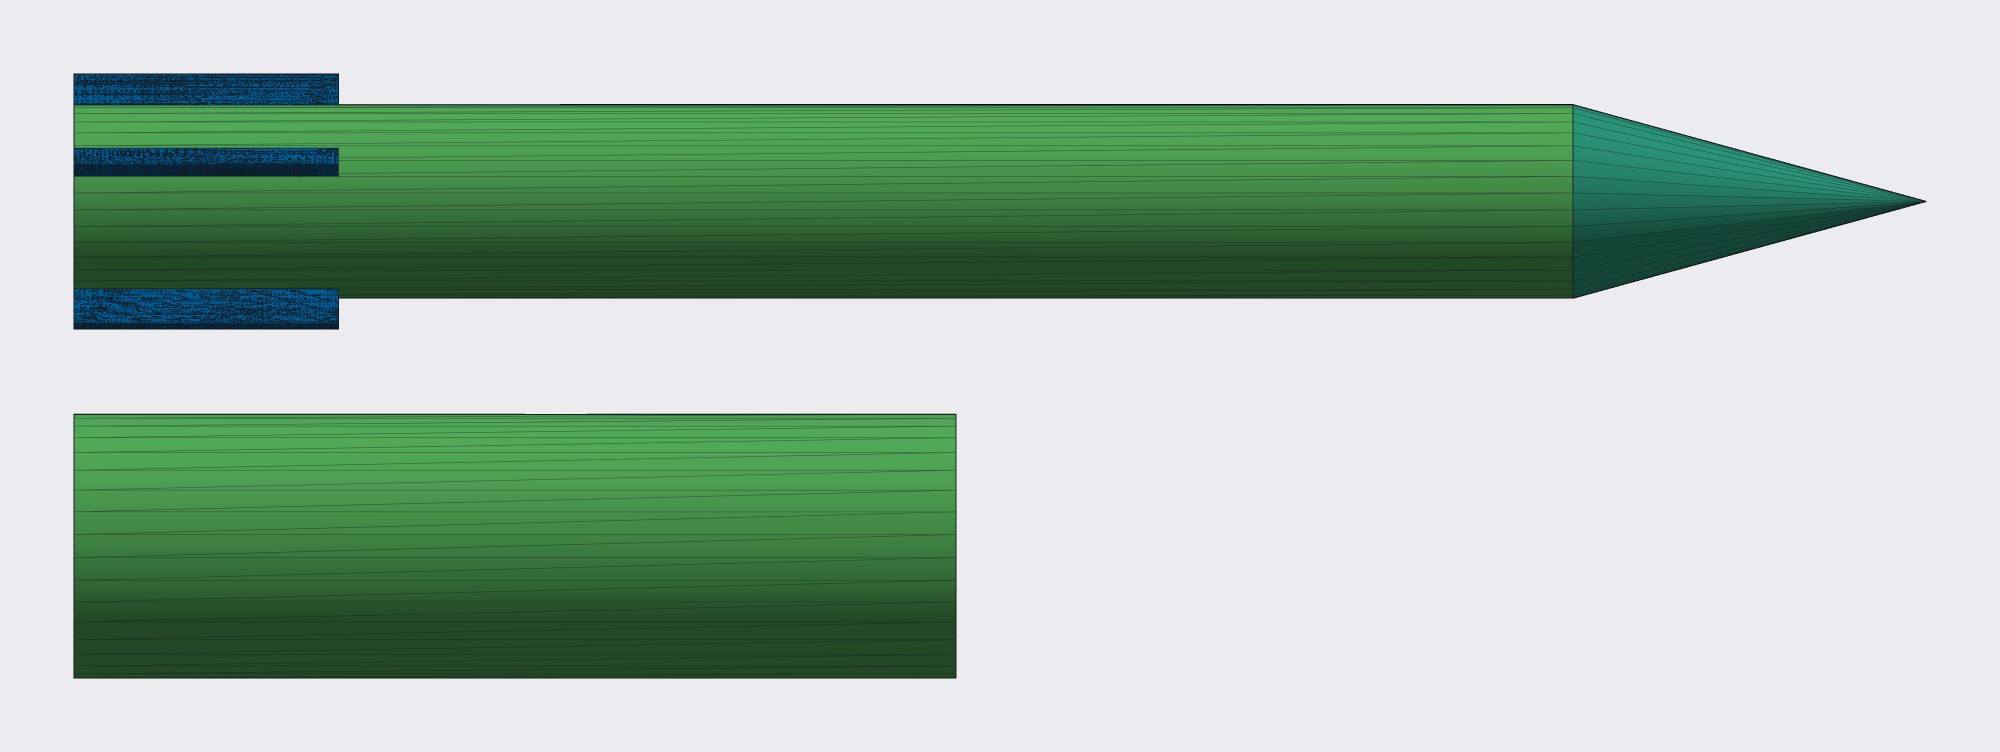
\includegraphics[width=9.00cm]{figures/img/shapes/lineup_uav_round_aa_shell_casing_prims.jpg}};
\node[anchor=south west,inner sep=1pt,fill=white,fill opacity=0.8,text opacity=1] at (0.33,3.00) {UAV round, 0.21\,m};
\node[anchor=south west,inner sep=1pt,fill=white,fill opacity=0.8,text opacity=1] at (0.33,1.59) {AA shell casing, 0.10\,m};
\draw[line width=1.2pt] (4.63,0.25) -- (8.60,0.25) node[midway,above=-1pt] {10\,cm};
\end{tikzpicture}\caption{The two small rounds enlarged (their own 10\,cm bar).}\end{subfigure}\caption{The munitions built from parts, side by side at one scale, made of primitives (orthographic, lengths along the axis are true; the exhaust flame of the missiles is left out).}\label{fig:munitions}\end{figure}}
\newcommand{\buildstripKeyUav}{\begin{subfigure}{0.245\linewidth}\img{figures/img/shapes/autonomous_uav_stage12.jpg}{\linewidth}\caption{12\,\%: 10 of 79 parts}\end{subfigure}\hfill
\begin{subfigure}{0.245\linewidth}\img{figures/img/shapes/autonomous_uav_stage35.jpg}{\linewidth}\caption{35\,\%: 28 of 79 parts}\end{subfigure}\hfill
\begin{subfigure}{0.245\linewidth}\img{figures/img/shapes/autonomous_uav_stage65.jpg}{\linewidth}\caption{65\,\%: 52 of 79 parts}\end{subfigure}\hfill
\begin{subfigure}{0.245\linewidth}\img{figures/img/shapes/autonomous_uav_stage100.jpg}{\linewidth}\caption{100\,\%: 79 of 79 parts}\end{subfigure}}
\newcommand{\buildstripKeyTank}{\begin{subfigure}{0.245\linewidth}\img{figures/img/shapes/main_battle_tank_stage12.jpg}{\linewidth}\caption{12\,\%: 31 of 255 parts}\end{subfigure}\hfill
\begin{subfigure}{0.245\linewidth}\img{figures/img/shapes/main_battle_tank_stage35.jpg}{\linewidth}\caption{35\,\%: 90 of 255 parts}\end{subfigure}\hfill
\begin{subfigure}{0.245\linewidth}\img{figures/img/shapes/main_battle_tank_stage65.jpg}{\linewidth}\caption{65\,\%: 166 of 255 parts}\end{subfigure}\hfill
\begin{subfigure}{0.245\linewidth}\img{figures/img/shapes/main_battle_tank_stage100.jpg}{\linewidth}\caption{100\,\%: 255 of 255 parts}\end{subfigure}}
\newcommand{\buildstripKeyHeli}{\begin{subfigure}{0.245\linewidth}\img{figures/img/shapes/scout_helicopter_stage12.jpg}{\linewidth}\caption{12\,\%: 11 of 91 parts}\end{subfigure}\hfill
\begin{subfigure}{0.245\linewidth}\img{figures/img/shapes/scout_helicopter_stage35.jpg}{\linewidth}\caption{35\,\%: 32 of 91 parts}\end{subfigure}\hfill
\begin{subfigure}{0.245\linewidth}\img{figures/img/shapes/scout_helicopter_stage65.jpg}{\linewidth}\caption{65\,\%: 60 of 91 parts}\end{subfigure}\hfill
\begin{subfigure}{0.245\linewidth}\img{figures/img/shapes/scout_helicopter_stage100.jpg}{\linewidth}\caption{100\,\%: 91 of 91 parts}\end{subfigure}}
\newcommand{\buildstripKeyBunker}{\begin{subfigure}{0.245\linewidth}\img{figures/img/shapes/command_bunker_stage12.jpg}{\linewidth}\caption{12\,\%: 52 of 427 parts}\end{subfigure}\hfill
\begin{subfigure}{0.245\linewidth}\img{figures/img/shapes/command_bunker_stage35.jpg}{\linewidth}\caption{35\,\%: 150 of 427 parts}\end{subfigure}\hfill
\begin{subfigure}{0.245\linewidth}\img{figures/img/shapes/command_bunker_stage65.jpg}{\linewidth}\caption{65\,\%: 278 of 427 parts}\end{subfigure}\hfill
\begin{subfigure}{0.245\linewidth}\img{figures/img/shapes/command_bunker_stage100.jpg}{\linewidth}\caption{100\,\%: 427 of 427 parts}\end{subfigure}}
